\documentclass{book}
\usepackage[T1]{fontenc}  % Use T1 encoded cm-super fonts.
\usepackage{lmodern}
\usepackage{microtype}    % Improve typesetting.
\usepackage[labelfont=bf]{caption}
\usepackage{graphicx, subfig}                     % Figures.
\usepackage[dvipsnames,rgb]{xcolor} % For defining colors.
\usepackage{ifthen}                               % For comparison.
\usepackage[a-2u]{pdfx}
\usepackage{bookmark}
\usepackage[a4paper, left=1.25in, right=1in, top=1in, bottom=1in, includehead]{geometry}
\usepackage{booktabs, colortbl} % Tables.
\usepackage{tabularx}           % Auto column sizing.
\usepackage{siunitx}
\usepackage{placeins}
\usepackage{xspace}
\usepackage{appendix}
\usepackage{wrapfig}
\usepackage[backend=biber, style=authoryear, sortcites=true, maxbibnames=3, maxcitenames=1, backref=true]{biblatex}
\usepackage{multirow}
\usepackage{makecell}
\usepackage{titlesec}
\usepackage{amssymb,amsmath}

\titleformat{\chapter}[display]
  {\normalfont\huge\bfseries}{}{0pt}{\Huge}

\PassOptionsToPackage{hyphens}{url}
\hypersetup{colorlinks=true, linkcolor={OliveGreen}, citecolor={blue}, urlcolor=blue}
\addbibresource{biblio.bib}
\DefineBibliographyStrings{english}{%
  backrefpage = {page},% originally "cited on page"
  backrefpages = {pages},% originally "cited on pages"
}
\AtBeginRefsection{\GenRefcontextData{sorting=ynt}}
\AtEveryCite{\localrefcontext[sorting=ynt]}
\captionsetup{font=footnotesize,labelfont=footnotesize}
\renewcommand\cellalign{lc}

\newcommand{\pref}[2]{(\autoref{#1}#2)}
\newcommand{\aref}[2]{\autoref{#1}#2}


\newcommand{\IntClearDoublePage}{\clearpage{\pagestyle{empty}}}
% -----------------------------------------------------------------------
% T O C    L O F    L O T    L O A
% 

% Using tocloft, the toc can be formatted easily.
\RequirePackage[titles, subfigure]{tocloft}

% Remove dots.
\renewcommand{\cftdotsep}{\cftnodots}

% Format chapter entries differently in toc.
\renewcommand{\cftchapfont}{\bfseries}

% Fix the indentation of figure and table entries in the lof, lot, and loa.
\setlength{\cftfigindent}{0in}
\setlength{\cfttabindent}{0in}

\newcommand{\AddToc}{\tableofcontents\IntClearDoublePage}
\newcommand{\AddLof}{%
	\newpage
	\phantomsection % Requires hyperref; this is to fix the link.
	\addcontentsline{toc}{section}{\numberline{}\hspace{-.35in}{\bfseries{}List of Figures}}
	\listoffigures
	\IntClearDoublePage
}
\newcommand{\AddLot}{%
	\newpage
	\phantomsection % Requires hyperref; this is to fix the link.
	\addcontentsline{toc}{section}{\numberline{}\hspace{-.35in}{\bfseries{}List of Tables}}
	\listoftables
	\IntClearDoublePage
}

% -----------------------------------------------------------------------
% F R O N T M A T T E R
% 
% The frontmatter environment set the page numbering to lowercase roman for 
% ack, abstract, toc, lof, lot, loa, etc. It also resets page numbering for the 
% remainder of thesis (arabic, starting at 1).
\renewenvironment{frontmatter}
{%
 	\setcounter{page}{1}
	\renewcommand{\thepage}{\roman{page}}
}
{%
	\clearpage
	\renewcommand{\thepage}{\arabic{page}}
	\setcounter{page}{1}
}
\usepackage[backend=biber, style=authoryear, maxbibnames=3, maxcitenames=1, backref=true]{biblatex}

\PassOptionsToPackage{hyphens}{url}
\hypersetup{colorlinks=true, linkcolor={green}, citecolor={blue}, urlcolor=blue}
\addbibresource{biblio.bib}
\DefineBibliographyStrings{english}{%
  backrefpage = {page},% originally "cited on page"
  backrefpages = {pages},% originally "cited on pages"
}

% The document.
\begin{document}
	\begin{frontmatter}
	\thispagestyle{empty}
\begin{center}
    \LARGE{CHARLES UNIVERSITY} \\
    \vspace{0.2in}
    \large{Faculty of Science} \\
    \vspace{0.2in}
    \large{Department of Physical and Macromolecular Chemistry} \\
    \vspace{0.4in}
    \begin{figure}[h!tb]
        \centering
        
\includegraphics[scale=0.6]{Figures/CharlesU.png}
    \end{figure}
    \vspace{0.4in}
    \uppercase{\LARGE{\bf{Interaction dynamics of cytoskeletal polymers}}} \\
    \vspace{0.2in}
    \uppercase{\Large{Studium dynamiky cytoskeletálních POLYMERÚ}} \\
    \vspace{0.4in}

    \large{M.Sc. Jochen Krattenmacher} \\
    \vspace{0.1in}
    \large{Doctoral thesis} \\
    \vspace{0.1in}
    \large{Supervisor: RNDr. Zdeněk Lánský, PhD.} \\
    \vspace{0.1in}
    \large{Prague 2024}
\end{center}
	\chapter*{Declaration}
I declare that I wrote this thesis independently and cited all the information sources and literature used. I also declare that I indicated the contributions of co-authors appropriately. In particular, certain parts of data acquisition of the tau-related experiments were performed by Valerie Siahaan (a member of the Laboratory of Structural Proteins), as described in the "Publications" section of this thesis. No substantial part of this work has been submitted for the award of any other or the same academic degree, though a small share of the results presented in this thesis was also presented in the doctoral thesis by Valerie Siahaan, which was difficult to avoid given our tight collaboration during some of the time of my work in the Laboratory of Structural Proteins and us consequently sharing first-authorship in our publication "Kinetically distinct phases of tau on microtubules regulate kinesin motors and severing enzymes." The figure panels which have also been presented in Valerie's thesis (\cite{Siahaan}) are marked as such in the respective figure captions.\\

\begin{minipage}{5in}
    \vspace{0.5in}
    In Berlin, 4th of October 2024 \hfill Jochen Krattenmacher
\end{minipage}
	\chapter*{Acknowledgements}
Zdenek
Marcus
Valerie
Manuel and Francois
Ilia
Janci
Lenka
Whole lab
Imaging facility
Other coauthors
%
	% 	% \begin{abstract}
However, the underlying molecular mechanism of how tau as an intrinsically disordered protein can fulfill such regulative functions is still unknown. Here we study how the collective behaviour of tau can influence the activity of motors and severing proteins on microtubules. Using in vitro reconstitution assays, we found that on the microtubule surface tau can form cohesive islands in a pool of diffusible tau molecules. We observed that the islands prevented the interaction of katanin and kinesin-1 motors with the microtubule surface. In contrast, super-processive kinesin-8 motors, which, like katanin and kinesin-1 were able to bind to and move in the regions on the microtubule surface occupied by diffusible tau molecules, additionally, could penetrate the islands where they caused island disassembly. Our results show that two kinetically distinct phases of tau, consisting, respectively, of cooperatively and discretely binding molecules, co-exist on microtubules and differentially regulate the interactions of MAPs with the microtubule surface.
\end{abstract}
	\AddToc%  Table of contents.
	% \AddLof%  List of figures.
	% \AddLot%  List of tables.
	\end{frontmatter}
   
	\chapter{Background}
The biologist Carl Woese suggested that “Organisms are resilient patterns in a turbulent flow—patterns in an energy flow” \parencite{Woese}. If this somewhat captures life, then the formation and maintenance of patterns are essential. On the sub-cellular level, an important component conferring structure and organization is the cytoskeleton. The cytoskeleton is a complex, dynamic network of protein filaments which can be found in the cytoplasm of all cells, including bacteria and archaea. Eukaryotes employ three different types of filaments: microtubules, actin filaments and intermediate filaments. These filaments interact interact with a plethora of other biopolymers in the cell, allowing the cytoskeleton to fulfill vital functions in a diverse set of domains, such as locomotion of the cell, maintaining structural integrity, chromosome segregation and cytokinesis during mitosis and the transport of cargoes within the cell. The cytoskeleton confers structure to the cell, but what confers structure to the cytoskeleton itself? While some of the patterning stems from interactions with other large entities, such as the cell membrane, the organization of the cytoskeleton partly emerges from the collective behavior of the involved cytoskeletal polymers. In other words, the cytoskeleton and its associates are known to display self-organization \parencite{Karsenti2008}. This work aims to expand our understanding of how, and to which extent, cytoskeletal polymers interact to give rise to supramolecular patterning. \par
To minimize the number of factors which could possibly give rise to patterns such to reveal underlying molecular mechanisms, we followed a bottom-up approach, where we sought to reconstitute cytoskeletal features \textit{in-vitro} with a minimum number of components. We focused on microtubules, where we were interested in two cytoskeletal systems of which they are prominent members: (1) Axonal microtubule arrays and (2) the mitotic spindle. These two systems are very different, which is reflected in the different behavior of microtubules within them. Thus, this thesis contains two parts, each dedicated to one of these systems. Each of them is introduced below, together with the microtubule-associated proteins explored in the respective experiments (see \autoref{sec:neuron} for axonal microtubule arrays and \autoref{sec:spindle} for the mitotic spindle). As in both systems, microtubules are an integral part of the experimental setup, I in \autoref{sec:microtubules} offer an introduction to them. I also give a brief primer on the biological, chemical and physical characteristics of proteins in general (\autoref{sec:proteins}), as well as on the most prominent methods used in the course of this work \pref{sec:methods_intro}{}.

\section{Foundations}
\subsection{Proteins}
\label{sec:proteins}
TODO: mention intrinsically disordered proteins

\subsection{Microtubules}
\label{sec:microtubules}
Microbules are long hollow tubes present in all eukariotic cells. They play important roles in a number of processes, including in cell division, intracellular transport, and cell motility \parencite{Akhmanova2022}.

\subsubsection{Subunits}
\label{sec:tubulin}
Microtubules are comprised of heterodimers of the protein \textit{tubulin}. In cells, tubulin exists almost exclusively as the $\alpha\beta$-tubulin heterodimer. $\alpha$- and $\beta$-tubulin are conserved throughout eukaryotes, sharing over 40\% sequence identity with nearly the same secondary and tertiary structures \parencite{DOWNING199816}. Each tubulin monomer is a globular protein and consists of three closely interacting domains: an N-terminal nucleotide-binding domain, an intermediate domain, and a carboxy-terminal (C-terminal) helical region \parencite{ALUSHIN20141117}. The disordered, negatively charged C-terminal tails of tubulin protrude outwards from the microtubule surface.\par

As is the case with many other proteins, tubulins express in different isoforms, arising from the expression of alternative tubulin-encoding genes. In humans, $\alpha$- and $\beta$-tubulin are encoded in 9 genes each \pcite{Janke2020}. Many, but not all, of these subtypes are highly conserved across species \pcite{Janke2020}, in other words, they are almost identical. Tubulins further can be modulated by post-translational modifications, thus providing an additional level of microtubule regulation \parencite{Janke2014}. Modification of the C-terminal region in particular has been found to affect microtubule properties and their interactions with other proteins \parencite{Janke2020}. 

\begin{figure}[h!tb]
	\centering
	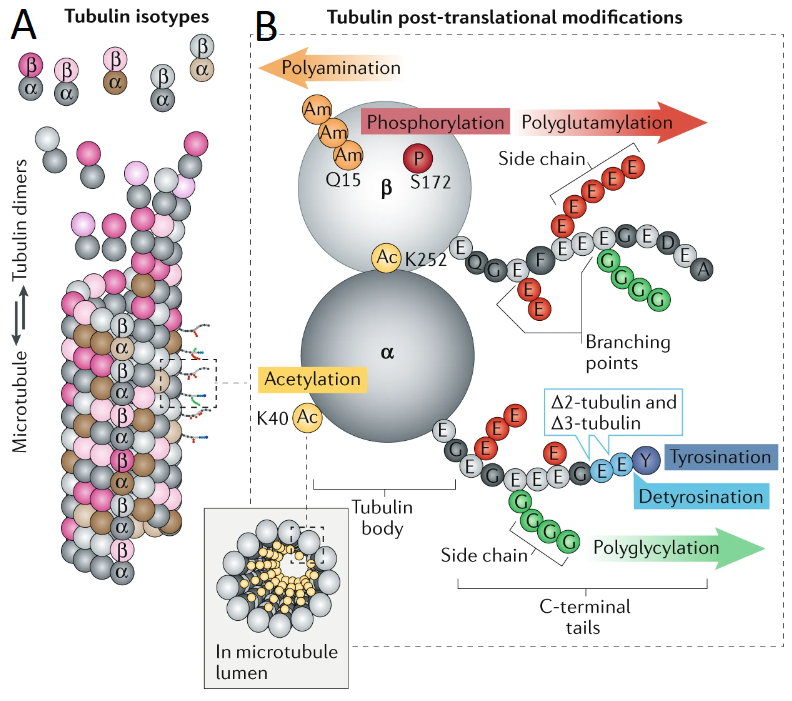
\includegraphics[width=0.6\linewidth]{Figures/tubcode.png}
	\caption[Introduction to tubulin.]{\textbf{Introduction to tubulin.}
	(A) Microtubules are constituted by $\alpha$- and $\beta$-tubulin, which in humans are expressed in different isoforms. (B) $\alpha$- and $\beta$-tubulin can undergo various types of post-translational modifications. This includes additions of groups, mainly to the C-terminal of either tubulin, but also other sites, e.g., the acetylation of a $\alpha$-tubulin residue pointing toward the inside of the microtubule (the lumen). It also includes detyrosination, which is the removal of a tyrosine from the $\alpha$-tubulin C-terminal. Taken from \cite{Janke2020}.
		}\label{tubcode}
\end{figure}

\subsubsection{Structure}
The microtubule lattice can be described as a lateral association of so-called protofilaments, which are linear strands of $\alpha$- and $\beta$-tubulin heterodimers (\autoref{MTintro}A). Their arrangement in a ring leads to the cylindrical structure of microtubules with an outer diameter of approximately 25 nm and an inner diameter of 17 nm (\autoref{MTintro}B, \pcite{Hawkins2010}). The hollow tube architecture of microtubules allows for the high persistence length of microtubules, which is in the low millimeter range \parencite{Hawkins2010}. This high persistence length allows MTs to stretch over distances comparable to the size of a whole cell. Owing to the uniform orientation of the tubulin dimers, microtubules are directional polymers, with the $\beta$-subunits pointing to one end (called ‘plus end’) and the $\alpha$-subunits pointing to the opposite end (called ‘minus end’). \par

In cells, microtubules usually have 13 protofilaments, however, in some cell types, microtubules with a different number of protofilaments have been observed, with observed numbers ranging from 11 to 15. For example, the nerve cords of nematodes harbour MTs with 11 protofilaments, and 15-protofilament microtubules have been found in various animal cells implicated in mechanosensation \parencite{Chaaban2017}. Meanwhile, microtubules polymerized \textit{in vitro} feature between 9 and 16 protofilaments \parencite{Chaaban2017}. The number of protofilaments appears to be partially determined by the isotype of the involved tubulin dimers \parencite{Ti2018}. \textit{In vitro}, the number of protofilaments also depends on whether and how the microtubules have been stabilized \aref{sec:stabilization}{}. This flexibility in terms of protofilament number allows for lattice defects to occur where the number of protofilaments may differ in different parts of a given microtubule \pcite{Chretien}. It is also worth noting that depending on the number of protofilaments, the protofilaments in a given microtubule align differently: In the 13-protofilament variant, microtubules have a helical pitch of 1.5 dimers, i.e., their structure repeats every 1.5 dimers. Here, protofilaments are in an arrangement where tubulin subunits laterally associate with the opposite type (i.e., $\alpha$- with $\beta$-tubulin), except at the seam, where tubulins of the same type associate (\autoref{MTintro}B). A different number of protofilaments typically results in a different pitch, and in some instances in microtubules without a seam \pcite{Hawkins2010}. Finally, a different number of protofilaments typically results in a structure where protofilaments no longer are straight but curl around the microtubule \parencite{Chaaban2017}.

\subsubsection{Polymerization}
\label{sec:instability}
Microtubules grow in every eukaryotic cell and can also be polymerized \textit{in vitro}, i.e., in assays outside of cells given an adequate experimental buffer. Notably, the spontaneous assembly of microtubules, i.e., spontaneous \textit{microtubule nucleation}, is kinetically unfavorable because the intermediate tubulin structures required for forming a full ring are not very stable \parencite{Akhmanova2022}. Spontaneous nucleation thus can occur only at high concentrations of free tubulin \parencite{Fygenson1994}. In a more kinetically favorable mechanism, the \textit{de novo} assembly of microtubules is partly directed by designated $\gamma$-tubulin nucleation complexes, which provide templates for the outgrowth of new microtubules \parencite{Akhmanova2022}. These nucleation complexes can be found in microtubule-organizing centers such as the centrosome of the spindle (\autoref{sec:spindle}), and in some cases also along pre-existing microtubules \parencite{Akhmanova2022, Janson2007}. Another means by which the cell can multiply the number of microtubules is by severing existing microtubules (\cite{Vemu2018}, see \autoref{sec:katanin_intro}). Notably, the fact that spontaneous nucleation is kinetically unfavorable gives the cell a high degree of control over the number and distribution of microtubules over time and space. \par

In spite of their high persistence length, microtubules are no static structures. Instead, their plus ends are stochastically switching between phases of growth and shrinkage \parencite{Janosi2002}. This property is termed \textit{dynamic instability}. According to the widely accepted and GTP cap model of microtubule instability \pcite{Gudimchuk2021}, microtubule dynamic instability stems from the existence of two conformationally distinct populations of tubulin dimers: GTP-tubulin and GDP-tubulin, having GTP respectively GDP bound to their $\beta$-tubulin. Mostly, it is free GTP-tubulin that adds to the lattice of a polymerizing microtubule. Shortly after polymerization, the $\beta$-tubulin hydrolyzes its GTP, resulting in conformational changes which result in mechanical tension. GTP-hydrolysis of a lattice-incorporated tubulin has no immediate consequences for the microtubule as a whole. However, if GTP-hydrolysis occurs at a microtubule end, the higher degree of freedom allows for conformational relaxation and eventual removal of GDP-tubulin from the microtubule end. This conformational relaxation typically takes the form of a curving of the protofilament, breaking lateral bonds with neighbouring protofilaments and thereby further destabilizing the microtubule end. Thus, if a microtubule loses too many GTP-tubulins at its plus end, i.e., if it loses its GTP cap, it switches to a regime of quick depolymerization where most protofilaments are curved outwards (\autoref{MTintro}C). While the GTP cap model of dynamic instability is experimentally strongly supported, there is less clarity on why exactly GTP-tubulin lattices are more stable than GDP-lattices, and multiple, non-mutually-exclusive models exist \pcite{Gudimchuk2021}. In one model, GTP tubulin dimers are straighter than GDP tubulin dimers already in their relaxed state, facilitating their lattice incorporation. In another model, GTP tubulin might more readily change into a straight conformation than GDP tubulin. A third model proposes that GTP hydrolisis introduces relevant conformational changes at the interface between the adjacent dimers of a given protofilament. There certainly is evidence that GTP hydrolisis introduces changes at these interfaces \pcite{Alushin2014}.\par

A change from continued polymerization to rapid depolymerization is called a \textit{catastrophe} event. A reversal from depolymerization to polymerization can also occur and is called a \textit{rescue} event. In the absence of rescue-promoting microtubule-associated proteins \pref{sec:MAPs}{}, rescues are currently hypothesized to occur mainly at positions where GTP islands have formed within the otherwise GDP-dominated microtubule lattice. This hypotehsis is supported by \textit{in vitro} experiments showing rescues to coincide with GTP islands \pcite{Aumeier2016}. These islands had further been shown to be the result of microtubule self-repair, i.e., instances where free GTP-tubulin was incorporated into a damaged part of the microtubule \pcite{Aumeier2016}. Recently, microtubule self-repair and GTP islands have also been observed \textit{in vivo} \pcite{Gazzola2023}.\par

As a final note, microtubule minus ends \textit{in vivo} have not been observed to elongate, i.e., microtubule polymerization happens exclusively at the plus end \parencite{dammer}. \textit{In vitro}, minus ends can also exhibit polymerization, yet the plus end nonetheless polymerizes more quickly and is generally more dynamic \parencite{Howard2003}. 

\begin{figure}[h!tb]
\centering
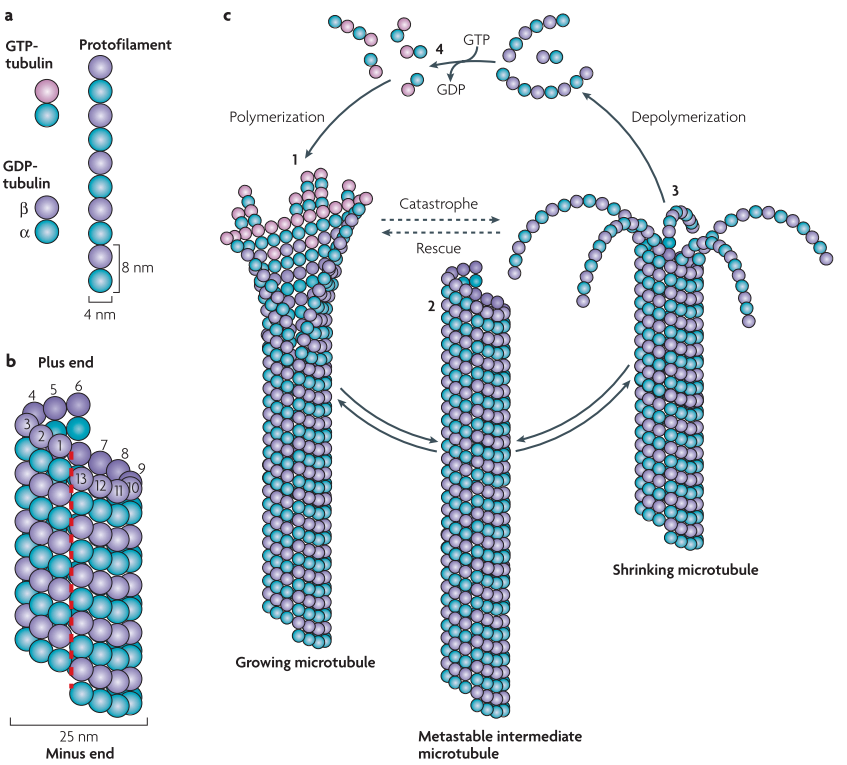
\includegraphics[width=\linewidth]{Figures/MTintro.png}
\caption[Introduction to microtubules.]{\textbf{Introduction to microtubules.}
(A) Microtubules consist of $\alpha\beta$ heterodimers. While $\alpha$-tubulin normally retains its GTP, the GTP molecule of $\beta$-tubulin can be both hydrolyzed and exchanged for ADP. (B) \textit{In vivo}, microtubules are composed of 13 protofilaments. Since the \SI{12}{\nm} helical pitch does not equal the dimer length, a lattice seam occurs. (C) Due to the GTP-hydrolysis of incorporated $\beta$-tubulin, microtubule ends undergo a permanent cycle of growth (1) and shrinkage (3), closed by the exchange of GDP for GTP for the disassembly products (4). This cycle can briefly come to a halt during a less prevalent metastable state (2), from which microtubules can switch either to growth or to shrinkage. All sketches adapted from \cite{Akhmanova2008}.
	}\label{MTintro}
\end{figure}

\FloatBarrier

\subsubsection{Microtubule-associated proteins}
\label{sec:MAPs}
The vast functional diversity of microtubules is enabled by their interactions with microtubule-associated proteins (MAPs). \cite{BODAKUNTLA2019804} categorize MAPs into different groups depending on their mode of action, namely i) molecular motors generating movement along microtubules, ii) enzymes destabilizing the microtubule lattice, iii) MAPs promoting microtubule nucleation, iv) microtubule-end binding proteins and v) structural MAPs controlling microtubule polymerization, stabilization and assembly into microtubule bundles. One MAP may belong to several of these groups, for instance, the molecular motor Kip3 is known to also cause microtubule polymerization \parencite{Gardner2011a}. In the course of my work, I have worked with four different MAPs as introduced further below, namely tau \pref{sec:tau_intro}{}, kip3 \pref{sec:kip3_intro}{}, katanin \pref{sec:katanin_intro}{}, and Ase1 \pref{sec:Ase1_intro}{}. 

\subsection{Employed technologies}
\label{sec:methods_intro}
Below a primer on some of the main technologies which enabled the work performed for this thesis.

\subsubsection{In-vitro stabilization of microtubules}
\label{sec:stabilization}
For in-vitro experiments, it often is desirable to stabilize microtubules such that they remain polymerized even in the absence of GTP and/or free tubulin, in other words, to prevent microtubule instability. There are two popular methods, which I had both employed during my work:
\begin{itemize}
	\item \textbf{Stabilization via GMPCPP.} GMPCPP is a non-hydrolyzable analog of GTP that binds to the GTP-binding site of tubulin. By mimicking GTP, GMPCPP stabilizes the microtubule lattice, without any hydrolisis occurring which would normally induce lattice instability. This stabilization allows microtubules to remain polymerized even in the absence of free tubulin, GTP, or GMPCPP \parencite{Hyman1992}.
	\item \textbf{Stabilization via paclitaxel}. Paclitaxel, also known as taxol, does not directly interfere with the GTP cycle of tubulin but rather binds along the microtubule. This binding enhances microtubule stability, even under conditions that would normally induce shrinkage, such as low tubulin concentrations \parencite{SCHIFF1979}. Notably, paclitaxel is not tightly bound to microtubules \pcite{Diaz98}, and thus paclitaxel-stabilized microtubules need to be stored in buffer solutions containing paclitaxel.
\end{itemize}
It is worth noting that the choice of stabilization impacts the mechanical properties of microtubules. For example, paclitaxel-stabilized microtubules tend to have fewer protofilaments than GMPCPP-stabilized microtubules. Paclitaxel-stabilized microtubules feature a wide variability in their protofilament number, with the most common number being 12 protofilaments, while GMPCPP-stabilized microtubules typically feature 14 protofilaments \pcite{Andreu1992, Meurer}. Also, GMPCPP-stabilized microtubules have been measured to have twice the flexural rigidity of paclitaxel-stabilized microtubules \pcite{Mickey1995}.

\subsubsection{Labelling with fluorescent proteins}
The first discovered fluorescent protein is green fluorescent protein (GFP), which was discovered around 60 years ago in the jellyfish Aequorea victoria \pcite{shimomura2005discovery}. Today, due to the discovery of new fluorescent proteins in other species as well as genetic engineering, a range of fluorescent proteins with different characteristics are available for use in laboratory work \pcite{Kremers2011}. A common use case of fluorescent proteins, as made use of in this work, is labeling a protein of interest, thereby allowing for determining the location of the protein of interest via fluorescence microscopy techniques (see below). To achieve this labeling, the gene encoding the protein of interest is joined with the gene encoding a given fluorescent protein via recombinant DNA technology. Expressing this DNA construct then yields the protein of interest fused to the fluorescent protein. Notably, despite the relatively large size of fluorescent proteins (they all have a size around 27 kDa, compare e.g. to Ase1 with a size of 83 kDa), fusing them either to the C- or the N-terminal of a given protein usually does not significantly impair its function \pcite{Kremers2011}. 

\subsubsection{Total internal reflection (TIRF) microscopy}
The main experimental method employed during the course of this work was total internal reflection fluorescence (TIRF) microscopy. TIRF microscopy takes advantage of the physical phenomenon of total internal reflection, whereas light is fully reflected from a surface, yet a so-called evanescent field emanates beyond the surface of reflection, decaying exponentially in intensity. Because the evanescent field does not propagate, this phenomenon allows to selectively illuminate fluorophores near the glass/water surface, in our case the immobilized microtubules and their associated MAPs. By avoiding to excite fluorophores further away from the immobilized microtubules, background fluorescence can be reduced, as mainly the fluorophores of interest are excited. This is crucial for assays with a large number of labeled proteins in solution. 

The main experimental method employed during the course of this work was total internal reflection fluorescence (TIRF) microscopy. TIRF microscopy is a specialized technique derived from fluorescence microscopy, which itself is a powerful tool used to study the distribution of fluorophore-labeled molecules within cells and other biological samples. Fluorescence microscopy relies on the excitation of fluorophores by specific wavelengths of light, leading to the emission of light at a longer wavelength. This process enables the visualization of structures and molecules with high specificity due to the different spectral signatures of different dyes or proteins \pcite{Lichtman2005}. A higher specificity can be achieved by employing optical filters, which for instance is useful when working with multiple fluorophores in the same sample. Optical filters can be employed to minimize "bleeding" of the signal of one fluorophore when aiming to detect the signal of the other.\par

TIRF microscopy, in particular, takes advantage of the physical phenomenon of total internal reflection, where light is fully reflected at the interface between two media with different refractive indices, such as glass and water. Although the light is fully reflected, a so-called evanescent field extends beyond the surface of reflection, decaying exponentially in intensity. This non-propagating field allows for the selective excitation of fluorophores located within approximately 100 nm of the glass/water interface, making it ideal for visualizing surface-bound molecules \pcite{Mattheyses2010}. In our experiments, TIRF microscopy was used to illuminate fluorophores associated with immobilized microtubules and their associated microtubule-associated proteins (MAPs). By restricting the excitation to fluorophores near the surface, background fluorescence from molecules further away from the surface is significantly reduced, improving the signal-to-noise ratio. This selective excitation is crucial in assays involving a large number of labeled proteins in solution, as it ensures that only the fluorophores of interest contribute significantly to the observed fluorescence signal \pcite{Mattheyses2010}.

\subsubsection{Interference reflection microscopy (IRM)}
For a few experiments (as indicated in methods section) we had employed interference reflection microscopy (IRM). In contrast to fluorescence-based microscopy methods, IRM allows for label-free imaging of biological samples. In the IRM setup, light from the light source passes through the aperture diaphragm and the field diaphragm, which regulate the amount of light reaching the camera. The 50/50 mirror then divides the light into two beams: one transmitted and one reflected, each with half the intensity of the original beam. The reflected beam is directed toward the objective, reflects off the sample, and then travels back through another 50/50 mirror and the tube lens to the camera. The resulting image is determined by the interference of reflections at the glass/water and water/sample interfaces. These reflections are influenced by differences in refractive indices — greater differences result in higher intensity of the reflected light beam \parencite{barr2009interference}. IRM thus requires particles large enough to generate noticable shifts in the phase of the reflected light. Due to the relatively large size of microtubules, IRM can be used to visualize them, with the advantage of requiring relatively few changes to typical microscope setups compared to more advanced techniques such as interferometric scattering (iSCAT) microscopy \parencite{Mahamdeh2018}.

\subsubsection{Fluorescence recovery after photobleaching (FRAP)}
\label{sec:FRAP}
We for a few experiments also employed fluorescence recovery after photobleaching (FRAP) to investigate the binding kinetics of microtubule-associated proteins (MAPs). In the FRAP setup, a focused laser, in our case using the TIRF setup, is used to photobleach fluorescently-labelled molecules within a given region, creating a dark spot. The recovery of fluorescence in this region is then monitored over time as unbleached molecules diffuse into or associate with the bleached microtubule area, while bleached molecules dissociate or move away \parencite{axelrod1976mobility}. FRAP was a relevant for us due to its ability to provide insights into the unbinding rate $k_{off}$ of a given microtubule-associated protein. If the binding sites on a microtubule for a given MAP are covered such that an equilibrium exists (i.e. no net binding or unbinding of MAPs occurs), after bleaching all of the MAPs on that microtubule, the rate of recovery depends only on $k_{off}$, assuming that the fluorescent MAPs in solution were not significantly depleted by the photobleaching \parencite{bulinski2001rapid}, which in our case is true due to our employment of TIRF. Specifically, to determine $k_{off}$, one can fit the following function to the signal $I(t)$ measured experimentally by imaging the region over time (taking care to not signficantly bleach the sample due to this imaging): $I(t)=1-e^{-k_{off}t}$ \parencite{bulinski2001rapid}.

\section{Microtubule systems}
Microtubules behave differently and fulfill different functions depending on the cellular context they are in. The two systems where I with this thesis aim to contribute understanding to are axonal microtubule systems (with a focus on tau, katanin, and kinesin-8) and the mitotic spindle (with a focus on Ase1).

\subsection{Axonal microtubule arrays}
\label{sec:neuron}
The complex development and functionality of the nervous system rely heavily on microtubule-related processes, as microtubules play key roles in guiding cellular organization and intracellular transport \parencite{Kapitein2015}. Prominently, neurons develop two types of cytoplasmic protrusions: (i) Axons (also called nerve fibers) and (ii) dendrites. A typical neuron has one axon, which can reach to distant parts within the animal's body, and multiple dendrites, which are shorter, and connected to axons via synapses. While axons primarily contain long, stable microtubules, dendrites harbor shorter, more dynamic microtubules \parencite{Tas2017}. To understand their cellular context, it is instructive to introduce axonal microtubule arrays vis-a-vis dendritic microtubule arrays.\par

Regarding intracellular transport, microtubules prominently serve as highways for molecular motors, most prominently kinesins, but also dyneins which are minus-end directed motors \parencite{Kapitein2015}. Efficient directional transport is especially crucial in neurons, given that dendrites and especially axons grow to macroscopic lengths. It is thus not surprising that within axons, microtubules bundle and point toward the same direction, namely with their plus ends away from the cell body (the soma) toward the distal end of the axon \parencite{Tas2017}. Such an alignment lends itself to efficient transport of cargo between these distant parts of the cell, as a given motor cannot accidentally switch to an antiparallely aligned microtubule and travel in the opposite direction than previously. At the same time, within mammalian dendrites, there are both inward- and outwardpointing microtubules in equal parts \parencite{Tas2017}. Here, sufficiently effective transport is achieved by bundling microtubules such that a given bundle in a given dendrite predominantly comprises microtubules of the same orientation \parencite{Tas2017}. Notably, and puzzingly, despite the existence of plus-end-outward microtubules in dendrites, many plus-end directed motors, including kinesin-8, only enter the axon \parencite{Lipka2016}.\par

Regarding the guiding of cellular organization, the remodeling of microtubule arrays plays a central role in cell migration as well as the development of axons, dendrites, and synaptic connections \parencite{Kapitein2015}. For example, some molecular motors transport signaling factors or can even have non-motor signaling functions themselves, and as such the positioning of the microtubules becomes a determinant of developments within the cell \parencite{Hirokawa2010}. Microtubules and microtubule motors are also involved in generating mechanical forces that drive cellular processes. For instance, dynein motors, by sliding axonal microtubules against each other, can push microtubules into growth regions of the axon, thereby in their interplay with opposing kinesin motors co-determining the direction of axonal growth \parencite{Kahn2016}. Notably, post-translational modifications of tubulin (see \autoref{sec:tubulin}) play an essential role in fine-tuning MT dynamics and stability. Tubulin acetylation, for example, is associated with stable microtubules, which can be found e.g. in the axonal shaft but also in dendrites \parencite{Tas2017}. Dynamic (or "labile") microtubules, which undergo frequent cycles of growth and shrinkage, comprise less acetylated tubulin, and can be found in dendrites and at the tips of growing axons, where active remodeling is necessary \parencite{Baas2016, Tas2017}. In this context, it is also notable that Katanin levels in neurons are highest during developmental stages where a high dynamicity is required, and both depleting and overexpressing the p60 subunit have been shown to result in impaired neuronal development \parencite{Karabay2004}.\par

\begin{figure}[h!tb]
	\centering
	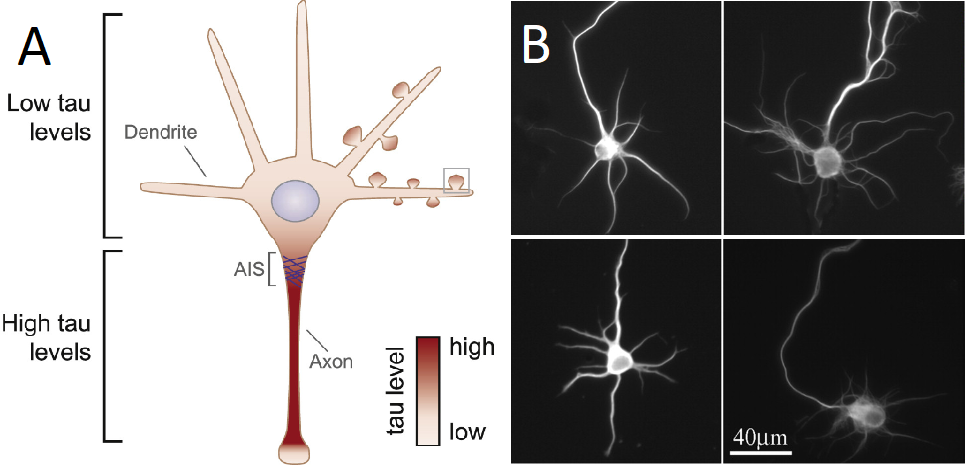
\includegraphics[width=\linewidth]{Figures/neuron.png}
	\caption[Tau in the neuronal context.]{\textbf{Tau in the neuronal context.}
	(A) Tau distribution in the neuron (adapted from \cite{Ittner2018}). Tau enrichment in the axon is facilitated by the axon initial segment (AIS) which acts as a diffusion barrier for tau. (B) Microtubule immunostains of cultured rat hippocampal neurons, adapted from \cite{Qiang2006}. Upper left: Control condition. Lower left: Depletion of tau. The panels on the right side show cells where the Katanin p60 subunit was overexpressed (with no change in tau levels in the upper panel and depletion of tau in the lower panel).
		}\label{neuron}
\end{figure}

\subsubsection{Tau}
\label{sec:tau_intro}
Tau is an intrinsically disordered protein (see \autoref{sec:proteins}) mainly found in neurons. Within the neuron, tau is mostly found in the axonal shaft, i.e. the most stable part of the neuronal microtubule architecture (\autoref{neuron}A). An important function of tau is to enhance the stability of microtubules. Tau binding for instance promotes microtubule polymerization, not only by enhancing microtubule growth rates but also by reducing the rate of catastrophes as well as depolymerization speed \parencite{Drechsel1992}. Tau binding also has been found to increase the flexural rigidity of microtubules \pcite{Mickey1995}. Tau can also stabilize microtubules via its capability to regulate the interaction of other MAPs with the microtubule surface \parencite{Morris2011b}. In particular, tau mislocalization has \textit{in vivo} been shown to protect axonal microtubules against microtubule-severing enzymes such as katanin, and its mislocalization thus leads to microtubule destabilization and the eventual degeneration of the axon (\autoref{neuron}B) \parencite{Qiang2006}. Given the importance of microtubules, and given that tau protects microtubules, it is not surprising that malfunctions related to tau have been implicated in a number of neurodegenerative diseases \parencite{Gao2018,Morris2011b,iqbal2016tau}. For example, displacement of tau from the axon is one of the hallmark events during the onset of the Alzheimer’s disease \parencite{zempel2015tau}. Conspicuously, when tau is hyperphosphorylated, i.e., contains more phosphate than normally, it aggregates into neurofibrillary tangles rather than binding to microtubules \pcite{wang2012abnormal}. \par

As depicted in \autoref{tau}A, full-length adult tau is intrinsically disordered and includes a projection domain (its N-terminal domain), a microtubule-binding region of four imperfect sequence repeats (R1-4), and a C-terminal domain \parencite{Himmler1381}. Several different observations and explanations for how tau interacts with microtubules can be found in the literature \parencite{Morris2011b,Mcvicker2014,Kellogg2018}. For instance, it is known that tau can engage with microtubules in a mode where it diffuses along the microtubule \parencite{Hinrichs2012b}, and in another mode where it is stably bound to the microtubule \parencite{Mcvicker2014}. Recently, it was found that the tau microtubule binding repeats can bind to microtubules in a consistent, orderly fashion, enough so to allow for a high-resolution cryo-EM study (\autoref{tau}B-C) \parencite{Kellogg2018}. Finally, another notable characteristic of tau is that the projection domain of tau appears to determine and cause the spacing between the microtubules within axonal microtubule arrays \parencite{Chen1992}. Previously it had been suggested that tau decoration of the microtubule might act as a "polymer brush," where the projection domains of each tau molecule cause repulsion between microtubules, thereby counteracting attraction between microtubules and causing spaces between them \pcite{Mukhopadhyay2004}. However, recent research questioned this model, arguing that the tau-tubulin ratio in cells was too low for this model, such that tau molecules could simply diffuse to other locations on the microtubule and thereby allow a given microtubule pair to align \pcite{Gaspard}. \par

Recently, it has been shown that tau protein, can undergo liquid-liquid phase separation, as had previously already been observed for some other intrinsically disordered proteins \pcite{Amayra}. Furthermore, tubulin was observed to partition into these "tau drops," and to assemble into microtubule bundles within these drops, offering another potential mechanism for microtubule nucleation in axons. 
\begin{figure}[h!tb]
\centering
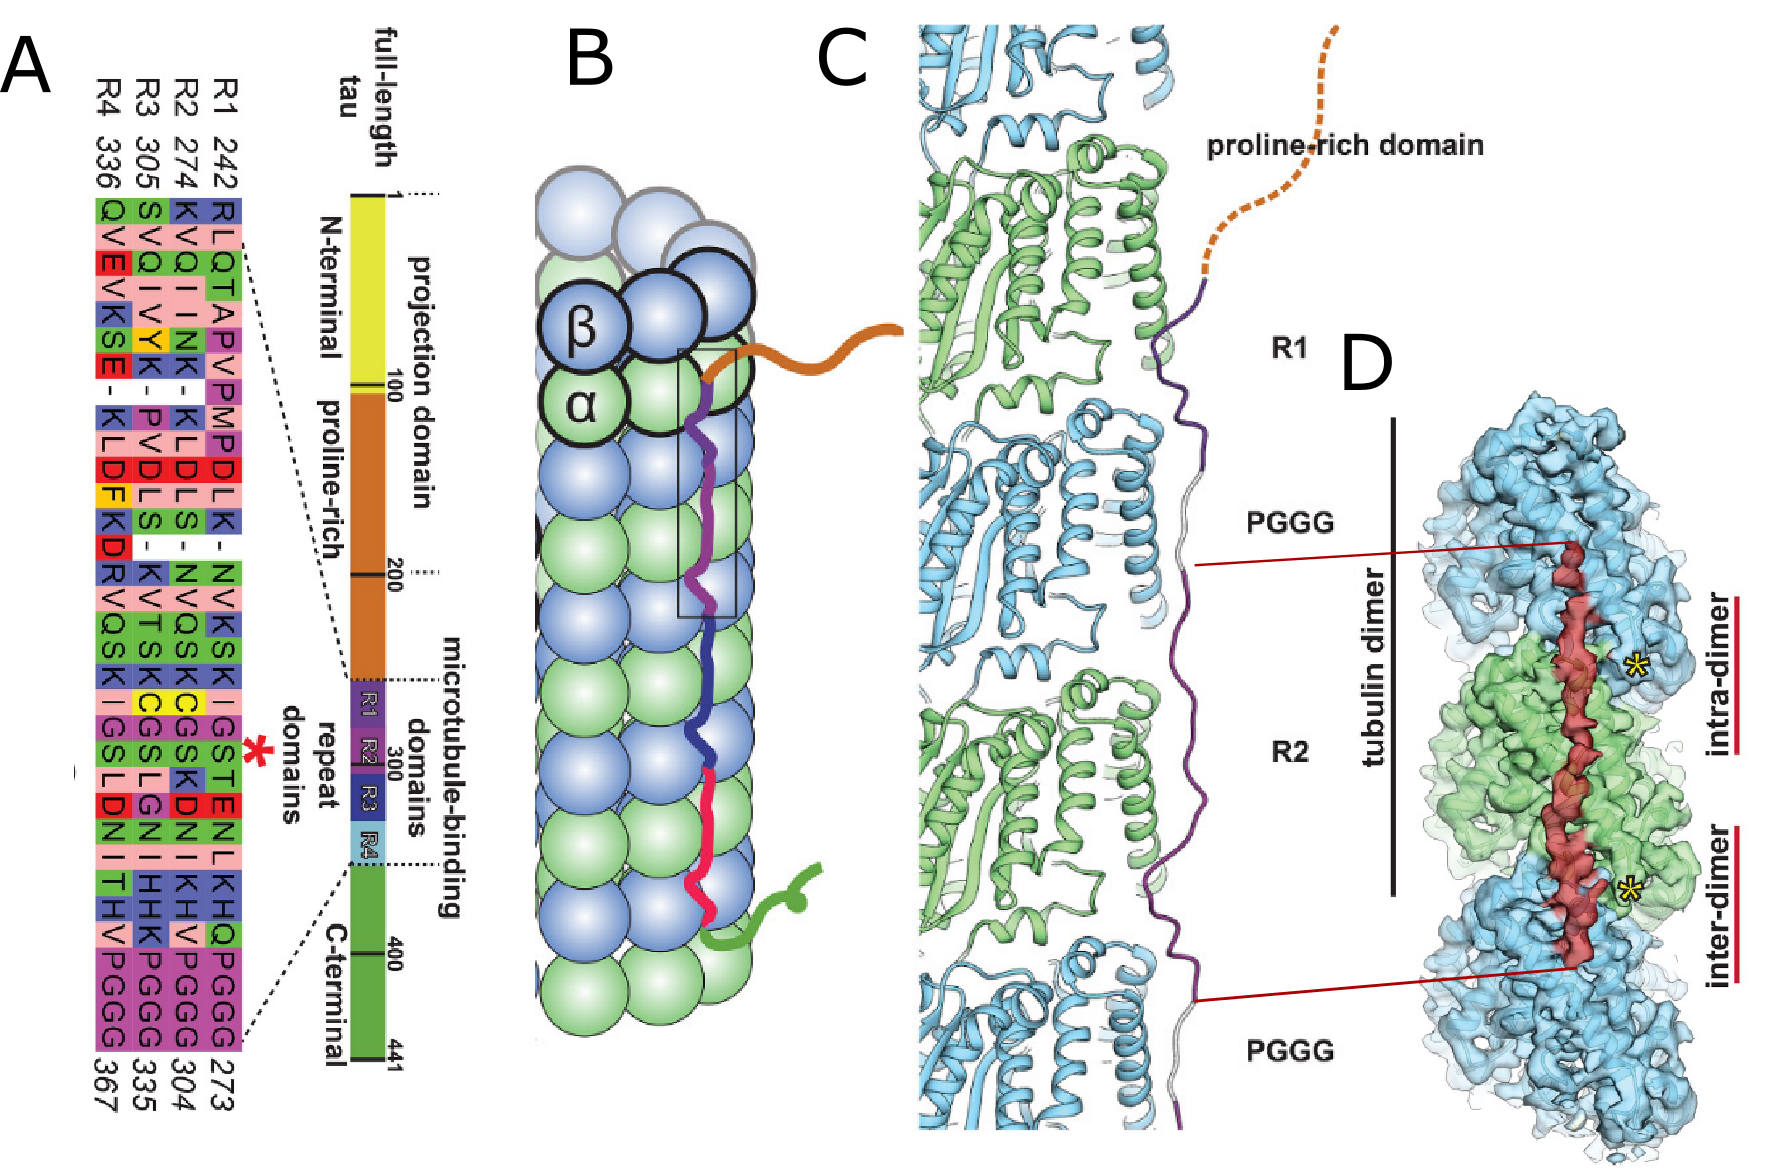
\includegraphics[width=\linewidth]{Figures/tau.png}
\caption[Introduction to tau.]{\textbf{Introduction to tau.}
(A) Schematic of the domains of tau protein. Inset shows the sequence alignment of the four microtubule binding repeat sequences, R1-4, that make up the repeat domain. (B) Model of full-length tau binding to microtubules and tubulin oligomers proposed by a recent cryo-EM study \parencite{Kellogg2018}. (C) Detailed representation of that model. (D) Cryo-EM density map of a part of the microtubule surface under the presence of tau, as observed by \cite{Kellogg2018} (top view, looking onto the surface of the microtubule). The additional density (in addition to tubulin) is colored in red and likely due to tau binding to the microtubule with its microtubule binding repeats. The PGGG sequences between the repeats were not visible on the density map, indicating that they did not bind to the microtubules in an orderly fashion. Adapted from \cite{Kellogg2018}. 
	}\label{tau}
\end{figure}

\subsubsection{Katanin}
\label{sec:katanin_intro}
Katanin is a microtubule-severing enzyme that plays a critical role in the remodeling of the microtubule cytoskeleton by generating internal breaks in microtubules. This severing function modulates microtubule dynamics and organization, contributing to essential processes such as cell division, migration, and neuronal development \parencite{ROLLMECAK201096, Lombino2019}. Katanin is a heterodimer composed of two subunits: a catalytic p60 subunit and a regulatory p80 subunit. The p60 subunit belongs to the AAA+ (ATPases Associated with various cellular Activities) protein family, containing the ATPase motor domain responsible for generating mechanical force required for microtubule severing \parencite{Johjima2015, McNally2014}. While the p60 subunit has been shown to on its own exhibit microtubule-severing activity \parencite{McNally2014}, the p80 subunit has been shown to regulate the spatial distribution of katanin by targeting katanin to the centrosome \parencite{Hartman1998}. This spatial regulation is vital, as indiscriminate severing of microtubules can lead to deleterious effects on cell function. In addition to its centrosomal localization, the p80 subunit plays a role in regulating the overall activity of the catalytic p60 subunit \parencite{McNally2000}. \par

Katanin's severing activity appears to at least partially depend on ATP hydrolysis. ATP binding and subsequent hydrolysis stimulated by the microtubule provide the energy required for conformational changes in the p60 subunit, enabling it to exert mechanical force on the microtubule lattice \parencite{Zehr2017}. Specifically, katanin is thought to pull on the C-terminal tails of tubulin subunits, destabilizing the lateral interactions between protofilaments in a step-wise manner, leading to local lattice destabilization and often microtubule breakage \pref{katanin}{}. After the microtubule breakage, whether the newly created microtubule plus end polymerizes or depolymerizes depends on the presence of free tubulin \parencite{Vemu2018, Kuo2021}. At a low free tubulin concentration, the newly-created plus end will shrink. However, if there is sufficient free tubulin present, the microtubule has a high chance of entering a growth regime, because the likelyhood is high that at the site of breakage, a sufficient number of GTP-tubulin has been incorporated, establishing a protective cap (see \autoref{sec:instability}). Similarly, it should be noted that incorporation of GTP-tublin also occurs at microtubule sites where severing is not fully completed, which can lead to the emergence of GTP islands in the lattice with higher resistance against depolymerization \parencite{Vemu2018}. These mechanisms can explain the perhaps counterintuitive phenomenon that the loss of Katanin has been found to cause a decrease in microtubule mass \parencite{Vemu2018}. 
\par
In addition to it's severing activity, Katanin also promotes depolymerization of microtubules from their ends, in a manner which is independent from ATP hydrolisis and the C-terminal tails of tubulin \parencite{Belonogov2019}.

\begin{figure}[h!tb]
\centering
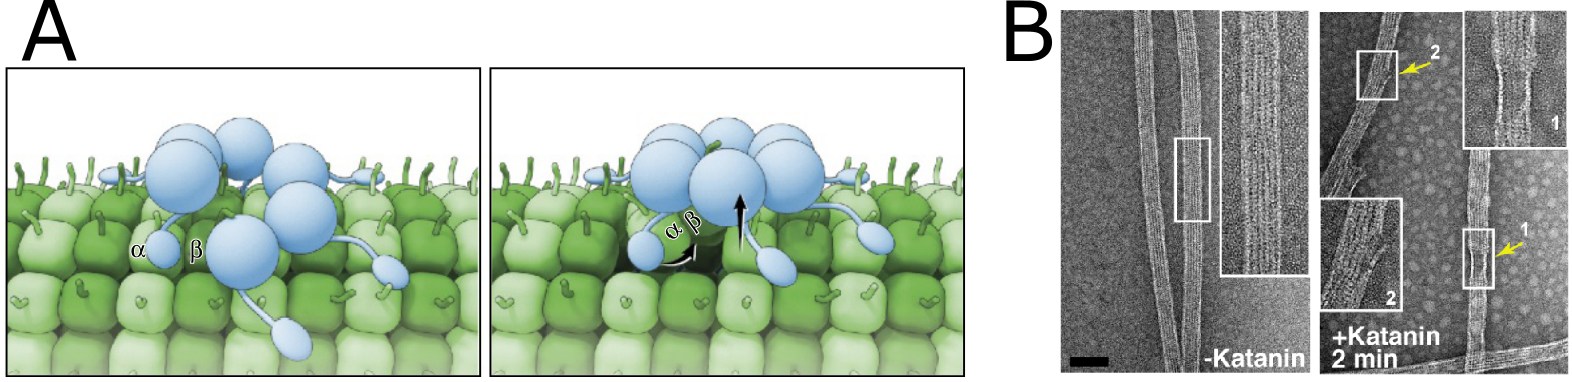
\includegraphics[width=\linewidth]{Figures/katanin.png}
\caption[Introduction to katanin.]{\textbf{Introduction to katanin.}
(A) Cartoon illustrating how the p60 subunit of katanin is hypothesized to extract tubulin dimers. Left, katanin p60 (blue) assembles as a hexamer with each monomer's N-terminal domain emanating from the motor core and making multivalent interactions with the microtubule (green). The flexible tubulin C-terminal is engaged in the axial pore of the p60 hexamer. Right, ATP hydrolysis leads to closure of the ring that drags with it the bound C-terminal tail of a tubulin monomer. The cycle is repeated until lattice contacts unravel and the microtubule severs. Adapted from \cite{Zehr2017}. (B) GMPCPP-microtubules incubated with buffer or 100 nM katanin and visualized by transmission electron microscopy. Arrows indicate damage in the microtubule lattice. Adapted from \cite{Grigorieff2018}.
	}\label{katanin}
\end{figure}

\subsubsection{Kinesin-8/Kip3}
\label{sec:kip3_intro}
Molecular motors convert chemical energy in form of ATP into mechanical energy. One of the three large superfamilies of molecular motors are kinesins. To date more than 600 kinesin sequences with 45 kinesin genes in the human- 17 -genome \parencite{Endow3420} have been identified. Kinesins are divided into 14 kinesin sub-families based on their structure and function. I worked with Kip3, a kinesin-8 family found in budding yeast. This kinesin, like the first discovered kinesin kinesin-1 \parencite{Endow3420}, Kip3 is a homodimeric complex that moves toward the microtubule plus-end along protofilaments, propelled by its two motor domains connected by a neck linker which is essential for dimerization \parencite{Lin2020}. As in the case of kinesin-1, these two motor domains proceed along a given protofilament in a hand-over-hand manner, where the motor domains alternately bind to the microtubule with each step being 8 nm long, the same as the inter-tubulin-dimer distance \parencite{Xie2021}. This directed movement is achieved via cycles of ADP release, ATP binding, and ATP hydrolisis in each of the motor domains \parencite{Xie2021}. However, while kinesin-1 typically detaches from microtubules after a few hundred steps, Kip3 is much more processive, to a point where it usually reaches the plus end of the microtubule \parencite{Varga2009}. This processivity is attributed to the tail domain of Kip3, which can bind to microtubules \parencite{SU2011751}.\par

Due to the additional affinity for the microtubule caused by its tail domain, whenever the binding of its motor domains to the microtubule gets interrupted, Kip3 has a much higher chance to diffuse along the microtubule rather than away from the microtubule \parencite{Xie2021}. If there is no available binding site within reach, Kip3 pauses for extended periods of time \parencite{Varga2009}, resulting in the formation of traffic jams at the end of microtubules \parencite{Leduc2012}. Moreover, Kip3 has the conspicuous characteristics of being able to switch protofilaments with a leftwards bias \parencite{Bormuth2012}, and promoting microtubule depolymerization at the microtubule plus end \parencite{Lin2020}. The latter enables the cell to differentially regulate microtubule length via Kip3, as more Kip3 molecules land on longer microtubules, which therefore experience more Kip3 residence at their plus ends than short microtubules and thus a higher depolymerization activity \parencite{Varga2009}. The above points are illustrated in \autoref{kip3}.\par

Finally, the microtubule interaction sites of kinesin motor domains and the microtubule binding repeats of tau partially overlap \parencite{Kellogg2018}. Tau has been shown to regulate the microtubule interactions of the molecular motors kinesin-1 and dynein \parencite{Chaudhary2018,Dixit2008,ebneth1998overexpression,seitz2002single,trinczek1999tau,vershinin2007multiple}. However, before our study, it was unknown how tau might interact with kinesin-8. Our knowledge about kinesin-8 in neurons generally is scarce. It certainly does play an important role: A study has found that depleting Kif18A, a kinesin-8 member, increases mirotubule catastrophe frequency and reduce axon length \parencite{KEVENAAR2016849}.

\begin{figure}[h!tb]
\centering
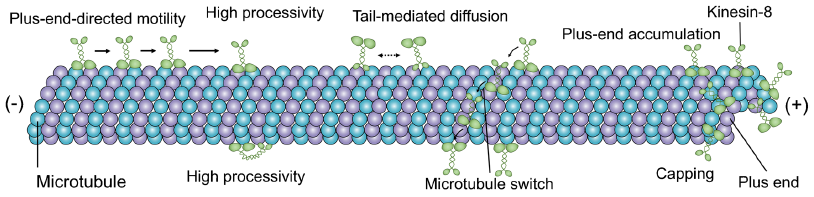
\includegraphics[width=\linewidth]{Figures/kip3.png}
\caption[Introduction to Kinesin-8/Kip3.]{\textbf{Introduction to Kinesin-8/Kip3.}
An illustration of the typical characteristics of members of the Kinesin-8 family, including Kip3. Adapted from \cite{Lin2020}.
	}\label{kip3}
\end{figure}

\subsection{The mitotic spindle}
\label{sec:spindle}
The fission yeast Schizosaccharomyces pombe (S. pombe) is a popular eukaryotic model organism for studying the cell cycle including the mitotic spindle \parencite{Vyas2021, Uzsoy2021}, in part due to its relatively low complexity, as evidenced by its small number of protein-coding genes \parencite{Wood2002}. Other than in animal cells, where the mitotic spindle is established in the cytoplasm, the mitotic spindle of S. pombe forms inside the nucleous \parencite{Kilmartin2014}. As in animals cells, the mitotic spindle allows the cell to separate its two chromosome sets (each containing the DNA for each forthcoming dauther cell) (\autoref{spindle}A).

\begin{figure}[h!tb]
	\centering
	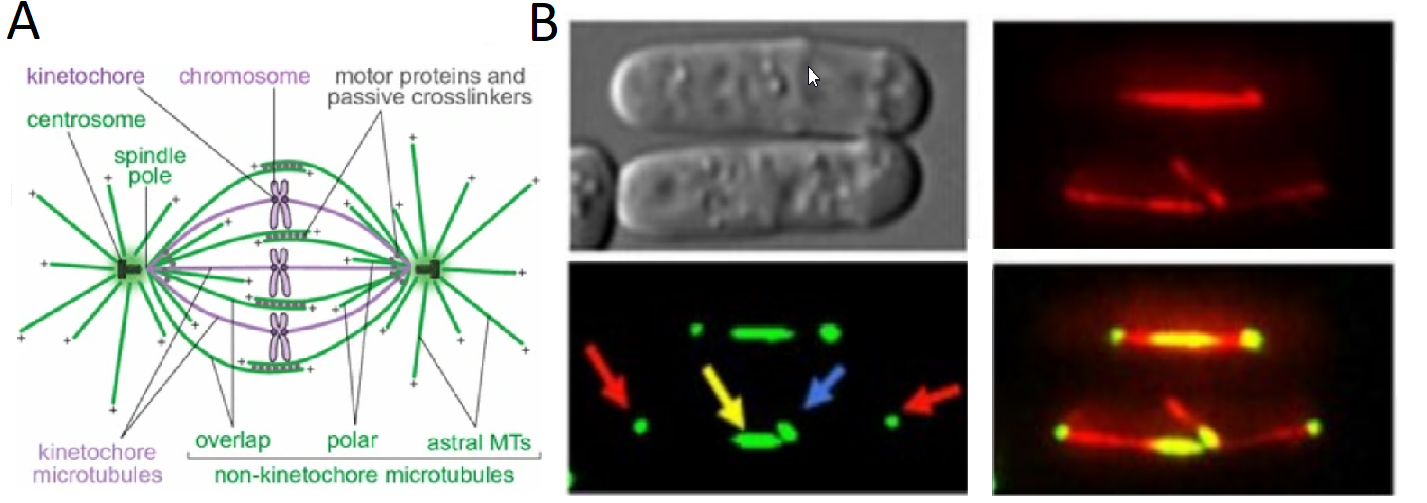
\includegraphics[width=\linewidth]{Figures/spindle.png}
	\caption[Microtubule crosslinkers in the context of the mitotic spindle.]{\textbf{Microtubule crosslinkers in the context of the mitotic spindle.}
	(A) An illustration of the mitotic spindle in animal cells (S. pombe features spindle pole bodies instead of centrosomes, and therefore no astral microtubules \parencite{Kilmartin2014}). The polar microtubules grow from the centrosome, overlapping in an antiparallel fashion in the middle of the nucleous. There, they are crosslinked by passive crosslinkers such as Ase1, but also motor proteins which together with passive crosslinkers contribute to a proper positioning of the mitotic spindle \parencite{Janson2007,Braun2011}. Adapted from \cite{Tolic2018}. The kinetochore microtubules separate the chromosomes from each other and pull them toward the centrosomes (in the next phase of mitosis not shown here). (B) 3D projection images of wild-type S. pombe cells taken during mitosis, with tubulin (CFP-tub1p) in red and Ase1 (Ase1-GFP) in green. Top-left picture taken with differential interference contrast (DIC) microscopy. The yellow arrow indicates the spindle midzone, where Ase1 is binding in between antiparallel microtubule overlaps. Adopted from \cite{Loiodice2005}.
		}\label{spindle}
\end{figure}

\subsubsection{Ase1}
\label{sec:Ase1_intro}
We were interested in the (potential) role of microtubule crosslinkers in building and maintaining the mitotic spindle, where we worked with the S. pombe protein Ase1. Ase1 is a conserved microtubule-bundling protein with orthologues e.g. in plants (MAP65) and mammals (PRC1). During mitosis, Ase1 proteins (or its orthologues in other organisms) are found preferentially at the spindle midzone (\autoref{spindle}B), and are involved in spindle integrity and regulation of spindle elongation \parencite{Loiodice2005,Yamashita2005,She2019}. S. pombe Ase1 deletion mutants, although viable, exhibit interphase microtubules with reduced bundling and mitotic spindles that often fall apart as they elongate in anaphase \parencite{Loiodice2005,Yamashita2005}. \par
Characteristically, the geometry of Ase1 favors antiparallel microtubule arrays, which results in increased Ase1/MAP65/PRC1 affinities for antiparallel microtubule overlaps and preferential antiparallel crosslinking activity \parencite{She2019,Bieling2010,Janson2007,Subramanian2010,Kellogg2016,Gaillard2008}. The preferred binding of Ase1/MAP65/PRC1 family proteins to antiparallel microtubules leads to the recruitment of other proteins that can locally alter microtubule dynamics, such as CLASP \parencite{Bratman2007b,Liu2009,Kitazawa2014} or kinesin-4 \parencite{Bieling2010, Mani2021}. By recruiting these additional factors, Ase1 family proteins can differentially regulate the dynamics of bundled microtubules, specifically affecting the dynamics of antiparallel bundles \parencite{Bieling2010,Bratman2007b, Mani2021}. Additionally, Ase1 family members themselves are also known to have direct effects on microtubule dynamics. In vitro experiments have shown that MAP65-1, upon crosslinking microtubules, promotes rescues \parencite{Stoppin-Mellet2013}. Based on the modeling of their observed overlap dynamics, \cite{Stoppin-Mellet2013} predicted MAP65-1 to have more effect on antiparallel microtubules compared to parallel ones. However, this prediction has not yet been directly experimentally validated.\par
Ase1 possesses a structured N-terminal domain, a central spectrin domain, and an intrinsically disordered C-terminal domain \parencite{Kapitein2008,Kellogg2016}. Ase1 molecules self-associate into homodimers. The N-terminal domain supports this homodimerization and is necessary for microtubule crosslinking activity \parencite{Janson2007}. The spectrin domain and the unstructured C-terminal interact with the microtubule \parencite{Kellogg2016}. Ase1 interacts with microtubules diffusively by exhibiting a one-dimensional random walk along the microtubule lattice. It does so in a "leaping" fashion, where each leap closely matches the tubulin-dimer periodicity, with an approximately twofold higher probability of Ase1 stepping along a given protofilament rather than stepping laterally to an adjacent tubulin dimer of the neighbouring protofilament \pcite{Bujak2021}. When diffusing on a single microtubule, the free microtubule-binding domain samples a large space, allowing for "catching" of another microtubule which subsequently is crosslinked to the first microtubule, preferably in antiparallel fashion (\cite{Janson2007}, \autoref{Ase1}). Within the resulting antiparallel microtubule bundle, Ase1 does still diffuse, albeit with an approximately eight-times lower diffusion coefficient than on single microtubules \parencite{lanskydiffusible2015}.\par
As another feature of Ase1, it has been found that microtubules decorated with Ase1 have a lower flexural rigidity than undecorated microtubules \parencite{Portran2013}.
\begin{figure}[h!tb]
\centering
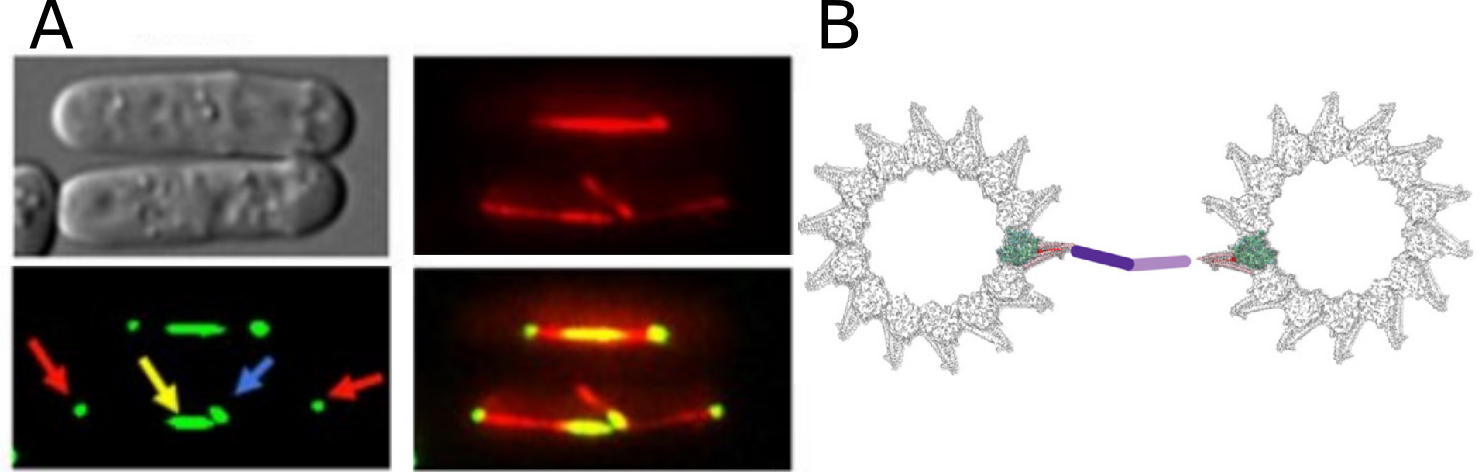
\includegraphics[width=\linewidth]{Figures/Ase1.png}
\caption[Introduction to Ase1.]{
\textbf{Introduction to Ase1.} A model of how PRC1, a Ase1 homologue, binds to two antiparallely aligned microtubules, based on cryo-EM data. The cryo-EM reconstruction is overlayed with shades of green and blue ($\alpha$ and $\beta$-tubulin) and pink (the spectrin domain, the microtubule-binding domain of PRC1 and Ase1). The dimerization domains of PRC1 are shown as cartoons in shades of purple (the cryo-EM study was conducted with a PRC1 construct without the dimerization domain). Adopted from \cite{Kellogg2016}. (A) View from side. (B) Cross section view (from bottom of what panel A shows). 
	}\label{Ase1}
\end{figure}
	\chapter{Aim}
The aim of this thesis and the work underlying it is to further our understanding of the ways in which cytoskeletal polymers, in particular microtubules and microtubule-associated proteins (MAPs) interact to give rise to emergent phenomena. To achieve this, we sought to reconstitute microtubule-based cytoskeletal systems \textit{in vitro} (i.e., outside of biological cells) with a minimal variety of components. This approach can help elucidate which components are needed at a minimum for a given phenomenon to emerge. Moreover, given the low number of confounding factors in such relatively simple assays, it often is possible to gain insights into biophysical mechanisms underlying a given observation. \par
We focused on two different MAPs, aiming to elucidate and potentially recreate phenomena which others had previously observed in the case of \textit{in vivo} cytoskeletal systems in which these MAPs are prominently featured. In both cases, we have a strong focus on the distribution of these MAPs on microtubules and/or microtubules, aiming to contribute to our understanding of how these MAPs may interact with their environment to help spatially organize microtubules within cells. Importantly however, these two MAPs, namely Ase1 and tau (see \autoref{sec:MAPs}), are found in distinct cellular contexts. While Ase1 and its orthologues are primarily involved in mitotic spindle dynamics and cytokinesis, tau is predominantly functioning in the stabilization of axonal microtubules in neurons. Given that they operate under different cellular environments, we have studied these MAPs separately. This separation also reflects the structure of the research publications that form the basis of this thesis, one of which focusing on tau, the other on Ase1 (see \autoref{chap:publications}). To facilitate a clear presentation of the findings presented in these two publications, I have structured the Results section of this thesis accordingly, i.e., it features two separate subsections. Nonetheless, I with this thesis also aim to connect these two parts of my work to the degree to which this is sensible and insightful. This ambition is reflected in the Discussion section, where I aimed to draw insights which go beyond the pecuilarities of each of the two MAPs I was focusing on.
	\chapter{Publications related to this thesis}
\label{publications}
Two publications are related to this thesis, according to which the results part of this thesis is structured.
\section{Publication 1: Kinetically distinct phases of tau on microtubules regulate kinesin motors and severing enzymes}
TODO explanation and author contributions.
This publication can be found in appendix A.
\section{Publication 2: Ase1 selectively increases the lifetime of antiparallel microtubule overlaps}
TODO explanation and author contributions.
This publication can be found in appendix B.
	\chapter{Methods}
\label{methods}

\section{Microtubule preparation}
\subsection{Tubulin preparation}
Tubulin was extracted from pig brains and labeled following previously described methods \parencite{CASTOLDI200383}. Fresh pig brains were cleaned and homogenized in a blender using an ice-cold depolymerization buffer, then centrifuged at 29,000 x g for 60 minutes at 4 ºC. The supernatant was then mixed with an equal volume of high-molarity PIPES, supplemented with 1.5 mM ATP and 0.5 mM GTP, and warmed glycerol at 37 ºC to induce microtubule polymerization. This mixture was incubated for 60 minutes at 37 ºC, followed by centrifugation at 150,000 x g for 30 minutes at 37 ºC. The resulting microtubule pellet was depolymerized by resuspension in ice-cold depolymerization buffer, dounced on ice for 10 minutes, and then incubated for an additional 60 minutes on ice before centrifuging at 70,000 x g for 30 minutes at 4 ºC. Subsequently, the supernatant containing depolymerized tubulin was diluted with equal volumes of prewarmed high-molarity PIPES and glycerol, supplemented with 1.5 mM ATP and 0.5 mM GTP, incubated at 37 ºC for 30 minutes to promote microtubule polymerization, and centrifuged again at 150,000 x g for 30 minutes at 37 ºC. Finally, the microtubule pellet was depolymerized by resuspension in ice-cold BRB80 and dounced on ice for 10 minutes. After an additional 10-minute incubation on ice, the solution was centrifuged at 100,000 x g for 30 minutes at 4 ºC (SW 41Ti rotor). Tubulin was aliquoted, flash-frozen in liquid nitrogen, and stored at -80 ºC for later use. Some tubulin was aliquoted at high concentrations for subsequent labeling (performed by a laboratory assistant), as described by \cite{HYMAN1991478}. Briefly, tubulin labeling involved polymerizing microtubules, incubating them with fluorescent dye, and then depolymerizing the microtubules to obtain labeled tubulin.

\subsection{Microtubule polymerization}
For preparation of biotinylated microtubules, isolated tubulin was mixed with biotinylated tubulin (Cytoskeleton Inc., T333P) at 50:1 mass ratio. For preparation of labeled microtubules, isolated tubulin was mixed with labeled tubulin. We employed two microtubule stabilization techniques \pref{sec:stabilization}{}: i) Polymerizing microtubules under the presence of GMPCPP. ii) Stabilization of microtubules by having paclitaxel present in the buffer \parencite{SCHIFF1979}. GMPCPP-stabilized microtubules were grown using a mixture of 2 $\mu$M tubulin, 1 mM GMPCPP and 4 mM MgCl$_2$ in BRB80 and incubated for 3 hours at 37°C. Paclitaxel-stabilized microtubules were polymerized using a mixture of 1 mM GTP, 4 mM MgCl$_2$ and 5 \% DMSO in BRB80 for 30 minutes and subsequently stabilized by diluting the mixture in BRB80 + 10 µM paclitaxel. In both the GMPCPP and the paclitaxel procedure, the resulting mixture was then spun at 12000 g in a tabletop centrifuge. Finally, the supernatant was discarded, and the pellet was resuspended in 50 $\mu$l BRB80, respectively BRB80 + 10 µM paclitaxel. The paclitaxel-stabilized MTs were not used for assays with dynamic microtubules, as the paclitaxel would cause uninterrupted growth and inhibit catastrophes.

\section{Sample Preparation}
\label{assayPREP}
To conduct our microscopy, we implemented a procedure which has already been described earlier \parencite{Gell2010a}. We manufactured microfluidic channels as depicted in \autoref{Gell2010a_setup}A and after some further preparation steps as described below mounted these channels on the microscope, e.g., for TIRF microscopy as shown in \autoref{Gell2010a_setup}B. The coverslips used in the process, after a cleaning procedure, were functionalized with dichlorodimethylsilane (DDS) to allow for antibody binding to the surface.\par
\begin{figure}[htb]
\centering
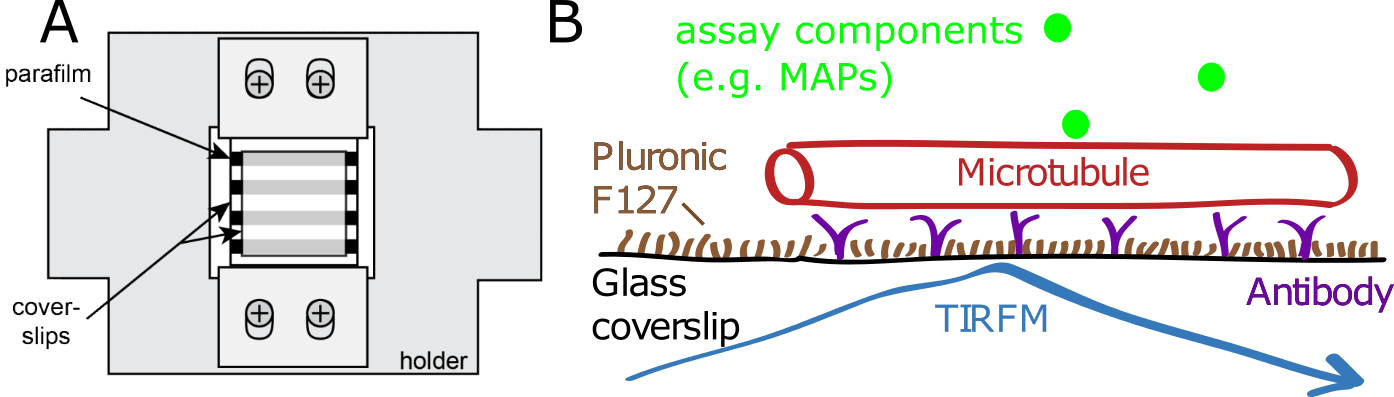
\includegraphics[scale=1.1]{Figures/setup.png}
\caption[The flow cell layout and handling, adapted from \parencite{Gell2010a}.]{
		\textbf{A sketch of the flow cell layout and handling, adapted from \parencite{Gell2010a}}. The four depicted Parafilm stripes were put as spacers in between two DDS-coated glass slides to form three channels. To seal the channels, this construct was then heated up for about 30 seconds while gently pressing the upper slide onto the lower. Next, it was clamped into a brass sample holder. To fill the initially dry channels with liquid, vacuum was employed. Further perfusion steps were conducted by simply utilizing a filter paper as is illustrated. \textbf{B} Schematic of our our experimental setup. The labeling of our microtubules and the included assay components varied from experiment to experiment. 
	}\label{Gell2010a_setup}
\end{figure}
After manufacturing, flow channels were incubated with antibodies in PBS for 1 to 5 minutes (to immobilize biotinylated microtubules, we used anti-biotin antibodies, to immobilize microtubules without biotin, we used anti-$\beta$-tubulin antibodies), followed by incubation for at least 30 min with 1\% pluronic F-127 in PBS to prevent unspecific protein binding. The flow channel was then washed with BRB80 prior to addition of microtubules for antibodyspecific binding ("template MTs"). Unbound microtubules were then removed in another wash step.\par
After these preparatory steps (and in some cases additional steps, see below sections), the assay buffer was added, the flow chambers were sealed in the case of longer experiments to prevent changes in concentrations due to evaporation, and the coverslip holder was mounted onto the microscope stage (setup shown in \autoref{Gell2010a_setup}).

\section{Imaging}
Atto647-labeled microtubules, mCherry- and mEGFP-labeled proteins were visualized sequentially by switching between the Cy5, TRITC and GFP channels (Chroma filter-cubes) using Nikon-Ti E microscope equipped with 100x Nikon TIRF objective and either Hamamatsu Orca Flash 4.0 sCMOS or Andor iXon EMCCD cameras. In the case of tau experiments, the acquisition rate varied between 1 frame per 30 ms to 1 frame per 30 seconds depending on the particular experiment and is indicated in the corresponding figure. In the case of one set of Ase1 experiments (Set A, see \autoref{Ase1AssayMethods}), the GFP channel was visualized or the IRM channel (or both with sequential switching), at a framerate of 5s. For the other set of Ase1 experiments (Set B), channels were sequentially switched at a framerate of 2.6 seconds (with a 633x Zeiss oil immersion TIRF objective in combination with a Andor iXon DV 897 (Andor Technology) EMCCD camera). Imaging conditions in experiments used for quantitative estimation of kinetic parameters were set such that photo-bleaching effects were negligible (< 2 \% fluorescent intensity loss during the experiment). Finally, for Ase1 Set A experiments, the Alexa647-labeled MT seeds were imaged before the start of the time lapse, and only the Ase1-mNeonGreen channel was imaged during the time lapse. For Set B experiments, the rhodamine (tubulin) and the GFP (Ase1-GFP) channel where imaged sequentially, whereas every 40th frame the Alexa647 channel was imaged in place of the GFP channel, in order to track the location of the GMPCPP-stabilized seeds (which we with this data determined to not move significantly during experiment time). 

\section{Image analysis}
\label{methods_analysis}
Data was analyzed using FIJI \parencite{Schindelin2012} and custom written Matlab (Mathworks) routines. 
\subsection{Density estimation}
Kymographs (KymographBuilder plugin, custom-modified to compute integrated intensity instead of finding the maximum intensity, see Zenodo: \url{doi.org/10.5281/zenodo.3270572}) along the microtubule length were used to read out the fluorescent signal and to estimate the integrated signal intensity of fluorescent proteins bound to the microtubule (if necessary, time series were drift-corrected with FIESTA \parencite{RUHNOW20112820}). The recorded signal in regions directly adjacent to the microtubule was subtracted as background signal. Kymograph pixels were then manually categorized according to the type of microtubule region they covered (island, curved microtubule, regions surrounding the islands in case of tau, overlapping microtubules or single microtubules in the case of Ase1). The integrated intensity averaged along the microtubule length for each region type was then computed by taking the mean of the categorized kymograph pixels (in the case the Ase1 assays, only regions with dynamic extensions present were measured). The density of labeled MAPs bound to the microtubule was then estimated by dividing the averaged integrated intensity by estimated intensity per single molecule times unit length. Conversion to the number of MAP molecules per tubulin dimer was performed assuming 13 available protofilaments and 8 nm length of a tubulin dimer.

\subsection{Diffusion coefficient estimation} 
Single tau molecule tracking for the estimation of diffusion coefficients (TODO, \aref{ase2FRAP}{B}) was performed using FIESTA\parencite{RUHNOW20112820} software. For reconnecting tracks, a threshold velocity of 12000 nm/s had been chosen, and tracks were allowed to have at most 3 missing frames between two data points. To minimize false-positive connecting of separate molecules, the tracks obtained by FIESTA were cut into pieces such that the maximum distance between two data points was never above 360 nm.

\subsection{Fluorescent signal of a single fluorescent molecule} 
In our assays, we often were interested in the absolute number of labeled proteins bound to microtubules. To estimate this number, it was necessary to know the contribution of single fluorophores to the measured signal. The fluorescent signal of a single fluorescent molecule was determined by generating intensity time-traces of single fluorophore-labeled kinesin-1 molecules tightly bound to the microtubule in presence of AMP-PNP (in the absence of ATP) and estimating the height of the occurring bleaching steps. The number of steps was first estimated by eye, and this number was used as input for the \textit{findchangepoints} function of Matlab to determine the position of the steps (see \autoref{bleaching_steps}). To yield the intensity per single molecule, the heights of these steps were averaged (and in the case of Ase1, multiplied by two, given that Ase1 forms homodimers).
\begin{figure}[htb]
\centering
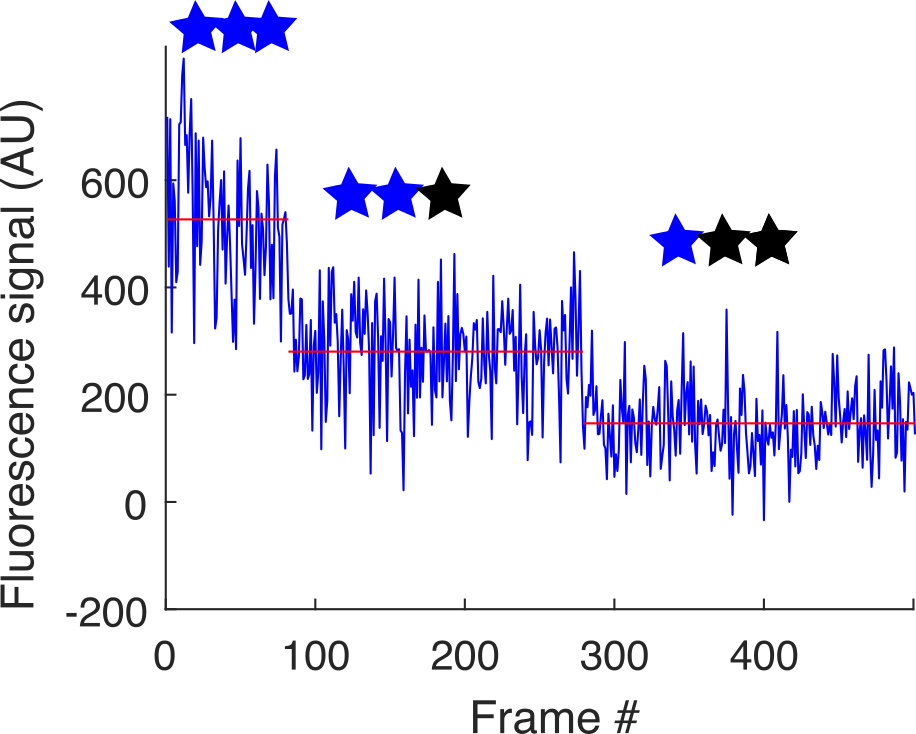
\includegraphics[scale=1.1]{Figures/bleaching_steps.png}
\caption[An illustration explaining our estimation of the fluorescent signal of a single fluorophore.]{\textbf{An illustration explaining our estimation of the fluorescent signal of a single fluorophore.}
		The signal recorded on a particular spot on a microtubule decorated with immobilized fluorophore-labeled kinesin-1 molecules. The signal shows a step-wise decay due to photobleaching of the fluorophores. The bleaching steps were detected detection of significant changes of the mean values.
	}\label{bleaching_steps}
\end{figure}

\section{Data representation}
In all boxplots presented in the figures, horizontal midline indicates the median; bottom and top box edges indicate the 25th and 75th percentiles, respectively; the whiskers extend to the most extreme data points not considered as outliers (the function Alternative box plot from the IoSR Matlab Toolbox has been used); the numbers indicate the sample size; the notches are centered on the median and extend to ±1.58*IQR/sqrt(sample size). Where single, colored data points are presented, points from the same experiment are indicated by the same color (unless otherwise stated). 

\section{Procedures specific to tau experiments}
\subsection{Protein expression and purification} 
mEGFP or mCherry tagged tau and tau$\Delta$N, Kinesin-1, Kip3 and katanin (M. musculus katanin p60/p80C, \cite{Jiang2017}) were expressed and purified as described previously \parencite{HERNANDEZVEGA20172304,Herrmann2018,Mitra2018,NITZSCHE2010247}. In particular, all tau variants \pref{tauconstructs}{} were purified from insect cells using the baculovirus expression system. Recombinant baculovirus for each construct was produced as described by \cite{woodruff2015method}. Sf9 insect cells in log phase (1 million cells/ml, Expression system) were infected with 5 ml of P2 baculovirus stock, incubated at 27°C with moderate shaking, and harvested 72 hours post-infection. The cells were collected by centrifugation at 700g for 8 minutes and then resuspended in resuspension buffer [25 mM HEPES, 150 mM KCl, 20 mM imidazole (pH 7.4) with 1 mM DTT, 1 mM PMSF (Sigma), and 1x Protease Inhibitors Cocktail (Calbiochem, Type III)]. Cell lysis was performed using an Emulsiflex (Emulsiflex-C5, Avestin). The lysate was centrifuged at 35,000 rpm for 45 minutes, and the supernatant was collected. The supernatant was filtered through a 0.45 µm filter and incubated with Ni-NTA agarose resin (QIAGEN) HiTrap for 1 hour. The beads were collected and washed using disposable gravity columns (20 mL, Biorad). The columns were washed four times with 20 ml of wash buffer (25 mM HEPES, 150 mM KCl, 30 mM imidazole, 1 mM DTT, pH 7.4) and eluted with an elution buffer (same buffer containing 250 mM imidazole). The 6xHis tag was removed by treatment with PreScission protease (3C HRV protease, 1:100, 1 µg enzyme/100 µg of protein) overnight at 4°C. Imidazole was removed by dialysis (slide-a-lyzer with a 20 KDa cut-off) overnight at 4°C, with His tag cleavage occurring simultaneously with dialysis. The protein was further purified by size-exclusion chromatography using a HiLoad 16/60 Superdex 200 column with an ÄKTA Pure Chromatography system (GE Healthcare) in 25 mM HEPES, 150 mM KCl, 1 mM DTT (pH 7.4). Collected peak fractions were concentrated to 100 µM or 200 µM using Amicon Ultra 30K (Millipore). Protein concentration was measured using a NanoDrop ND-1000 spectrophotometer (Thermo Scientific) at 280 nm absorbance. Proteins were flash-frozen in liquid nitrogen and stored at -80°C. All steps in the purification were performed at 4°C. 

\begin{figure}[h]
	\centering
	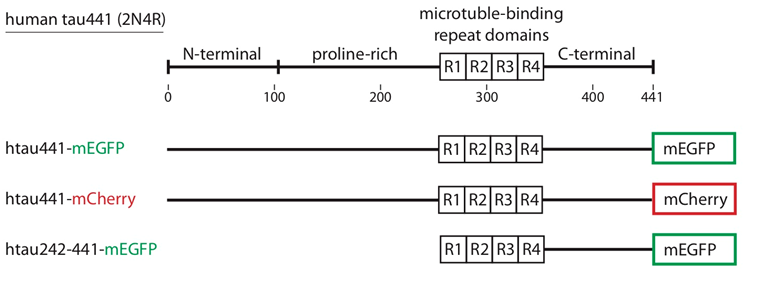
\includegraphics[width=0.6\linewidth]{Figures/tauconstructs.png}
	\caption[Schematics showing the tau constructs used in this study.]{
		\textbf{Schematics showing the tau constructs used in this study.}
		}\label{tauconstructs}
\end{figure}

\subsection{In vitro tau-microtubule binding assay}
Biotinylated, paclitaxel-stabilized, Atto647-labeled microtubules in BRB80T (80 mM Pipes/KOH pH 6.9, 1 mM MgCl2, 1 mM EGTA, 10 µM paclitaxel) were immobilized in a flow chamber using biotin antibodies \pref{assayPREP}{}. Subsequently, assay buffer was flushed into the flow cell (20 mM HEPES pH 7.2, 1 mM EGTA, 75 mM KCl (unless stated otherwise in the main text), 2 mM MgCl2, 1 mM ATP (+Mg), 10 mM dithiothreitol, 0.02 mg/ml casein, 10 µM paclitaxel, 20 mM d-glucose, 0.22 mg/ml glucose oxidase and 20 µg/ml catalase). Then, tau in assay buffer was flushed in at the final assay concentration stated in the main text. In experiments involving multiple successive tau additions, the flow cell was rinsed between each tau addition with a high ionic strength buffer (200 mM KCl in addition to the assay buffer). To remove tau from the solution, the chamber was perfused with approximately four times the chamber volume using assay buffer without tau. For high tau concentrations (>200 nM), larger volumes (up to ten times the chamber volume) were used to ensure complete removal of tau. In experiments with kinesin-8, katanin, or kinesin-1, islands were preformed before introducing the respective protein into the solution, while maintaining a constant tau concentration. In the katanin experiment with elevated tau concentration (see \aref{taukatanin}{}), microtubules were first incubated with 0.8 µM tau-mCherry for 5 minutes. Tau-mCherry was then temporarily removed from the measurement chamber for less than 1 minute to identify the position of the islands, which were obscured by the high tau-mCherry density in the surrounding areas. Tau-mCherry was then reintroduced at 0.8 µM, and after 5 minutes, 215 nM katanin-GFP was added to the solution, while maintaining the tau concentration at 0.8 µM. All experiments were conducted at room temperature.


\subsection{Coverage by tau islands}
The proportion of microtubule length occupied by tau islands was determined by representing both islands and microtubules as segmented lines, measuring their respective lengths, and then calculating the ratio of the total island length on a given microtubule (or within a field of view) to the length of that microtubule (or the combined length of all microtubules in the field of view).

\subsection{Estimation of velocities}
The rates of assembly and disassembly of island boundaries (in the absence or presence of katanin or Kip3) were determined by fitting straight lines to the advancing or retreating edges of tau islands in kymographs. The velocity provided in the text represents a duration-weighted average of these segments. To convert this velocity to the number of tau molecules per second, it was multiplied by the estimated density of tau within the islands (in molecules per nanometer), assuming tau binds to 13 protofilaments with a tubulin dimer length of 8 nm. The velocities of Kip3 and kinesin-1 were determined by fitting straight lines to the kymographs of the moving motors, both inside and outside the islands.

\subsection{Estimation of the tau unbinding time}
To determine the unbinding times of tau inside and outside the islands, the decay in tau density over time was analyzed after a buffer exchange either removing tau from the solution or replacing tau-mEGFP with tau-mCherry. Each analyzed region (island or surrounding area) provided a time trace of tau density decay following the buffer exchange. Time traces from representative experiments were combined, as shown in \aref{tauSHRINK}{E,F}, with the thick line representing the median of all traces at each time point and the bounds showing the first and third quartiles. To estimate the mean residence times of tau inside and outside the islands, individual density time traces were fitted with an exponential decay using the Matlab function fit, excluding data points before the solution exchange. The fits and mean residence times presented were calculated by averaging the coefficients from the individual fits.

\subsection{Katanin severing rate estimation}
Severing rates in regions surrounding the islands were determined by fitting an exponential decay to the number of pixels corresponding to the original microtubule position that exceeded a manually set threshold, which encompassed the microtubule. In island regions, the severing events were counted. In \aref{taukatanin}{B}, the estimated severing rates include both straight and curved microtubules. In \aref{taucurve}{H}, the severing rates are categorized based on the following criteria: straight microtubules were defined as stretches where the orientation did not change by more than 10 degrees, while curved regions were defined as 0.5 µm long stretches centered at the point of greatest curvature with a radius of less than 2.5 µm.

\section{Procedures specific to Ase1 experiments}
\subsection{Protein expression and purification}
Ase1-GFP \parencite{Janson2007} and Ase1-mNeonGreen were expressed in E. coli strain BL21 (DE3) (Altium International). After harvesting the cells, the cell pellet was resuspended in 5 mL ice-cold phosphate buffered saline (PBS) and stored at -80°C for further use. For cell lysis, the cells were homogenized in 30 mL of ice-cold His-Trap buffer (50 mM Na-phosphate buffer, pH 7.5, 5\% glycerol, 300 mM KCl, 1 mM MgCl2, 0.1\% Tween 20, 10 mM BME, 0.1 mM ATP) supplemented with 30 mM imidazole, Protease Inhibitor Cocktail (cOmplete, EDTA free, Roche), and benzonase (Novagen) at a final concentration of 25 units/mL. The mixture was then sonicated and subsequently centrifuged at 45,000 x g for 60 minutes at 4°C using an Avanti J-26S ultracentrifuge (JA-30.50Ti rotor, Beckman Coulter). The clarified cell lysate was incubated with Ni-NTA resin (HisPur Ni-NTA Superflow Agarose, Thermo Scientific) pre-equilibrated with lysis buffer for 2 hours at 4°C. The resin was then sequentially washed with wash buffer I (His-Trap buffer with 60 mM imidazole) and wash buffer II (His-Trap buffer with 60 mM imidazole and 700 mM NaCl). Ase1-GFP was eluted using His-Trap buffer supplemented with 300 mM imidazole. For Ase1-mNeonGreen, after the second wash with buffer II, the resin was further washed with wash buffer I containing 3C PreScission protease (Merck Millipore), which cleaved Ase1-mNeonGreen from the column at the 3C protease cleavage site between mNeonGreen and the 6xHis-tag (the Ase1-mNeonGreen construct had been created by Lenka Grycova). The mixture was incubated overnight at 4°C. The following day, the beads were removed, and the cleaved protein was collected. Both Ase1-GFP and Ase1-mNeonGreen were concentrated by centrifugation at 3500 RPM at 4°C using a 100 kDa centrifugal filter tube (Amicon Ultra-15, Merck). Ase1-mNeonGreen underwent a second purification step through size exclusion chromatography using a Superdex 200 10/300 column. The size exclusion buffer consisted of 100 mM Tris, 150 mM NaCl, 1 mM MgCl2, 1 mM DTT, 0.05\% Tween, 0.1 mM ATP, and 10\% glycerol. Fractions containing the protein were collected and concentrated. The final protein concentrations were measured with a NanoDrop ND-1000 spectrophotometer (Thermo Scientific) at absorbances of 280 and 506 nm. The protein was flash-frozen in liquid nitrogen and stored at -80°C. All purification steps were performed at 4°C.

\subsection{In vitro Ase1-microtubule binding assay}
\label{Ase1AssayMethods}
Biotinylated, GMPCPP-stabilized, fluorescence-labeled MTs in BRB80 (80 mM Pipes/KOH pH 6.9, 1 mM MgCl2, 1 mM EGTA) were flushed into the prepared channels, were given time to bind to biotin antibodies, and were removed from solution, as described in \autoref{assayPREP}. In the case of Ase1 Set B experiments, additional preparatory steps occured: First, a buffered solution with a low concentration of Ase1 was flushed in, Ase1 was allowed to sparsely bind to the template MTs, removed from solution, and subsequently non-biotinylated GMPCPP-stabilized MTs were flushed into the flow cell which got crosslinked to the template MTs by the Ase1 on these MTs. These MTs were labelled with both rhodamine and Alexa647 (represented in sketches in dark blue), while the templates in these assays were only very weakly labelled with Alexa646 (represented in sketches in light blue). Then, the "transport" MTs were removed from solution so that only transports which formed overlaps with templates would remain in the channel. \par 
The buffer in the flow cell was then exchanged for assay buffer. Finally, Ase1 in assay buffer was flushed into the flow cell at the final assay concentration stated in the main text, together with tubulin, and the channels were sealed. Set A experiments (shown in Figures \ref{ase1a}, \ref{ase1b}, \ref{ase1c}A-E, \ref{ase1d} and \ref{ase2a}) were performed at room temperature and with 32$\mu$M unlabeled tubulin present in solution. Set B experiments (shown in Figures \ref{ase1e}, \ref{ase2b}, \ref{ase2c}C,D and \ref{ase2e}) were performed at 29°C and with 14$\mu$M tubulin, 7\% of which was labeled with rhodamine. The following buffer components common to all used buffers in experiments involving Ase1: 20mM PIPES pH 6.9, 10mM HEPES pH 7.2, 0.5mM EGTA, 1mM MgCl2, 0.5mM Mg-ATP, 0.67mM GTP, 0.67\% Tween20, 6.7mM DTT, 0.3 mg/ml Casein, 13.5mM D-Glucose, 0.3mg/ml glucose oxidase and 0.03mg/ml catalase. The buffer for Set A experiments, in addition to these components, contained 70mM KCl, and 0.1\% Methylcellulose, 0.1\% Glycerol, 1mM sodium phosphate and 1µM ATP. The buffer for Figure Set B experiments, in addition to the components common to all buffers, contained 116mM KCl and 0.065\% Methylcellulose. Experiments shown in Figures \ref{ase1c}F and \ref{ase2c}A,B were performed at the same experimental conditions as Set A experiments (with small differences dependent on the particular experiment as stated in the main text/figure captions).

\subsection{Estimating Overlap Lifetime}
The lifespan of microtubule overlap regions was determined for two distinct microtubule configurations: Antiparallel "midzones," where two dynamic extensions converged to form a dynamic midzone (as depicted in \aref{ase1a}{ left panel}), and parallel bundles composed of two dynamic extensions (as shown in \aref{ase1a}{ right panel}). In both cases, whether antiparallel midzones or parallel bundles, the lifetime was considered to begin when the dynamic (GDP) lattices of each participating microtubule were crosslinked (for antiparallel configurations, an additional condition was that both plus ends had to be within 3 microns of each other at the event's start) and ended when one of the microtubules depolymerized back to its GMPCPP-stabilized segment. For antiparallel bundles, the lifetime also concluded when the midzone was no longer present. If an overlap region persisted until the time-lapse movie concluded, the event was classified as censored. \aref{ase1a}{A} and \aref{ase1c}{B} were created using the Matlab function ecdf with the “survival” option enabled.

\subsection{Adjustment for Ase1 Signal Measurement}
To measure the equilibrium density of Ase1, the signal per unit length (S) detected on isolated microtubules was used to adjust for the reduced illumination intensity in the outer regions of the field of view (when a region of interest (ROI) was located in those regions): $S_{\textrm{corrected}}(ROI) = S(ROI) * S(\textrm{isolated MT in center of field of view}) / S(\textrm{isolated MT near ROI})$.

\subsection{Determining Microtubule Dynamic Instability Parameters}
The parameters of microtubule dynamics for Set A experiments were estimated by generating kymographs and fitting straight lines to track the position of microtubule plus ends over time and space (using the Ase1-mNeonGreen signal to visually track MT ends, as microtubules were not directly imaged). For Set B experiments, the FIESTA software was employed to pinpoint the locations of microtubules \parencite{RUHNOW20112820}. Both methods provided measurements of polymerization and depolymerization velocities. Rescues were identified as instances where a microtubule transitioned from depolymerization to polymerization before reaching the GMPCPP-stabilized seed, while catastrophes were noted when polymerization switched to depolymerization. The frequencies of rescues and catastrophes were calculated by dividing the number of rescues and catastrophes by the total distance depolymerized and polymerized by all plus ends, respectively. In the case of Set A experiments, we tested 10nM during the revision phase, a time when room temperatures were less stable. Consequently, microtubule velocities at all Ase1 concentrations differed from our initial experiments. To allow pooling these results with our initial data, we adjusted the velocities from these experiments by multiplying them by a factor calculated as follows: The mean polymerization and depolymerization velocity of isolated microtubules at 42nM from the initial experiments was divided by the mean respective velocity of isolated microtubules at 42nM from the revision-phase experiments (these mean velocities were weighted by the duration of each polymerization or depolymerization event). The resulting adjustment factors were 0.4 for polymerization and 0.39 for depolymerization.

\subsection{Estimation of amount of Ase1 being swept}
To estimate the number of swept Ase1 molecules for corresponding panels in \aref{ase2b}{} (Set B experiments), we first obtained density traces for each frame during a MT depolymerization period. These traces were obtained by summing the pixel intensities perpendicular to the MT, i.e., by generating kymograph where each pixel represents such a sum (\url{doi.org/10.5281/zenodo.3270572}). For each frame f we analyzed the corresponding density trace $D_f$ as follows. (1) We computed $D_s$ by subtracting the density trace $D_{before\_catastrophe}$ of the MT before the catastrophe had occurred from $D_f$ ($D_s = D_f - D_{before_catastrophe}$) (2) We obtained $x = 0 = X_{Dsmax}$, the location of the local maximum of $D_s$ in vicinity of the MT plus end. (3) We obtained $X_{Dsright}$ by finding the first local minimum of $D_s$ to the right of $X_{Dsright}$ (to reduce the effect of noise, we smoothed $D_s$ for this computation). “Right” of $D_s$, in the here-chosen coordinate system, means toward the MT seed ($x > 0$). (4) $X_{Dsleft} = X_{Dsmax} -$ 471nm (471 nm = 3 pixels). (5) We computed $D_A$. $D_A$ is equal to $D_f$ to the left of $X_{Dsmax}$, and equal to $D_s + Df(X_{Dsmax}) - D_s(X_{Dsmax})$ to the right of $X_{Dsmax}$. (6) We fitted a distribution $Y_F$ (shape see below) plus an error function $Y_E$ to $D_A$ between XDsleft and $X_{Dsright}$. We required both $Y_F$ and the error function to not have any x-offset: $Y_F$ was a right-sided decaying exponential $exp^{-x/\sigma}$ ($Y_F = 0$ where $x < 0$, and with $\lambda$ bounded between 1 and 1000 nm) convolved with a gaussian $exp^{-x2/2\sigma2}$ (with $\sigma$ bounded between 180 to 190 nm to account for the point spread function of our setup; this same $\sigma$ had been used as input for $Y_E$). Instead of a blurred right-sided decaying exponential, we for some fits (shown in \aref{ase2e}{}) used a gaussian $exp^{-x2/2\sigma_G2}$ for $Y_F$ (with a $\sigma_G$ between 180 nm and 450 nm, which was independent of the $\sigma$ used for blurring $Y_F$). We also fixed $G+E$ (plus a constant value) to approach the minimum of $D_A$ to the left of the end, and the average of $D_A$ to the right of $X_{Dsright}$ (the average of $D_A$ within 5 microns from $X_{Dsright}$, giving more weight to values close to $X_{Dsright}$). (6) We then summed the Ase1 density below $Y_F$ (as discretized in x by the pixel size), which we took as a proxy for the number of swept Ase1-GFP molecules after dividing by the intensity per Ase1 dimer (obtained as described above). 

\subsection{Fluorescence recovery after photobleaching (FRAP)}
Biotinylated GMPCPP-stabilized MTs were immobilized on the coverslip. We then flushed in the same assay buffer as for Set A experiments, incubated until the Ase1 density on MTs reached a steady-state, and subsequently bleached Ase1-mNeonGreen molecules and recorded the recovering Ase1-mNeonGreen signal. We fitted the resulting recovery curve to the expression $D_s - c exp(-bt)$, where $D_s$ is the steady state density, and $c$ and $b$ are fitting parameters (see \aref{sec:FRAP}{}). Results for fitting parameter $b$ are shown in Figure S4D.

\subsection{Mathematical modelling}
The scripts to reproduce the modelling, and to plot experimental and theoretical results from \aref{ase2d}{} and \aref{ase2steady}{} can be found in Zenodo: \url{doi.org/10.5281/zenodo.12169420}. 
\subsubsection{Assumptions}
The model of Ase1 accumulation on depolymerizing MTs, and its effect on depolymerization velocity \pref{ase2d}{A} is built on the following assumptions:
\begin{enumerate}
	\item We neglect interactions between protofilaments and only consider a one-dimensional lattice, where lattice of size $a=8$nm start at index $i=1$ at the plus end, extending to $i=400$. 
	\item Only bound Ase1 molecules are considered by recording the presence or absence (0 or 1) of Ase1 in each lattice site. Bound Ase1 molecules exchange with solution with two constant rates ($k_{on},k_{off}$). Binding is only allowed if the lattice site is empty \pref{ase2d}{A}. $k_{off}$ was directly measured, and $k_{on}$ was adjusted to match the Ase1 equilibrium density on MTs \pref{ase2t1}{}.
	\item Ase1 particles on the lattice undergo unbiased diffusion characterized by a constant hopping rate ($k_h$). Hopping is only allowed to an empty site \pref{ase2d}{A}. The rate $k_h$ is calculated from the experimentally measured diffusion coefficient of Ase1 \pref{ase2t1}{}, as $k_h=D/a^2$.
	\item The Ase1 particle in the terminal site ($i=1$), cannot hop past the MT end (red arrow on the left of \aref{ase2d}{A}), but can detach with rate $k_{off}$.
	\item The terminal lattice site may dissociate from the MT, with rate $k_d$ which depends on the presence of Ase1, according to each model:
	\begin{enumerate}
		\item In Model 1, it occurs with rate $k_d^0$ if the terminal lattice site is not occupied \pref{ase2d}{B, top}, and with rate $(1-\Omega)k_d^0$ if it is occupied \pref{ase2d}{B, bottom}. $\Omega$ is a parameter between zero and one. If $\Omega=0$, the presence of Ase1 has no effect, and if $\Omega=1$, the first tubulin subunit cannot unbind if it is bound to Ase1.
		\item In Model 2, the rate of tubulin subunits loss at the plus end is reduced by a factor ($1-\Omega$) if any of the N terminal sites is occupied. At steady state, this rate is $k_d=k_0^d [1-\Omega(1-\prod_{i=1}^{i=N}(1-P_i))]$, where $P_i$ is the probability of site $i$ being occupied by Ase1.
	\end{enumerate} 
	$k_d^0$ is derived from the depolymerization rate of MTs in the absence of Ase1 ($v_0$), measured experimentally \pref{ase2t1}{}, such that  $k_d^0=v_0/a$.
	\item If the terminal lattice site dissociates when a molecule of Ase1 is bound to it, this Ase1 is lost as well \pref{ase2d}{B, bottom}.
\end{enumerate}
	
\subsubsection{Simplification to a system of constant size}
Since terminal subunits are more likely to be lost when they are without Ase1 than when they are with Ase1, any dissociation event increases the density of Ase1 remaining on the MT. This effect is only present at the MT end, and away from the end, the probability of a binding site being occupied is only determined by the binding and unbinding constants: $\alpha=k_{on}/(k_{on}+k_{off})$.
Therefore, we can restrict the model to a section of the MT with $L$ lattice sites, as long as the probability of finding a molecule at position $L$ is close to $\alpha$. When a depolymerisation event happens, we shift the lattice indexes such that site $i+1$ becomes site $i$, and set $P_{i=L}= \alpha$. 

\subsubsection{Mean field theory}
The system can be solved using a mean-field approximation, by just considering the ensemble of  $P_i$, the average probability of a site i being occupied and neglecting higher-order correlations between neighbouring sites. We can then write a set of discrete differential equations to represent the dynamics of the system:
\begin{equation}
	\frac{dP_i}{dt}=(P_{i+1}+P_{i-1}-2P_i ) k_h+(1-P_i ) k_{on}-P_i k_{off}+(P_{i+1}-P_i ) k_d
\end{equation}

Specific equations apply at the boundaries $i=1$ and $L$:
\begin{align}
	\frac{dP_1}{dt} &= k_h (P_2-P_1 )-P_1 k_{off}+(1-P_1 ) k_{on}+k_d P_2-k_d^0 P_1 (1-\Omega) \\
	dP_L/dt &= 0
\end{align}

The terms of the equation are associated with the rates of diffusion, binding, unbinding ($k_h,k_(on ),k_{off}$) which are constant, and the depolymerization rate ($k_d$), which is affected by lattice occupancy in a different way in each model (see Assumptions).\\
For Model 1, $k_d=k_d^0 (1-\Omega P_1)$.\\
For Model 2, $k_d=k_d^0 [1-\Omega+\Omega\prod_{i=1}^{i=N}(1-P_i)]$.\\
This dynamical system can be evolved from any initial conditions, converging to the unique steady-state solution for a set of given parameters. Assuming that the MT is at binding equilibrium when it starts depolymerizing, we initially set $P_i=\alpha$ for all sites. From those initial conditions, we integrate the equations numerically using Python’s \textit{odeint} function (see source code).

\subsubsection{Modelling of overlaps}
To model MT overlaps \pref{ase2d}{E,G}, we assume that the Ase1 measured in the overlaps (see Image Analysis above) is evenly distributed among 3 protofilaments that are involved in crosslinking the MTs. We neglect the other protofilaments. We had also modelled 2 protofilaments instead of 3, which did not fit the experimental data as well as 3 protofilaments.

\subsection{Comparison of experimental data and model}
To compare the predicted and observed timescale of Ase1 accumulation ($\tau$) and Ase1 accumulation at steady state ($A_{end}$), the accumulated Ase1 as a function of time was fitted to $A_{end} (1-exp^{-t/\tau})$ in experiments and model predictions (e.g., \aref{ase2d}{F} for isolated MTs at 6nM of Ase1). In the model, the accumulation of Ase1 at any given timepoint is defined as $(\sum_{i=0}^{i=L}Pi)-\alpha L$. As a proxy of velocity of depolymerization at steady state, we used the average velocity of depolymerization observed after 20 seconds of depolymerization in experiments and compared it to the depolymerization velocity at the last simulated timepoint \pref{ase2d}{F}. The 95\% confidence intervals of these magnitudes were estimated using the bootstrap method. For each experimental condition with N depolymerization events, a thousand sets of N depolymerization events were drawn through sample with replacement. For each of those sets, $\tau$ and $A_{end}$ were calculated by fitting all observations in the set, and the average velocity after 20 seconds was calculated. Then, the distribution of each magnitude across all sets was used to calculate the 95\% confidence intervals (see source code).

	\chapter{Results}
	\section{Interactions of distinct phases of tau with other MAPs}
\label{sec:tau}
\subsection{Tau has one diffusive and one cooperative microtubule binding mode}
\captionsetup[<float-type>]{list=no}
\begin{figure}[b!]
\centering
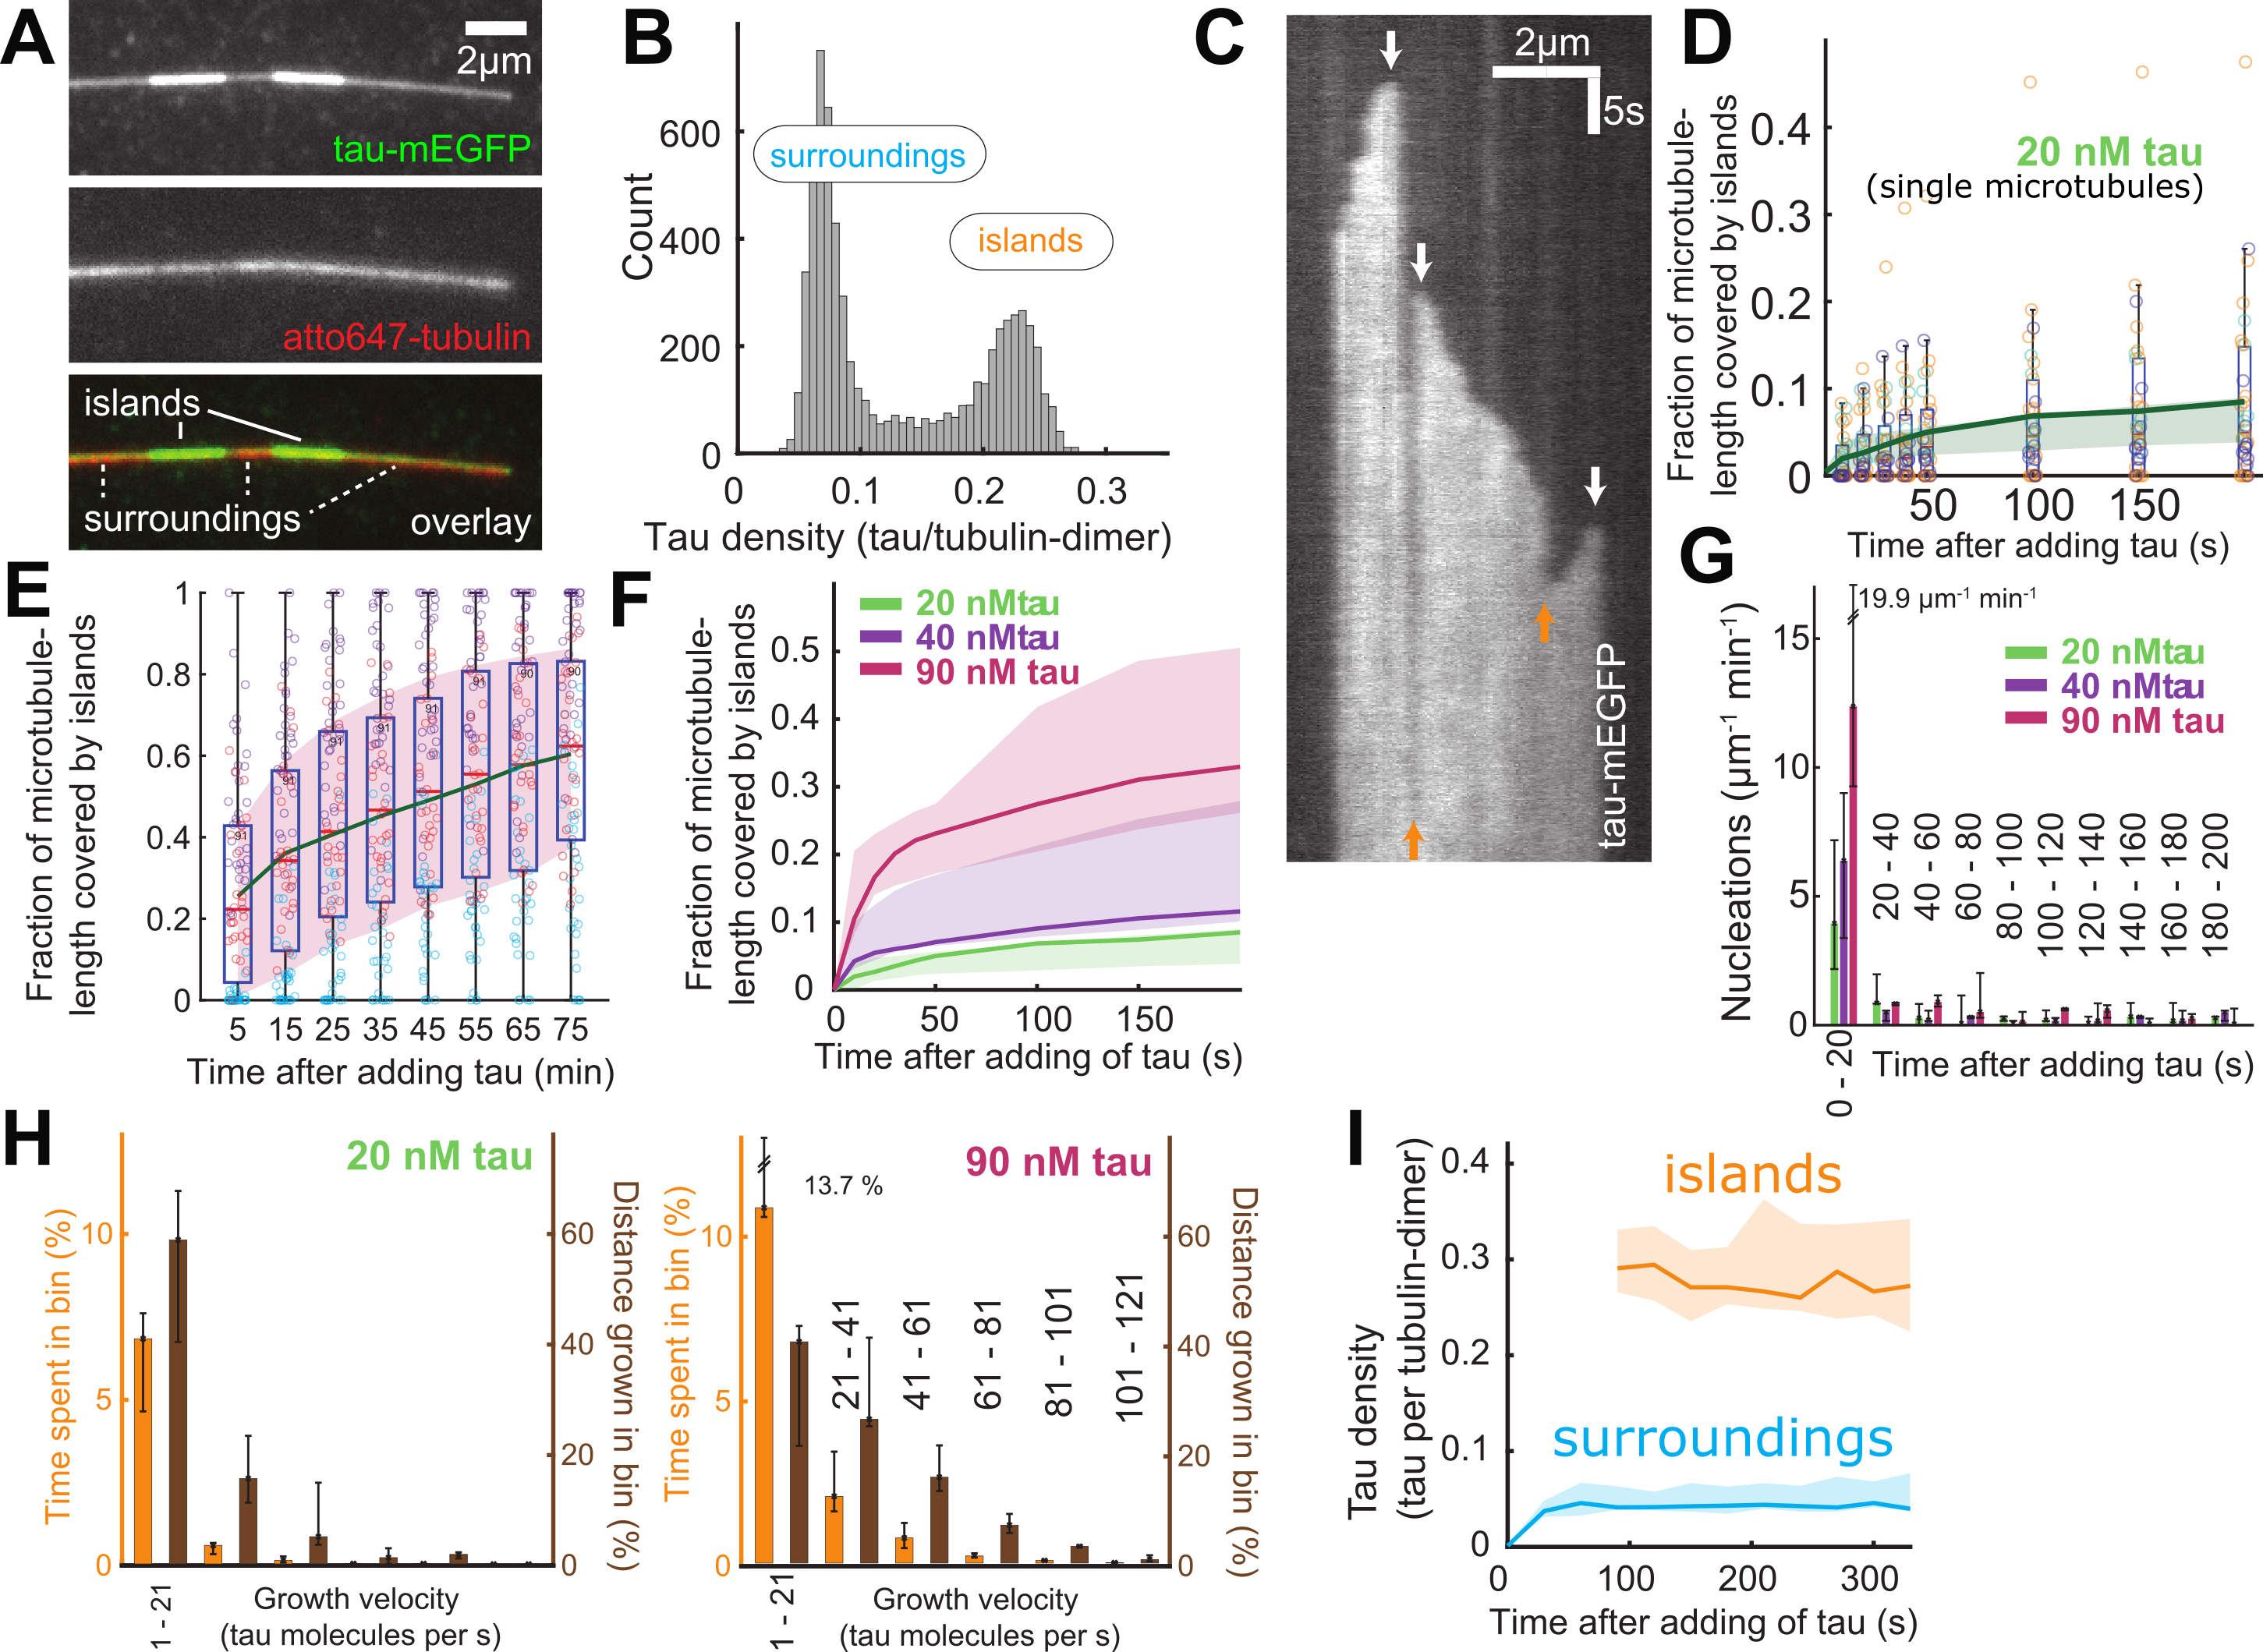
\includegraphics[width=1\linewidth]{Figures/tauGROW.png}
\end{figure}
\captionsetup[<float-type>]{list=yes}
\begin{figure}[t!]
\caption[Tau assembles into tau islands on microtubules.]{\textbf{Tau assembles into tau islands on microtubules.} (A) Multichannel fluorescence micrograph showing areas of high-density tau (bright green) surrounded by regions of low-density tau (dim green) on an Atto-647-labeled microtubule (red). Images taken 5 minutes after adding 20 nM tau. (B) Distribution of fluorescence intensity of tau along the microtubules such as shown in A showing two distinct populations. (C) Kymograph showing the fluorescence signal of tau on a microtubule after the addition 20 nM tau. Initially the microtubule is covered by low tau density. Over time, high-density regions ("islands") start to assemble. White arrows indicate the nucleation points; orange arrows indicate the merging of two neighboring islands growing towards each other. (D) Fraction of microtubule length covered by tau islands at different concentrations after adding tau at time = 0 (n = 3 experiments, shaded area is drawn between the experiment with least coverage and experiment with most coverage, line shows coverage in remaining experiment). Boxplots represent the coverage statistics of individual microtubules. (E) The same data representation as in D, only showing a longer time horizon on the x-axis. (F) Fraction of microtubule length covered by tau islands over time under different tau concentrations (3 experiments per condition). The green line is also shown in D. (G) Tau island nucleation frequency over time (3 experiments per condition, n = 610 nucleation events). Bars show the median; error bars show the minimum and the maximum value. (H) Histograms of island growth velocities at different tau concentrations in solution (n = 2131 velocity traces). The fractions of all bins, together with the fraction of time where growth halted (not shown), add up to 100\%. (I) Exemplary time-trace of the tau density in the islands and their surroundings (Methods) after adding tau (n = 5 microtubules; thick lines and shaded areas indicate median and first and third quartiles, respectively). This experiment was performed with lower frame rate than in C to minimize photo-bleaching. Panels from \cite{Siahaan2019a}. Panels A and C are also shown in \cite{Siahaan}.
	}\label{tauGROW}
\end{figure}

To study the interaction of tau with microtubules, we immobilized Atto-647-labeled microtubules on a coverslip, added full-length tau (fluorescently-labeled with the proteins mEGFP or mCherry) and performed time-lapse imaging using TIRF microscopy (Methods). Conspicuously, after the addition of 20 nM tau, we observed a formation of high-density tau islands, surrounded by regions with low tau density \pref{tauGROW}{A-C}. 

\begin{wrapfigure}{l}{0.6\textwidth}
	\centering
	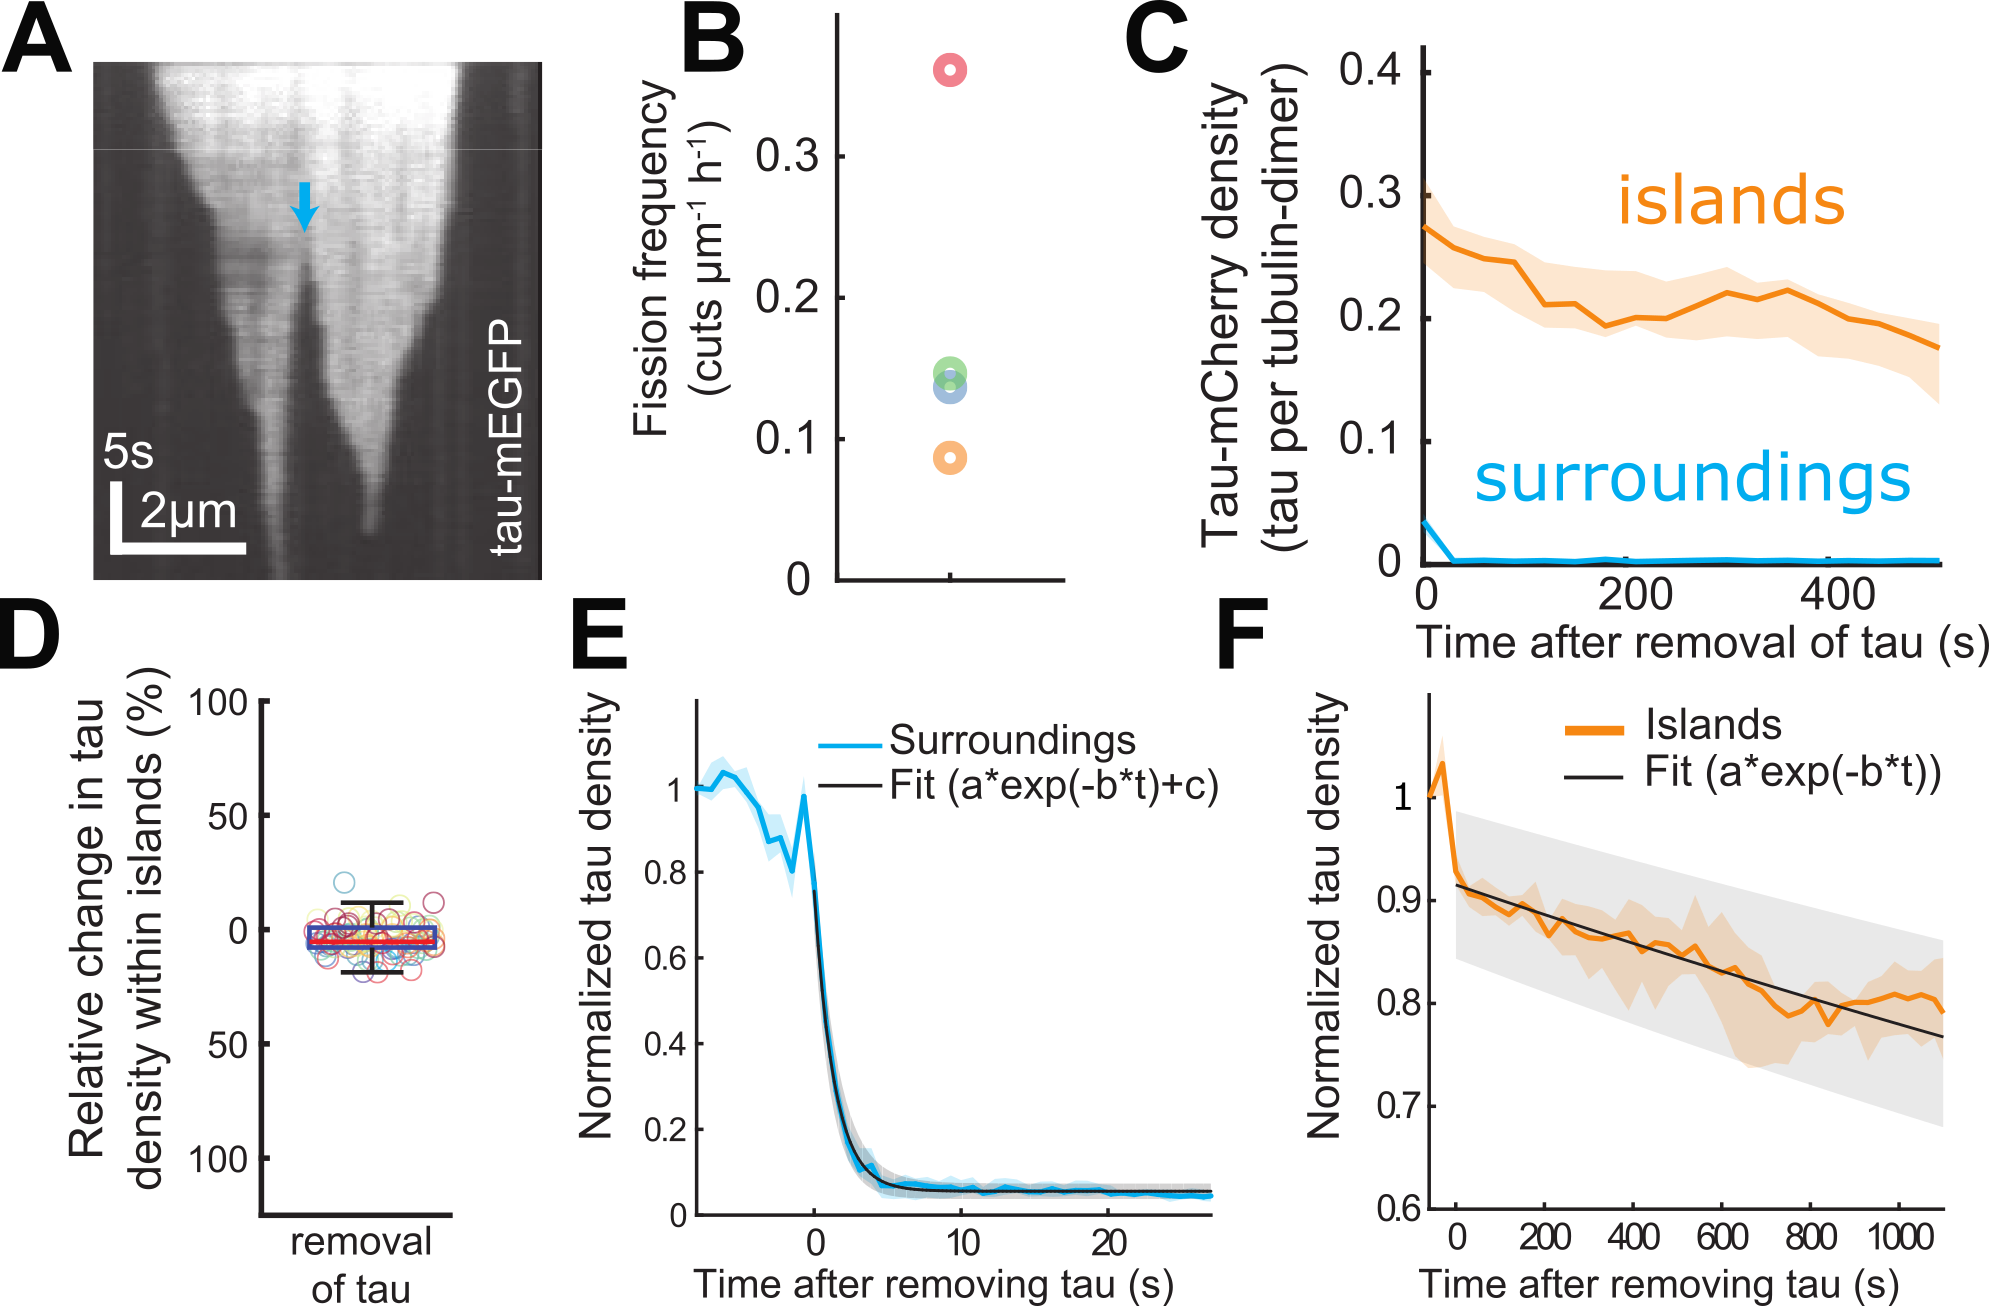
\includegraphics[width=1\linewidth]{Figures/tauSHRINK.png}
	\caption[Tau islands disassemble slowly upon the removal of tau from solution.]{
	\textbf{Tau islands disassemble slowly upon the removal of tau from solution.} (A) Kymograph showing the fluorescence signal of tau on the microtubule after the removal of tau from solution. The blue arrow indicates a fission event that here occurred during island disassembly. (B) Frequency of fissions occurring within islands upon removing tau from solution. Colors encode different experiments. (C) Distribution of island disassembly velocities upon removing tau from solution. Colors encode experiments (same as in B), circles represent deassembly traces. (D) Exemplary time-trace of the tau density inside and outside the islands after removing (20nM) tau from solution (n = 9 microtubules). (E,F) Exemplary time-trace of tau density inside and tau density outside the islands after removing (20nM) tau from solution, analogous to the results presented in E (n = 6 microtubules). Single exponential fits are indicated by solid lines. Panels from \cite{Siahaan2019a}. Panel A is also shown in \cite{Siahaan}.
		}\label{tauSHRINK}
\end{wrapfigure}
These islands, after nucleating from diffraction-limited spots, grew along along a given microtubule to cover more and more of its length \pref{tauGROW}{C,D}. After 75 minutes, most of the microtubule length in a given field of view was covered with islands, with islands still continuing to grow \pref{tauGROW}{E}. When repeating this experiment with higher tau concentrations of 40 and 90nM, microtubules were covered more quickly \pref{tauGROW}{F}, due to a higher nucleation rate of islands \pref{tauGROW}{G} as well as due to faster and more consistent growth at island boundaries \pref{tauGROW}{H}. \par

Generally, the islands did not grow monotonously at their boundaries, but with variable velocities in the order of 25 nm/s, corresponding to about 10 molecules added per second \pref{tauGROW}{H}. Importantly, the tau density in the islands stayed constant during the period of growth \pref{tauGROW}{I}, suggesting that the islands grow by the addition of tau molecules at their boundaries, reminiscent of epitaxial growth of thin films. As another indication that islands are formed by a well-defined tau layer occupying the entire accessible surface of the microtubule, we never observed an increase in the tau density when the boundaries of neighboring growing islands came into contact \pref{tauGROW}{C}.\par

When tau was removed from solution, the islands disassembled slowly from their boundaries, occassionally fissioning inside \pref{tauSHRINK}{A-B}. In contrast to island growth, this island shrinkage rarely halted \pref{tauSHRINK}{B}, and proceeded with a median velocity of approximately 2 tau molecules unbinding per second at a given island boundary \pref{tauSHRINK}{C}. Importantly, the tau density within islands only declined very slowly after removing tau from solution compared to the decline in tau density on all regions outside of islands (the “island surroundings”) \pref{tauSHRINK}{D}. Indeed, while in the surroundings tau unbound with a time constant of about 2 seconds as inferred from the decay of the fluorescence signal \pref{tauSHRINK}{E}, within the islands tau molecules unbound on the timescale of tens of minutes \pref{tauSHRINK}{F}. This extremely low unbinding rate explains the preservation of the islands in absence of tau in solution and suggests that the occasional island fissions observed during disassembly occur after rare events of tau molecules unbinding from inside the island. The large difference in the tau unbinding rates within islands compared to island surroundings, together with the assembly and disassembly kinetics at the island boundaries, indicate that tau molecules in the islands bind to microtubules cooperatively. 

\begin{figure}[h]
\centering
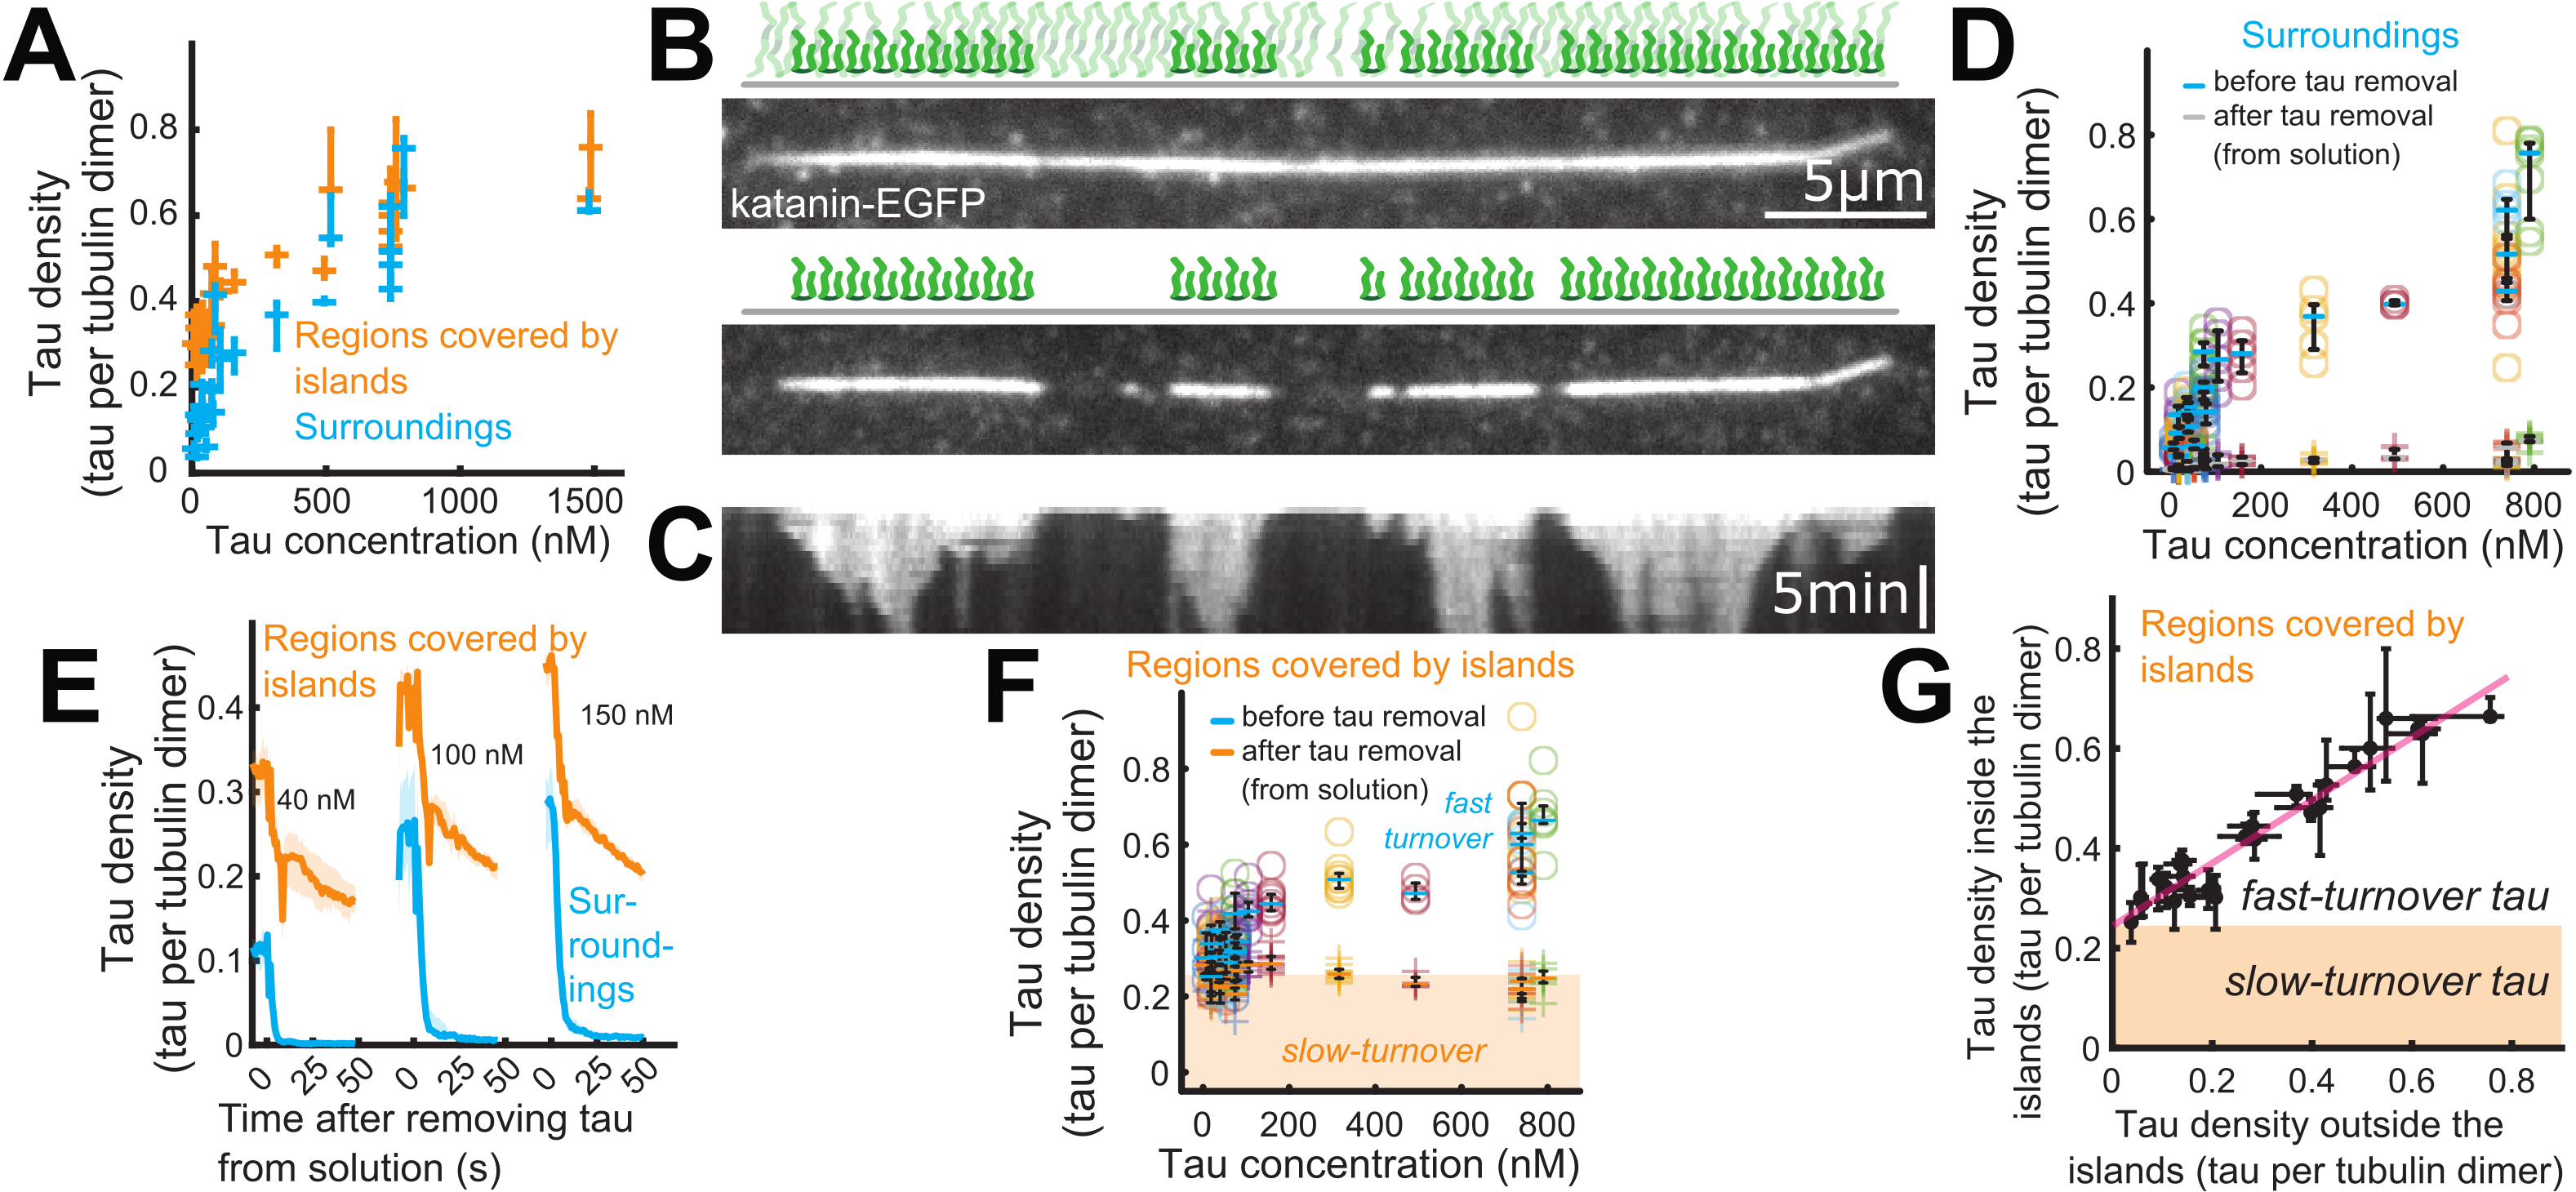
\includegraphics[width=1\linewidth]{Figures/tau_flushouts.png}
\caption[Tau islands are distinguished by cooperative tau binding.]{
\textbf{Tau islands are distinguished by cooperative tau binding} (A) The (equilibrium) density of tau on microtubules plotted against concentration of tau in solution. Horizontal lines indicate the three quartiles. (B) Fluorescence micrographs showing the coverage of a microtubule by tau. Upper panel: 5 minutes after the addition of 0.8 µM tau. Lower panel: 30 seconds after the removal of tau from solution. (C) Kymograph of the experiment presented in B showing the disassembly of the islands after removing tau from solution. (D) Tau densities in microtubule regions surrounding islands, before and after removing tau from solution. (E) Exemplary time-traces of tau density outside and inside the islands during subsequent cycles of adding increasing concentrations of tau followed by removing tau from solution. Experiment such as presented in D and F. (F) Tau densities in microtubule regions with islands, before and after removing tau from solution. (G) The (equilibrium) density of tau on microtubules inside island regions plotted against the density of tau in the surroundings, using the data presented in A. The red line visualizes a linear fit. Points are color-coded by experiment, horizontal lines indicate the three quartiles of each experiment (in some panels the median is indicated by circle). In C and G, the characteristic island density (Main text, Methods) is indicated by the height of the shaded area. Panels from \cite{Siahaan2019a}.
	}\label{tauflushouts}
\end{figure}

To more thoroughly explore whether and how the phenomena we observed were concentration-dependent, we conducted additional experiments, increasing the range of tested tau concentrations. Our observations revealed that island formation did not occur below a critical tau concentration of approximately 5 nM (n = 245 microtubules in 5 experiments; these experiments were performed by my colleague Valerie Siahaan). Above this threshold, we noted that the tau density both within and outside the islands increased with the tau concentration in solution \pref{tauflushouts}{A}. We had noticed this previously already with our experiments at 20, 40 and 90nM tau, yet with much larger concentrations it in addition became apparent that tau binding to microtubules in our buffer condition reaches a saturation point at around 1000nM \pref{tauflushouts}{A}. Moreover,under such saturated binding conditions, the density on the microtubule appears to be uniform \pref{tauflushouts}{A}, i.e., a distinction between islands and surroundings based on tau density can no longer be made. However, upon removing tau from solution, in areas surrounding the islands, the tau density rapidly returned to background levels within seconds \pref{tauflushouts}{B-E}, consistent with our previous surrounding-related findings when removing 20nM Ase1 \pref{tauSHRINK}{E}. Meanwhile, the islands persisted \pref{tauflushouts}{B-C} as observed previously \pref{tauSHRINK}{A}. However, at higher Ase1 concentrations it became apparent that the tau density within the islands exhibits a two-phase decay upon removal of tau: an initial rapid, uniform decrease along the entire island length, followed by a slower density reduction \pref{tauflushouts}{E}. Importantly, the tau density within the islands, following the rapid density drop, consistently measured 0.26 ± 0.05 tau molecules per tubulin dimer (average ± SD, n = 101 microtubules, 14 experiments, Methods). This value remained constant regardless of the initial tau concentration in solution \pref{tauflushouts}{F}. \par

Combining these results with our findings from \aref{tauGROW}{} and \aref{tauSHRINK}{}, we conclude that cohesive islands on microtubules form through the cooperative binding of tau molecules, resulting in their slow unbinding. At physiological tau concentrations \parencite{Wegmann}, ranging from 0.5 to 1.5 µM, we observed the co-localization of rapidly turning over tau molecules with the islands. The density of these co-localized tau molecules, which appears to correlate with the tau concentration in solution similarly to the tau density outside the islands \pref{tauflushouts}{G}, does not seem to be part of the cooperative island formation process. \par

\begin{figure}[h!]
	\centering
	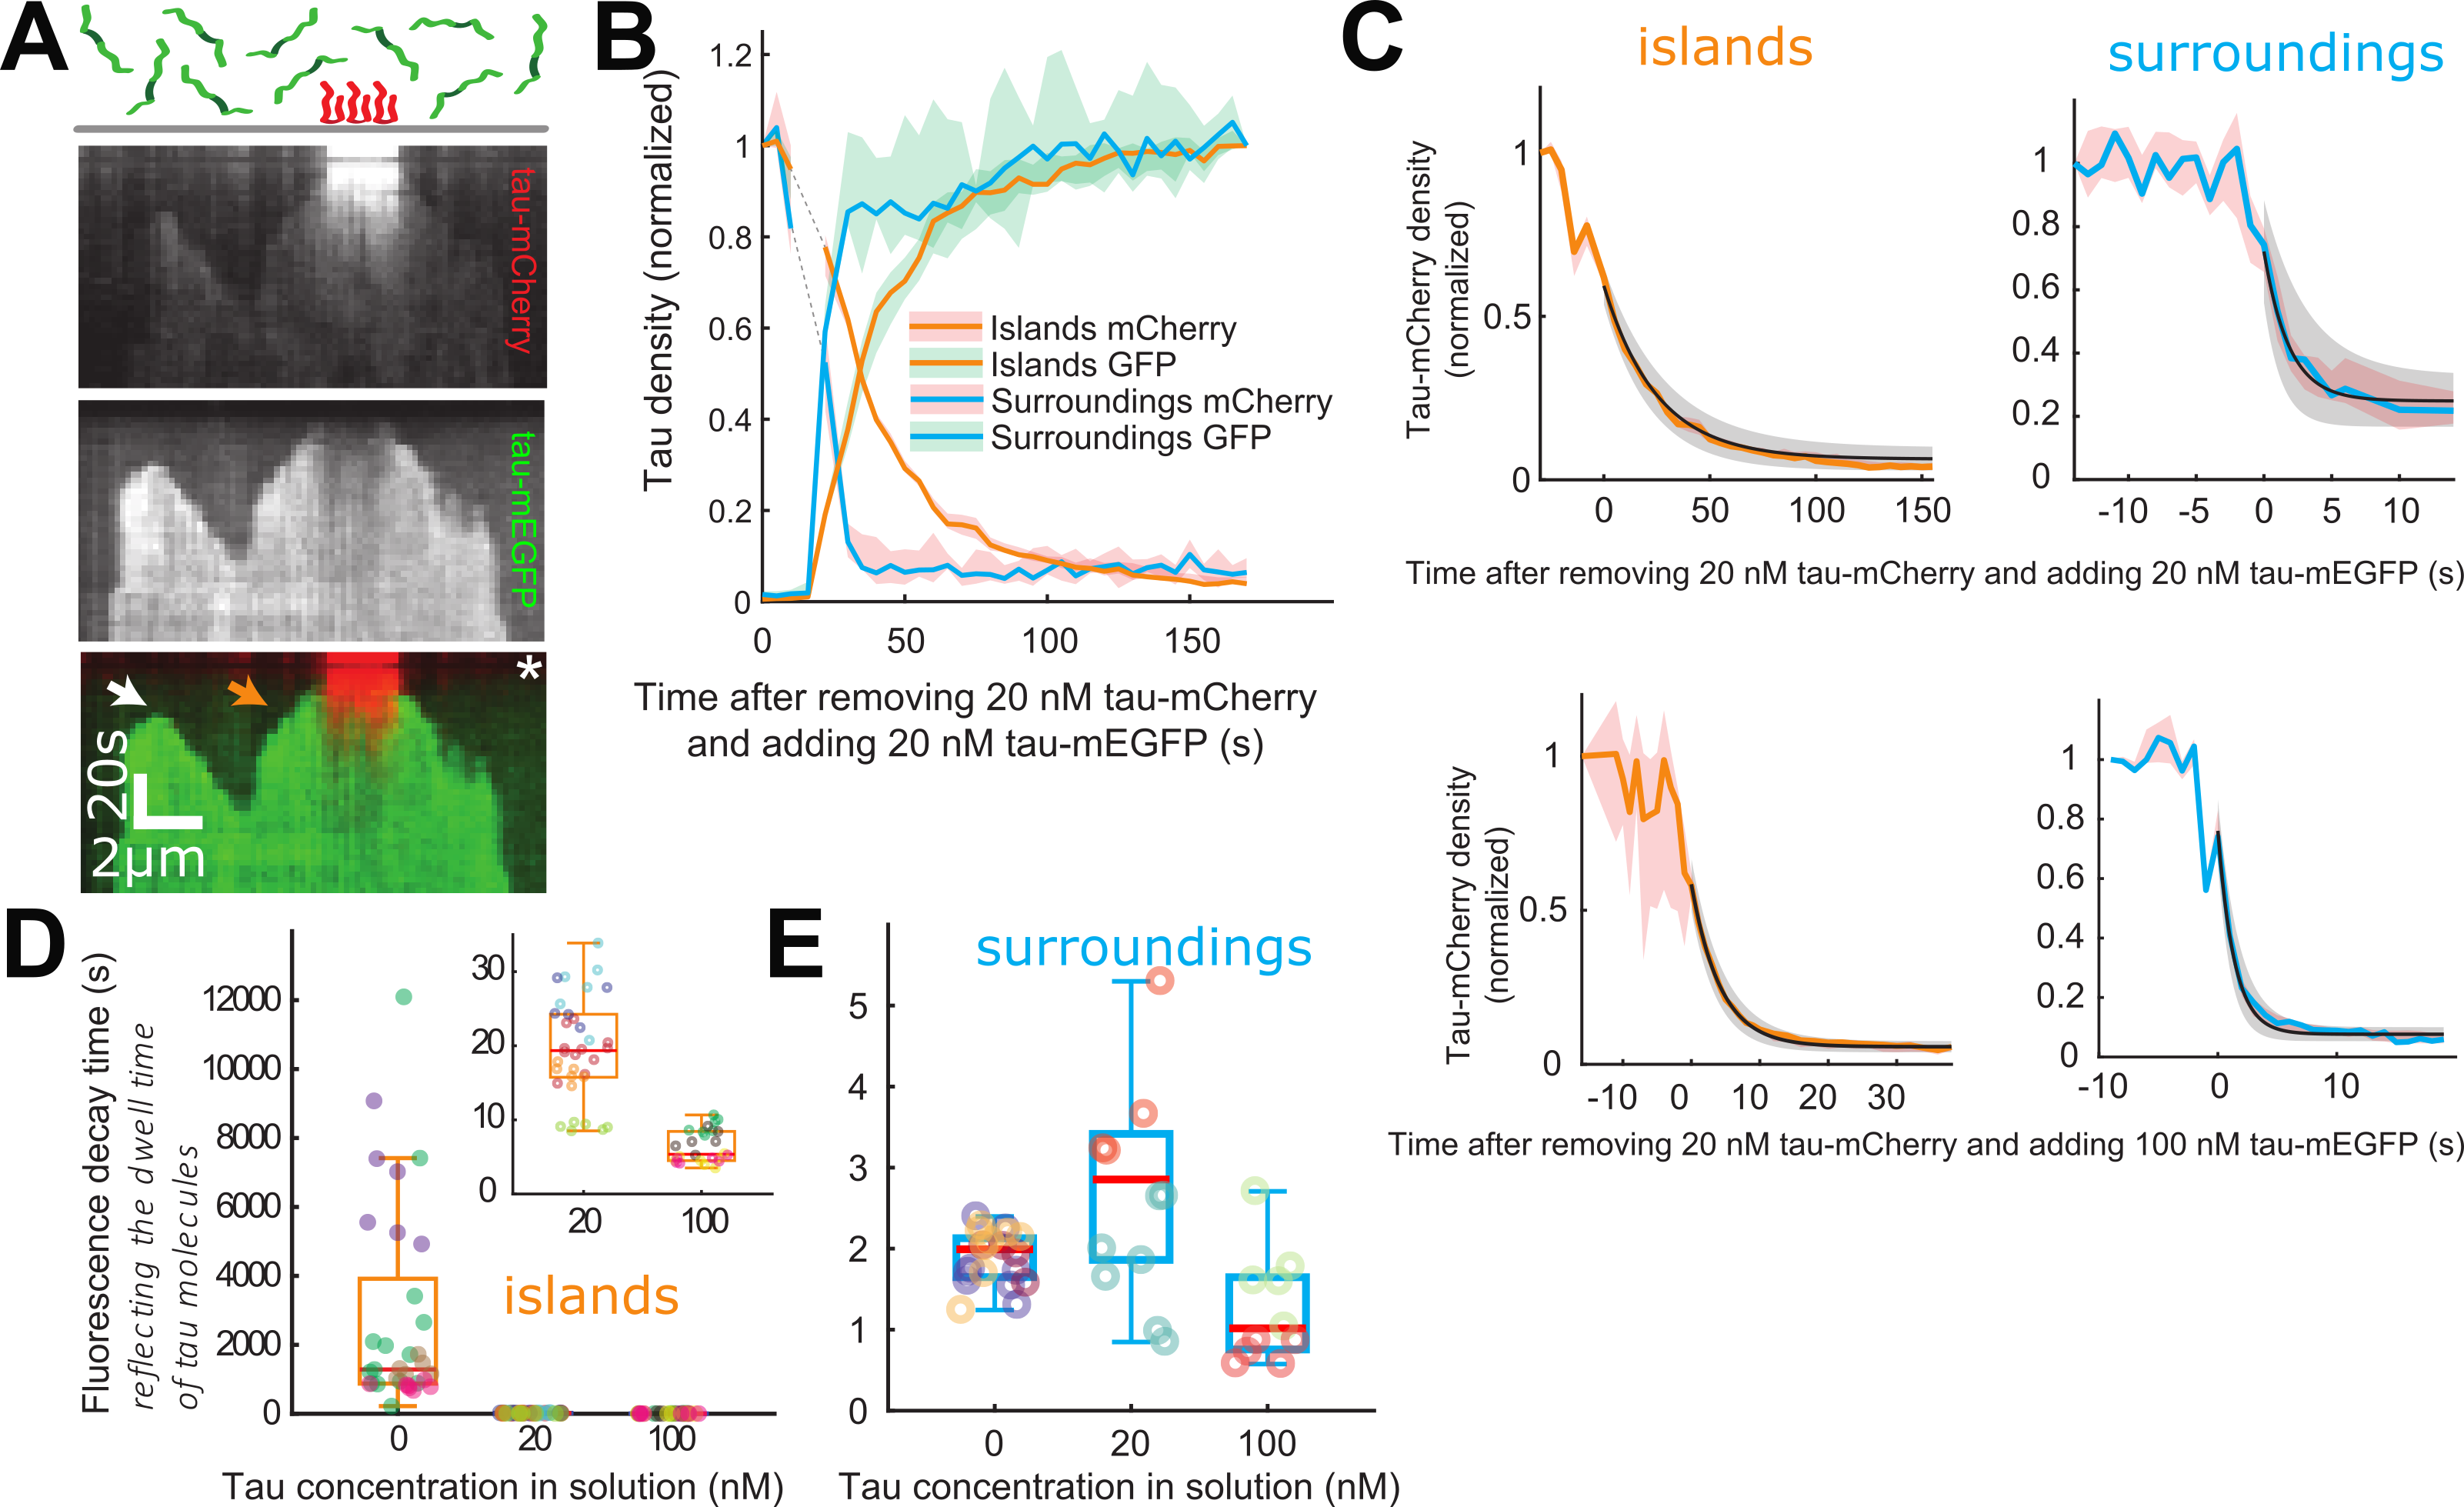
\includegraphics[width=1\linewidth]{Figures/tau_EXCHANGE.png}
	\caption[Tau molecules in the islands exchange with tau in solution.]{
	\textbf{Tau molecules in the islands exchange with tau in solution.} (A) Multichannel kymograph showing an island pre-formed in presence of 20 nM tau-mCherry (red). After the addition (time marked by white asterisk) of 20 nM tau-mEGFP (green), removing most of the tau-mCherry from solution, tau-mEGFP replaces tau-mCherry inside and outside of the islands. An example of an island resuming its growth by the addition of tau-mEGFP is marked by an orange arrow, a nucleation event is marked by a white arrow. (B) Exemplary time-trace of normalized tau-mCherry and tau-mEGFP density inside and outside the islands after exchange of 20 nM tau-mCherry for 20 nM tau-mEGFP. Photo-bleaching during this experiment was negligible (Methods); the dotted line indicates that the sample was out of focus at the time. (D) Dwell times of tau-mCherry derived from fitting exponential decay functions to tau densities over time in the surroundings of islands. (E) Same representation as D, for island regions. The inset displays the 20 nM and 100 nM boxes on a magnified y-scale. Data points are color-coded by experiments. Panels from \cite{Siahaan2019a}. Panels A and E are also shown in \cite{Siahaan}.
		}\label{tauexchange}
\end{figure}

To further explore the dynamics of tau molecules in the islands, we formed islands using 20 nM tau-mCherry and, after 15 minutes, replaced the assay buffer by a solution containing 20 nM tau-mEGFP. Outside the islands, tau-mCherry was replaced quickly by tau-mEGFP \pref{tauexchange}{A}. This included the growth of new islands, which now proceeded by addition of tau-mEGFP \pref{tauexchange}{A}. However, within the islands, tau-mCherry visibly remained bound to microtubules for longer \pref{tauexchange}{A,B}. We quantified this effect by fitting the tau density in a given region at different time points to an exponential decay function \pref{tauexchange}{C}: In the low-density regions, surrounding the islands, tau-mCherry dissociated from the microtubules with an average residence time of about 3 seconds \pref{tauexchange}{D}, a value comparable to the residence time where tau was completely removed from solution without replacement \pref{tauSHRINK}{E}. By contrast, within the islands tau-mCherry dissociated markedly slower, with an average residence time of 20 ± 7 s (average ± SD) seconds \pref{tauexchange}{E}. This value is, however, substantially faster than in the situation when tau was completely removed from solution, in which case the dwell time was 45 ± 46 min (compare to \aref{tauSHRINK}{F}). Thus, we observed that tau unbinding from the islands depends on the tau concentration in solution. As another piece of evidence confirming this dependence, we observed that tau-mCherry unbound form islands even faster when adding 100nM tau-mEGFP as compared to the addition of 20nM tau-mEGFP (in this case, the dwell time was 6.4 ± 2.1 s) \pref{tauexchange}{E}.\par

To further study the spatio-temporal interaction dynamics of tau and microtubules, we formed islands using a mixture of 20 nM tau-mCherry and 1 nM tau-mEGFP. This strategy allowed us to observe the motion of individual tau-mEGFP molecules even within tau islands, 

\begin{wrapfigure}{l}{0.5\textwidth}
	\centering
	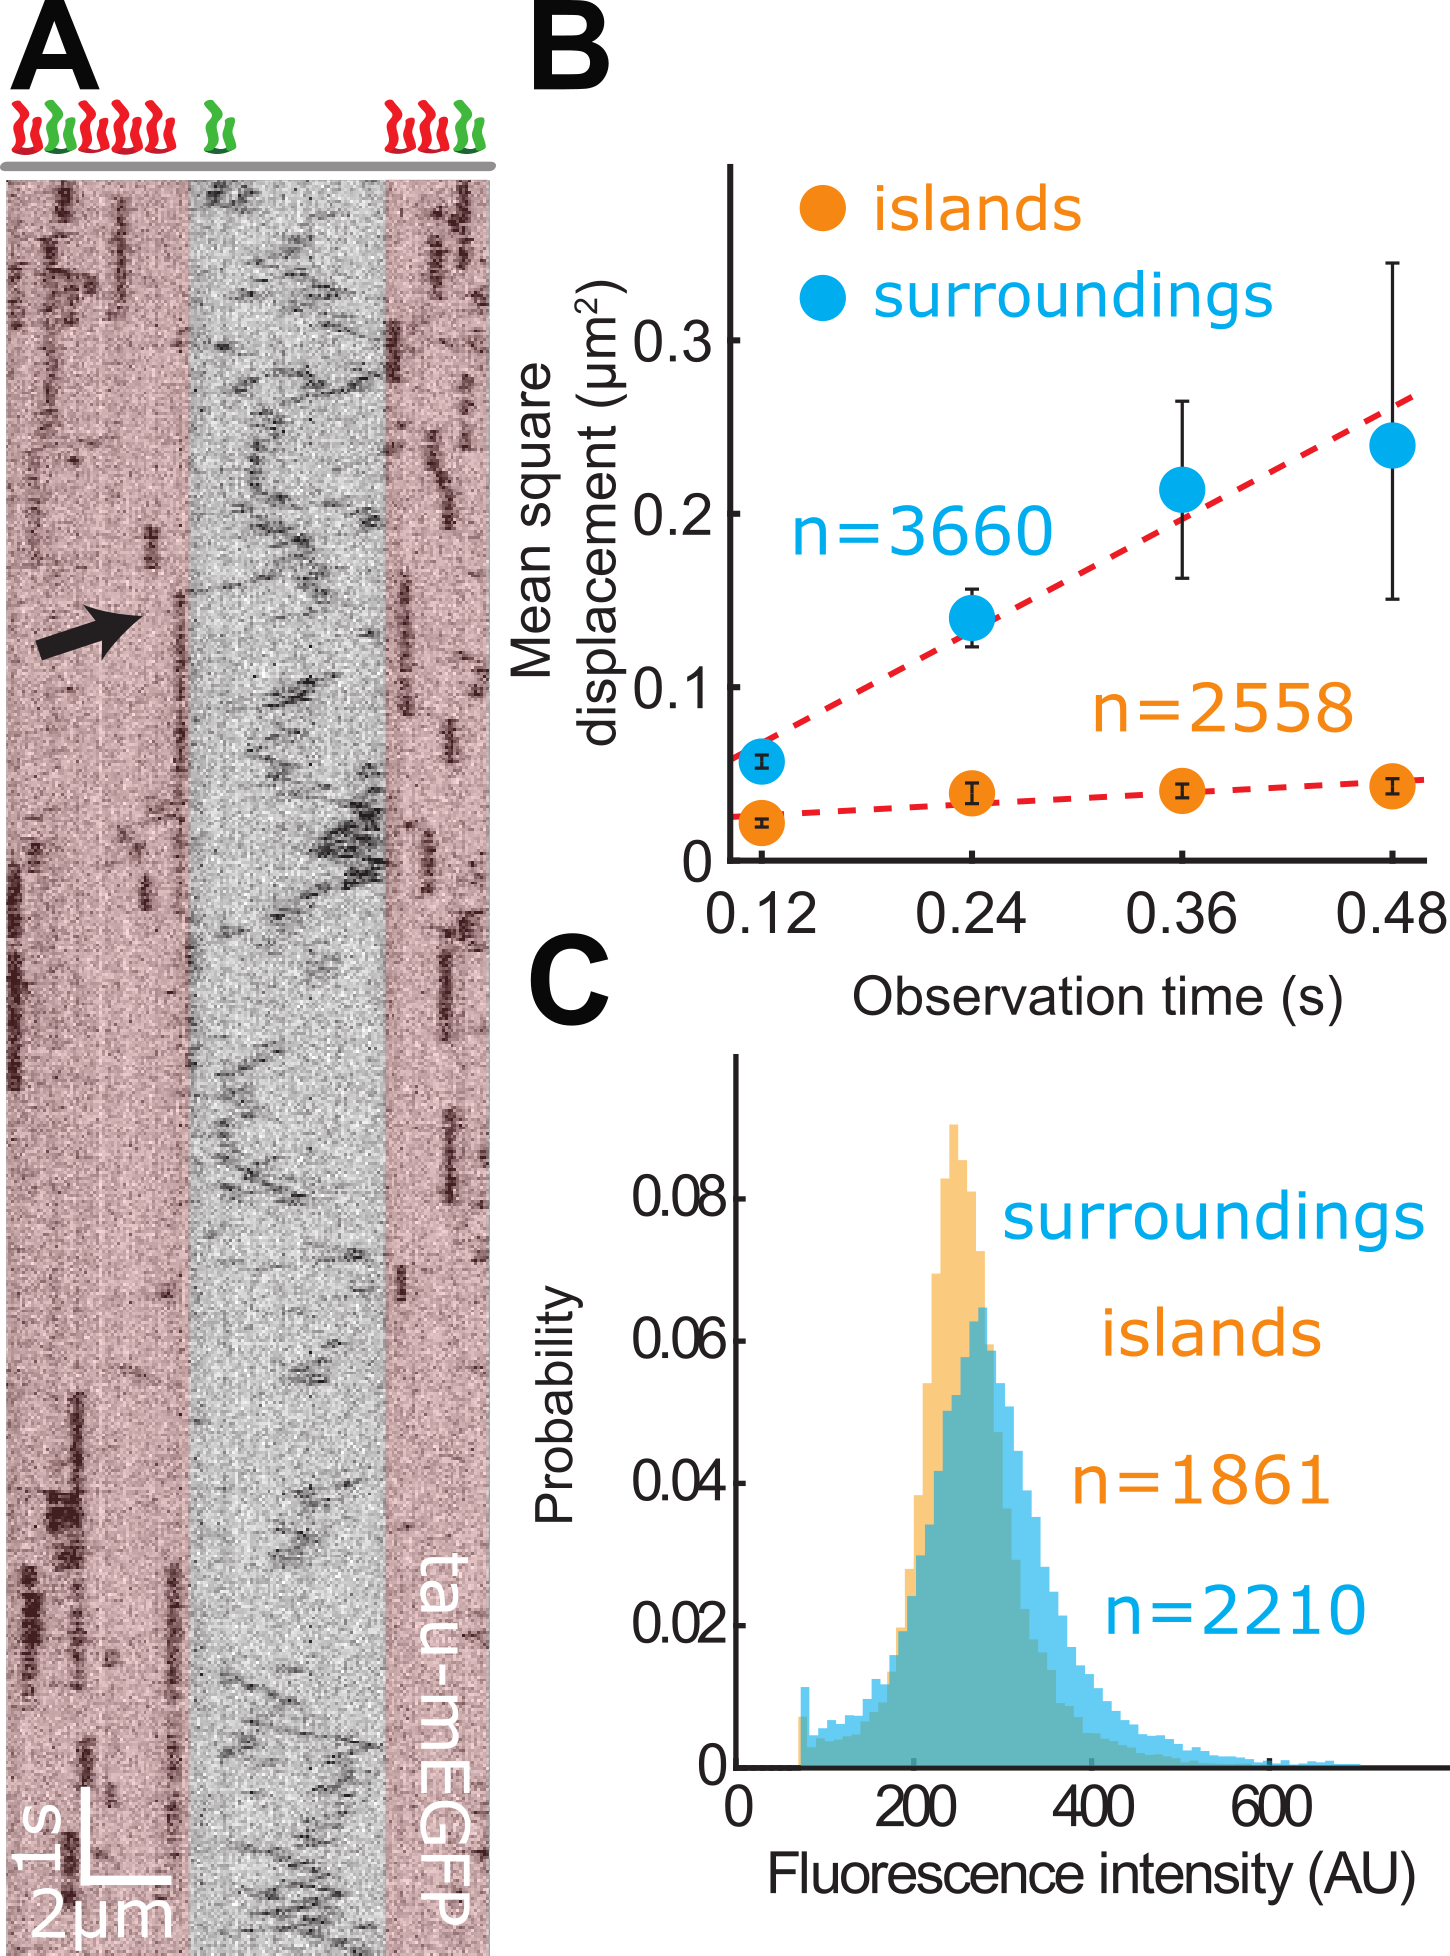
\includegraphics[width=1\linewidth]{Figures/tau_singleMolecules.png}
	\caption[Tau molecules are stationary within the islands.]{
	\textbf{Tau molecules are stationary within the islands.} (A) Intensity-inverted kymograph showing single tau-mEGFP molecules interacting with a microtubule covered by two tau-mCherry islands (light red regions) at 20nM tau-mCherry in solution. Black arrow: An event where a diffusing tau-mEGFP molecule gets associated with an island. (B) Mean square displacement over time of single tau-EGFP molecules inside and outside tau-mCherry islands. (C) Histograms of fluorescence intensities of single tau-mEGFP particles bound to microtubules in experiments as presented in A. (D) Same as A, however, with 100nM tau-mCherry in solution instead of 20nM. Orange arrow: A brief and diffusive interaction of a tau molecules inside the island. Blue arrows: Island-bound tau molecules switche to a (more) diffusive binding mode. White arrow: A brief tau interaction within islands. Panels from \cite{Siahaan2019a}, except for panel D, which is published only in this thesis (experiment conducted by Valerie Siahaan, data analyzed and interpreted by me). Panel A is also shown in \cite{Siahaan}.
		}\label{tausingle}
\end{wrapfigure}
\noindent as these islands were mainly comprised of tau-mCherry molecules. In the low-density regions, single tau-mEGFP molecules diffused rapidly \pref{tausingle}{A}. By contrast, in the islands the tau-mEGFP molecules did not display any noticable movement \pref{tausingle}{A}. Quantifying these phenomena (Methods), we measured that outside the islands, tau molecules diffused with a diffusion constant of 0.27 ± 0.15 $\mu m^2s^{-1}$ (95\% confidence bounds) \pref{tausingle}{B}, comparable to values reported before by \cite{Hinrichs2012b}. Within the islands, we measured tau-mEGFP molecules to have a diffusion constant of 0.027 ± 0.016 $\mu m^2s^{-1}$ \pref{tausingle}{B}. To test whether we indeed observed single tau molecules rather than conglomerates which had formed in solution, we generated fluorescence intensity histogram of individual tau-mEGFP particles \pref{tausingle}{C}. These exhibited a single Gaussian profile in the islands just as in their surroundings, indicating that tau-tau interactions indeed occurred only on the microtubule lattice. We also formed islands using a mixture of 100 nM tau-mCherry and 1 nM tau-mEGFP. Consistent with the results shown in \aref{tauflushouts}{}, we observed diffusive and/or brief interactions of tau molecules inside islands \pref{tausingle}{D}. It also beas noting that occasionally, single tau-mEGFP molecules initially diffusing outside an island became stationary when associating with an island boundary \pref{tausingle}{A}, hinting at growth of the islands from the boundary.\par

\begin{figure}[h!]
	\centering
	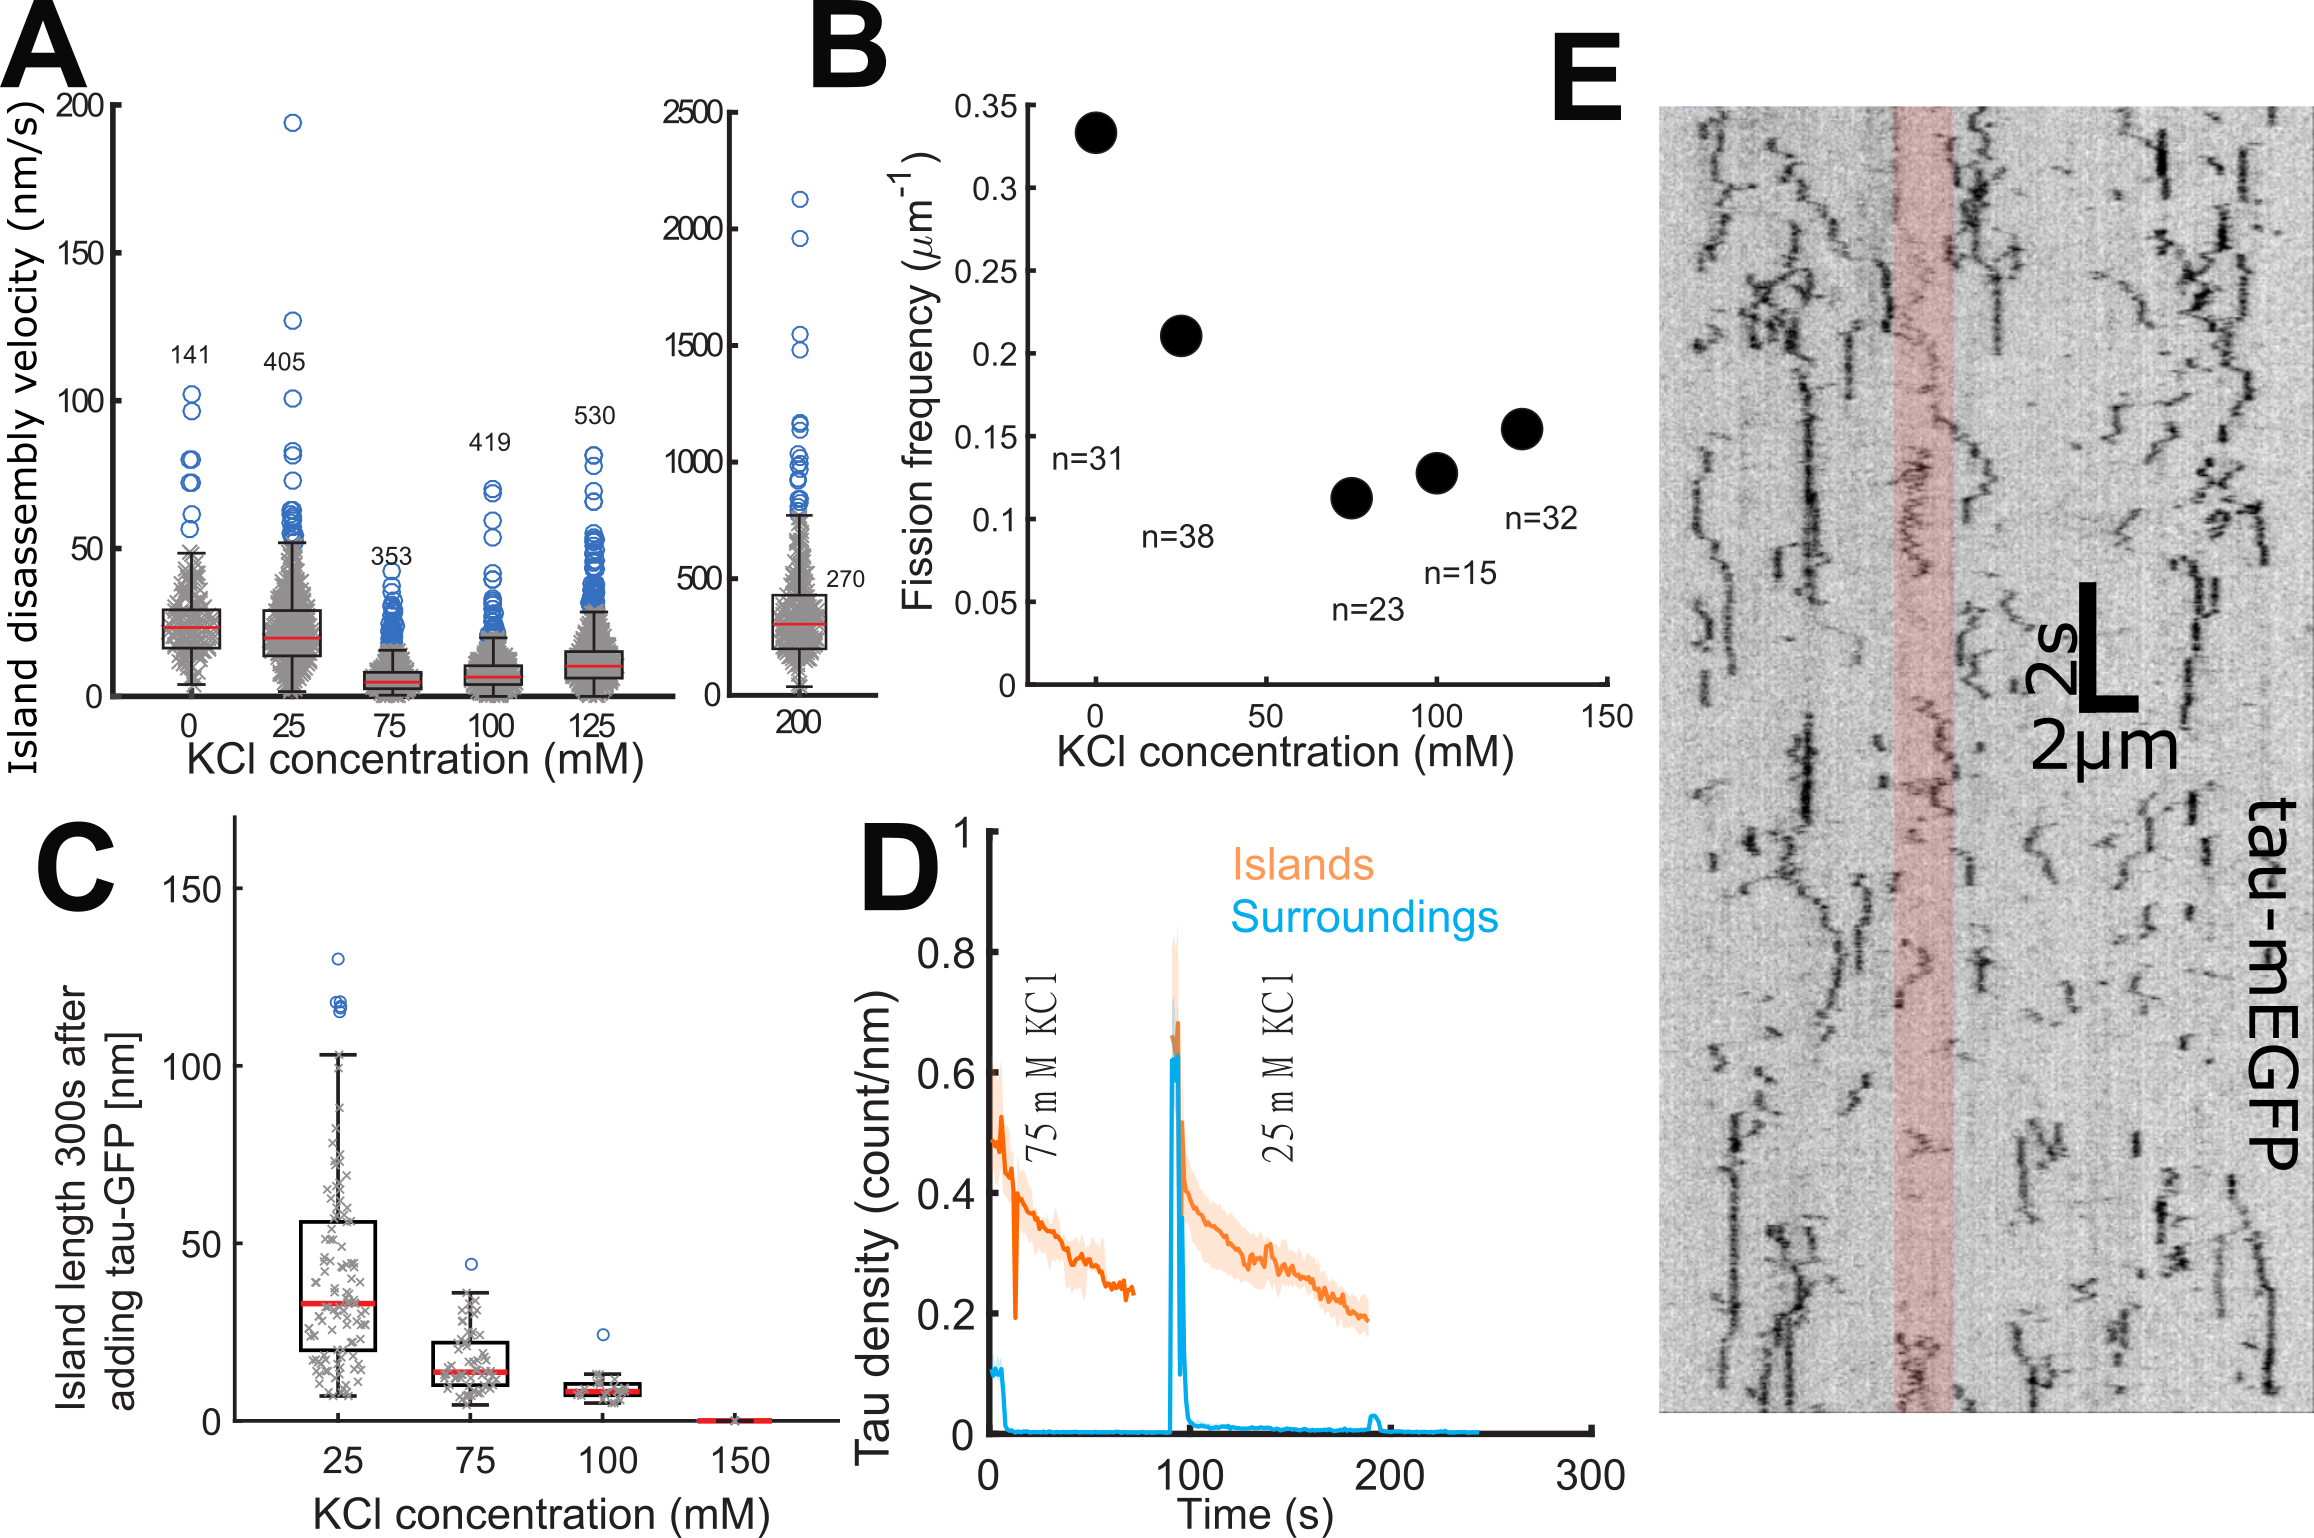
\includegraphics[width=1\linewidth]{Figures/tausalt.png}
	\caption[The preferred binding mode of tau varies with ionic strength.]{
	\textbf{The preferred binding mode of tau varies with ionic strength.} (A,B) Island disassembly velocities and fission frequencies at different concentrations of KCl (after tau had been removed from solution; islands had been grown at 75mM KCl). Numbers show the number of measured disassembly periods (panel A) or observed fissions (panel B). (C) Lengths of islands measured 300s after adding 40nM tau at varying concentrations of KCl. (D) Cycles of adding and removing 100nM tau to/from solution (additions at t=-100s and t=100s, removals roughly at t=10s and t=110s). In the second cycle, the solution contained only 25mM KCl rather than 75mM, which was used in all previously shown experiments. Bleaching was not negligible in this experiment. (E) Intensity-inverted kymograph showing single tau-mEGFP molecules interacting with a microtubule covered by a tau-mCherry island (highlighted by the red area) at 25mM KCl. Findings shown in this figure have not been published yet.
		}\label{tausalt}
\end{figure}

Finally, we were interested in exploring some plausible determinants of island assembly beside tau concentration. First, because the N-terminus of tau mediates tau-tau interactions \parencite{Gamblin2003}, we attempted to grow tau islands with a truncated tau construct comprising the four-repeat microtubule-binding domain and the C-terminus but lacking the N-terminus (tau$\Delta$N-mEGFP, \aref{tauconstructs}{}). Although tau$\Delta$N-mEGFP did interact with the microtubules, we did not observe any island formation even at 0.5 µM tau$\Delta$N-mEGFP (these experiments were performed by my colleague Valerie Siahaan). Second, we varied the ionic strength of our buffer solution by varying the concentration of KCl (these experiments were largely performed by me; for reasons of space we did not include these findings in \cite{Siahaan2019a}). We noticed that increasing as well as decreasing the concentration of KCl from the level we had used for the experiments we have reported on so far, namely 75mM, both tended to decrease the stability of tau islands: 0, 25, 100, and 125nM KCl islands disassembled quicker once tau was removed from solution than at 75mM KCl \pref{tausalt}{A,B}. Disassembly speed was drastically higher at 200mM KCl \pref{tausalt}{A right panel}. Generally, tau binding to the microtubule was less pronounced at higher KCl concentrations, both in terms of island formation and binding to surrounding regions (data not shown). However, interestingly, at 0 and 25mM KCl, island assembly was more pronounced than at 75mM KCl \pref{tausalt}{C}. At the same time, at these low KCl concentrations, more tau bound to the microtubule via the diffusive binding mode, visible from the high tau densities in the surrounding regions \pref{tausalt}{D}. Consistent with the observation that islands at lower ionic strengths were less stable, when looking at single tau-mEGFP molecules in a tau-mCherry-dominated environment, we observed that the distinction between binding within the islands versus binding outside the islands was less clear-cut than at 75mM KCl \pref{tausalt}{E}. Tau molecules appeared to switch regularly between diffusive and stationary interactions within islands, though the diffusive interactions appeared more tightly bound to the microtubule than outside the islands \pref{tausalt}{E}. We had observed such switches already at 75mM KCl, though at that condition these switches were much less prevalent \pref{tausingle}{D}.\par

Combined, our results show that tau molecules bind to microtubules in two distinct binding modes. The diffusive binding mode had already been described before \parencite{Hinrichs2012b}. However, we together with \cite{tan2019microtubules} discovered another, cooperative, binding mode, which results in the formation of what we termed tau islands (in more recent publications on the topic the term "envelopes" is used, see e.g. \cite{siahaan2022microtubule}). This cooperative binding mode, unlike the diffusive mode, is dependent on the N-terminus region of tau. The strength of this cooperative binding mode moreover varies differently with ionic strength than the strength of the diffusive binding mode.
	\section{Interaction Patterns Between Ase1 and Dynamic Microtubules}
\label{sec:Ase1}

\subsection{The effect of Ase1 on microtubule dynamic instability}
\begin{figure}[h]
    \centering
    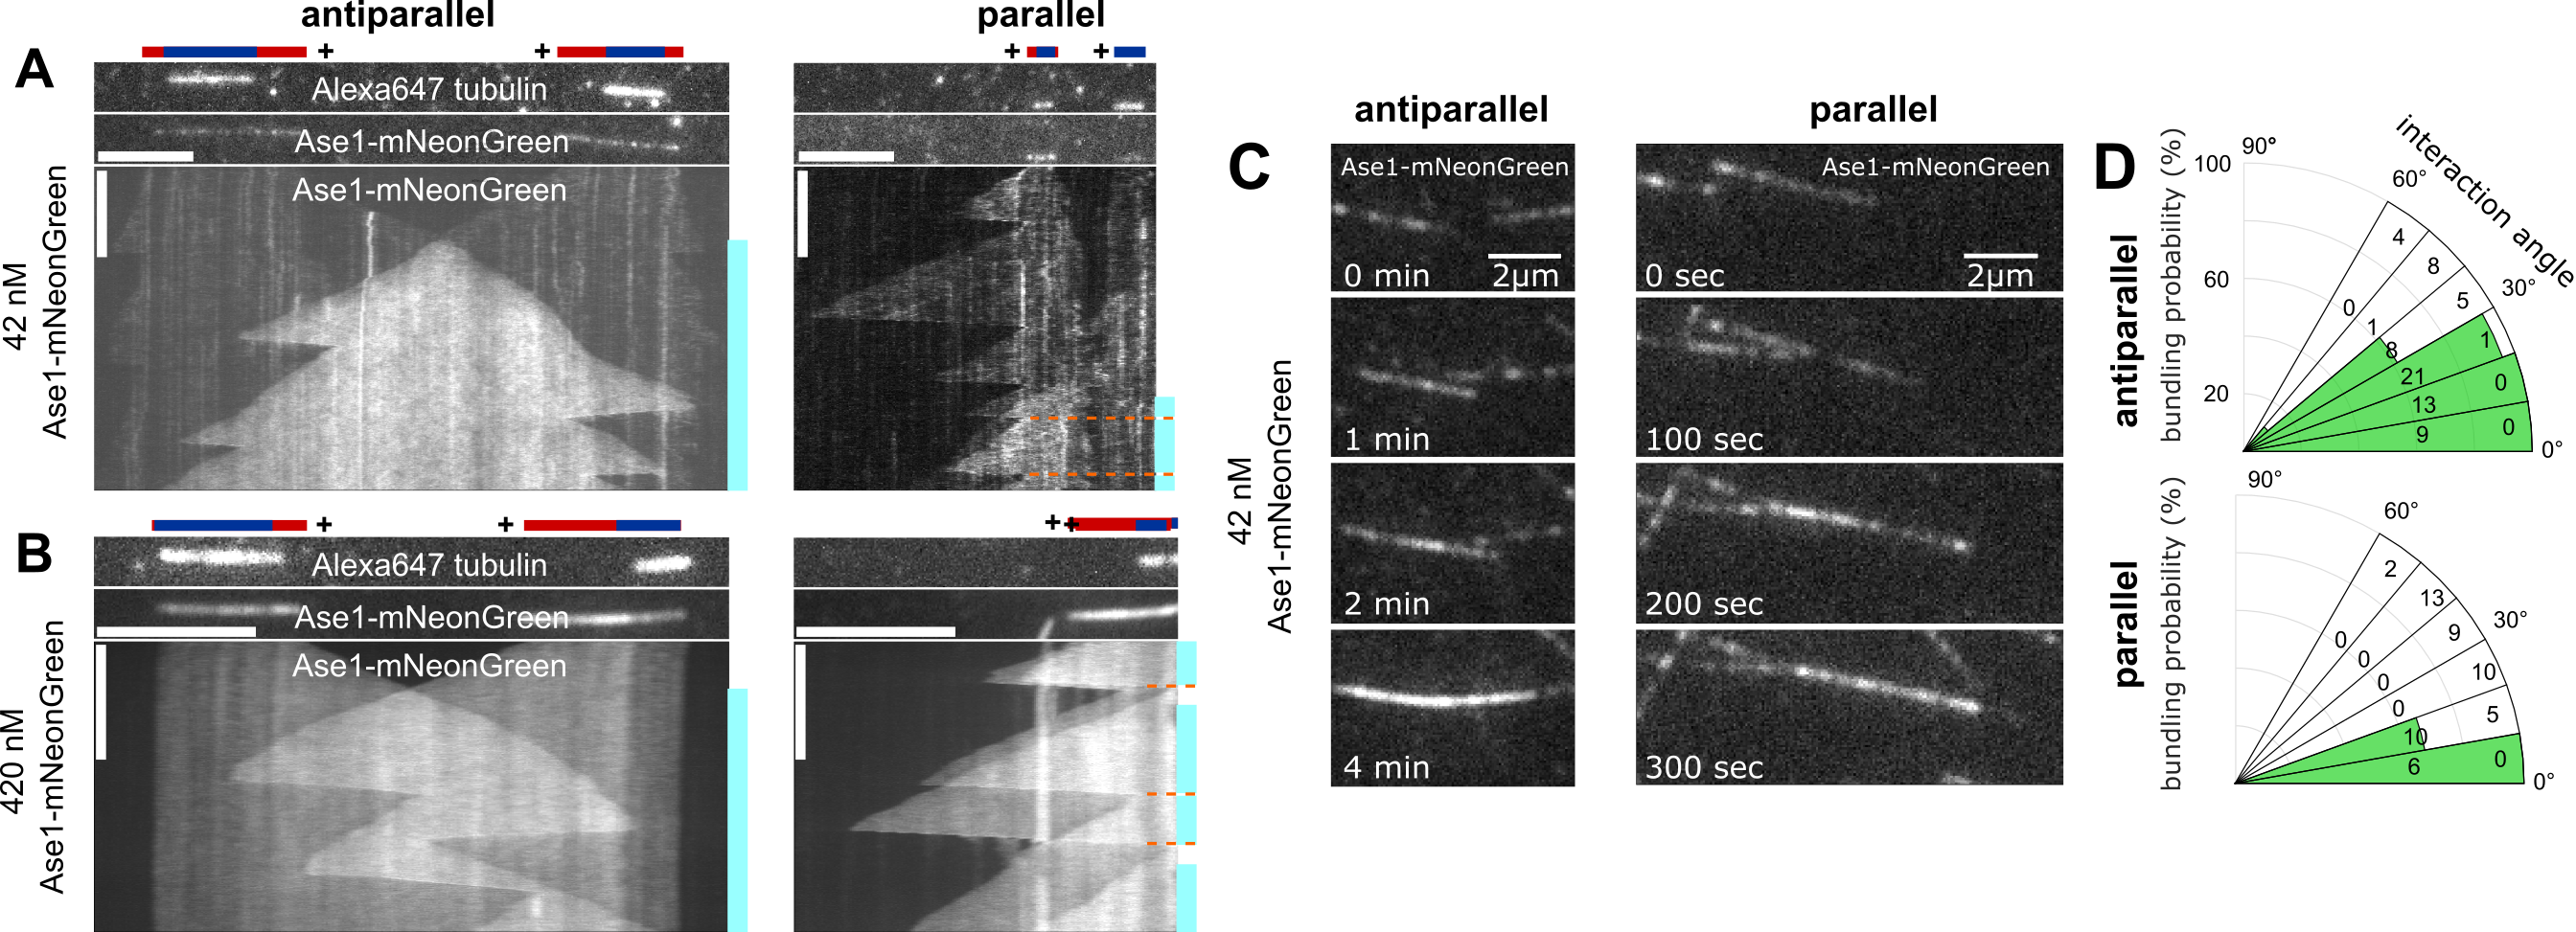
\includegraphics[width=1\linewidth]{Figures/ase1_1a.png}
    \caption[With dynamic microtubule extensions and Ase1, we observed microtubule bundling as previously reported.]{
    (A) Kymographs of an antiparallel (left panel) and a parallel microtubule overlap forming due to the microtubules polymerizing such to enable bundling by Ase1, which is present in solution (42nM). The scale bars are 5 micron and 10 minutes. In sketches, dynamic extensions with GDP lattices are red, and stabilized GMPCPP seeds are blue. The teal bars next to kymographs indicate the presence of regions of overlap (we only counted regions where the two partaking microtubule regions are constituted by GDP-tubulin, i.e., a seed stabilized by GMPCPP did not count). The orange lines indicate a termination of the overlapping period, as evaluated for \autoref{ase1b}A. (B) Same representation as A showing events from experiments performed at 420nM Ase1. (C) Snapshots of different events than shown in A and B, illustrating microtubule bundling (at 42nM). (D) Bundling probability for situations when microtubule plus ends encountered other microtubules, in either parallel or antiparallel orientation, versus the initial angle of interaction (results pooled for all Ase1-mNeonGreen concentrations). The outer numbers denote the numbers of recorded crossings at the respective angle, while the inner numbers denote the numbers of bundling events (the sum of both numbers is the total number of observed events). Panels taken from \cite{Krattenmacher2024}.
        }\label{ase1a}
\end{figure}
To investigate the interaction dynamics between diffusible microtubule crosslinkers and microtubules, we employed total internal reflection fluorescence (TIRF) and interference reflection microscopy (IRM) (\autoref{sec:microscopy}) time-lapse imaging of immobilized, GMPCPP-stabilized microtubule seeds in the presence of 30 µM free tubulin and varying concentrations of Ase1 (\autoref{methods}). At concentrations of 42 nM and 420 nM Ase1, we observed dynamic, Ase1-decorated microtubule extensions polymerizing from the microtubule seeds \pref{ase1a}{A,B}. When two microtubule plus ends, emanating from different seeds and polymerizing towards each other, encountered each other, the microtubules either bundled or crossed, depending on the angle of incidence. Typically, at high angles, the microtubules crossed and only interacted at the crossing point, while at small angles, either parallel or antiparallel associations could be formed \pref{ase1a}{C}. As previously reported \parencite{Janson2007}, antiparallel bundles formed even at large initial angles of incidence (up to 40°), while parallel bundles only formed at initial angles below 20° \pref{ase1a}{D}.\par
\begin{wrapfigure}{l}{0.4\textwidth}
    \centering
    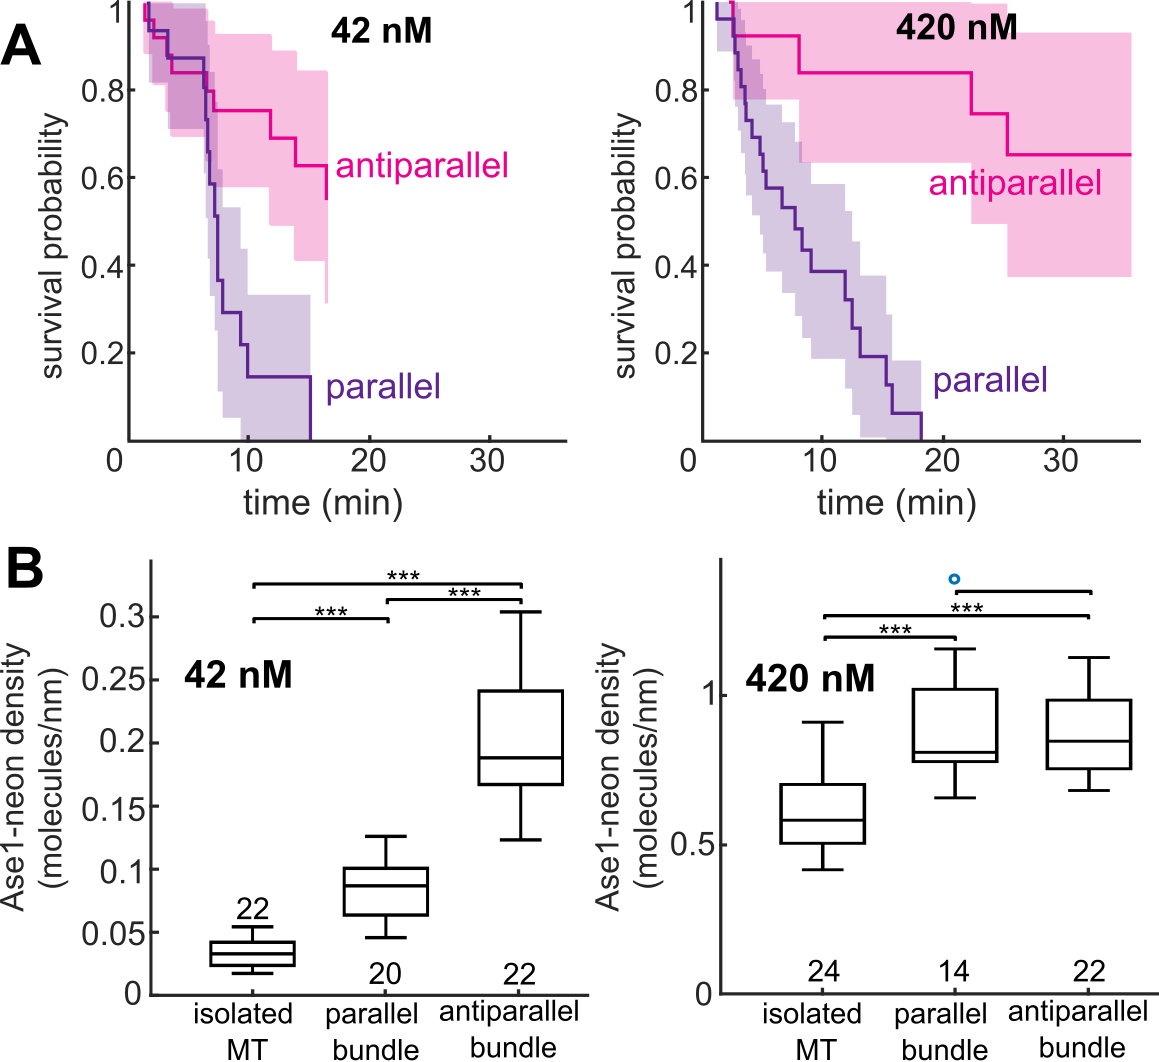
\includegraphics[width=1\linewidth]{Figures/ase1_1b.png}
    \caption[Ase1 selectively stabilizes antiparallel overlaps.]{
    (A) Survival probability of antiparallel and parallel overlaps, showing the probability that an overlap formed by two dynamic MT extensions persists at a given time after its formation (Methods). Semitransparent regions indicate 95\% lower and upper confidence bounds. (B) Quantification of the density of Ase1-mNeonGreen on isolated MTs and (anti)parallel bundles (Methods). The numbers below the boxes denote the number of analyzed microtubule bundles. Panels show data for MT plus ends (minus ends generally were not analyzed). Panels taken from \cite{Krattenmacher2024}.
        }\label{ase1b}
\end{wrapfigure}
Quantitative analysis revealed increased lifetimes of antiparallel overlaps compared to parallel ones\pref{ase1b}{A} Notably, at 42 nM Ase1 in solution, the Ase1 density on antiparallel overlaps was an order of magnitude higher than on parallel ones\pref{ase1b}{B} consistent with the previously reported differential affinities \parencite{Janson2007}. At 420 nM Ase1, we observed the density of Ase1 to be similar on antiparallel and parallel bundles, roughly twice the density found on isolated microtubules\pref{ase1b}{B} This possibly indicated that, at this high concentration, a similar number of Ase1 molecules was present within parallel and antiparallel overlaps. Note, however, that this value represents the total density of Ase1 at the bundle, which might differ from the density of Ase1 molecules directly engaged in MT crosslinking by being bound simultaneously to both microtubules. Despite similar decoration levels by Ase1, antiparallel overlaps were still significantly more stable than parallel ones\pref{ase1b}{A} Given the low polymerization velocity of minus ends, we very rarely observed antiparallel overlaps formed by two minus ends encountering each other, and we thus could not meaningfully quantify the associated lifetime. Generally, we chose to not analyze minus ends given that they are not dynamic \textit{in vivo} \parencite{dammer}.\par

To test whether the relative stability of antiparallel overlaps was caused by Ase1 crosslinking or the bundling itself (as was requested by a reviewer), we also conducted experiments at 10nM Ase1. At this concentration, we observed significantly less Ase1 within antiparallel bundles \pref{ase1c}{A}, and indeed, antiparallel bundles were no more stable than parallel bundles \pref{ase1c}{B}. Also, at 10nM Ase1 we observed antiparallel microtubules to no longer bundle as readily as at higher Ase1 concentrations \pref{ase1c}{C}. While we could detect an Ase1 signal at antiparallel overlaps, we did observe events where Ase1 crosslinking apparently was not strong enough to keep a MT plus end bundled to the MT along which it was growing in an antiparallel orientation \pref{ase1c}{D,E left panel}. Finally, to test whether microtubule bundling in our assays was partially a result of molecular crowding (and not Ase1), we performed an assay at 0nM Ase1. In absence of Ase1, microtubules never bundled, even when very close to each other over extended periods of time, indicating that molecular crowding did not play a role in the microtubule bundling we observed \pref{ase1c}{F}. \par

The relative stability of antiparallel overlaps at high Ase1 concentrations may at least partly owe to the fact that antiparallel overlaps grow with twice the speed of parallel overlaps (since both microtubules polymerize in opposite directions, however it should be noted that once a minus end has been surpassed the antiparallel overlaps does no longer grow as quickly on the side in question); hence, there is more opportunities for rescues to occur during depolymerization. However, our kymographs suggested that antiparallel overlaps may be additionally stabilized by an increase in rescue frequency \pref{ase1d}{A}, and we set out to quantify this issue next. \par

\begin{figure}[h]
    \centering
    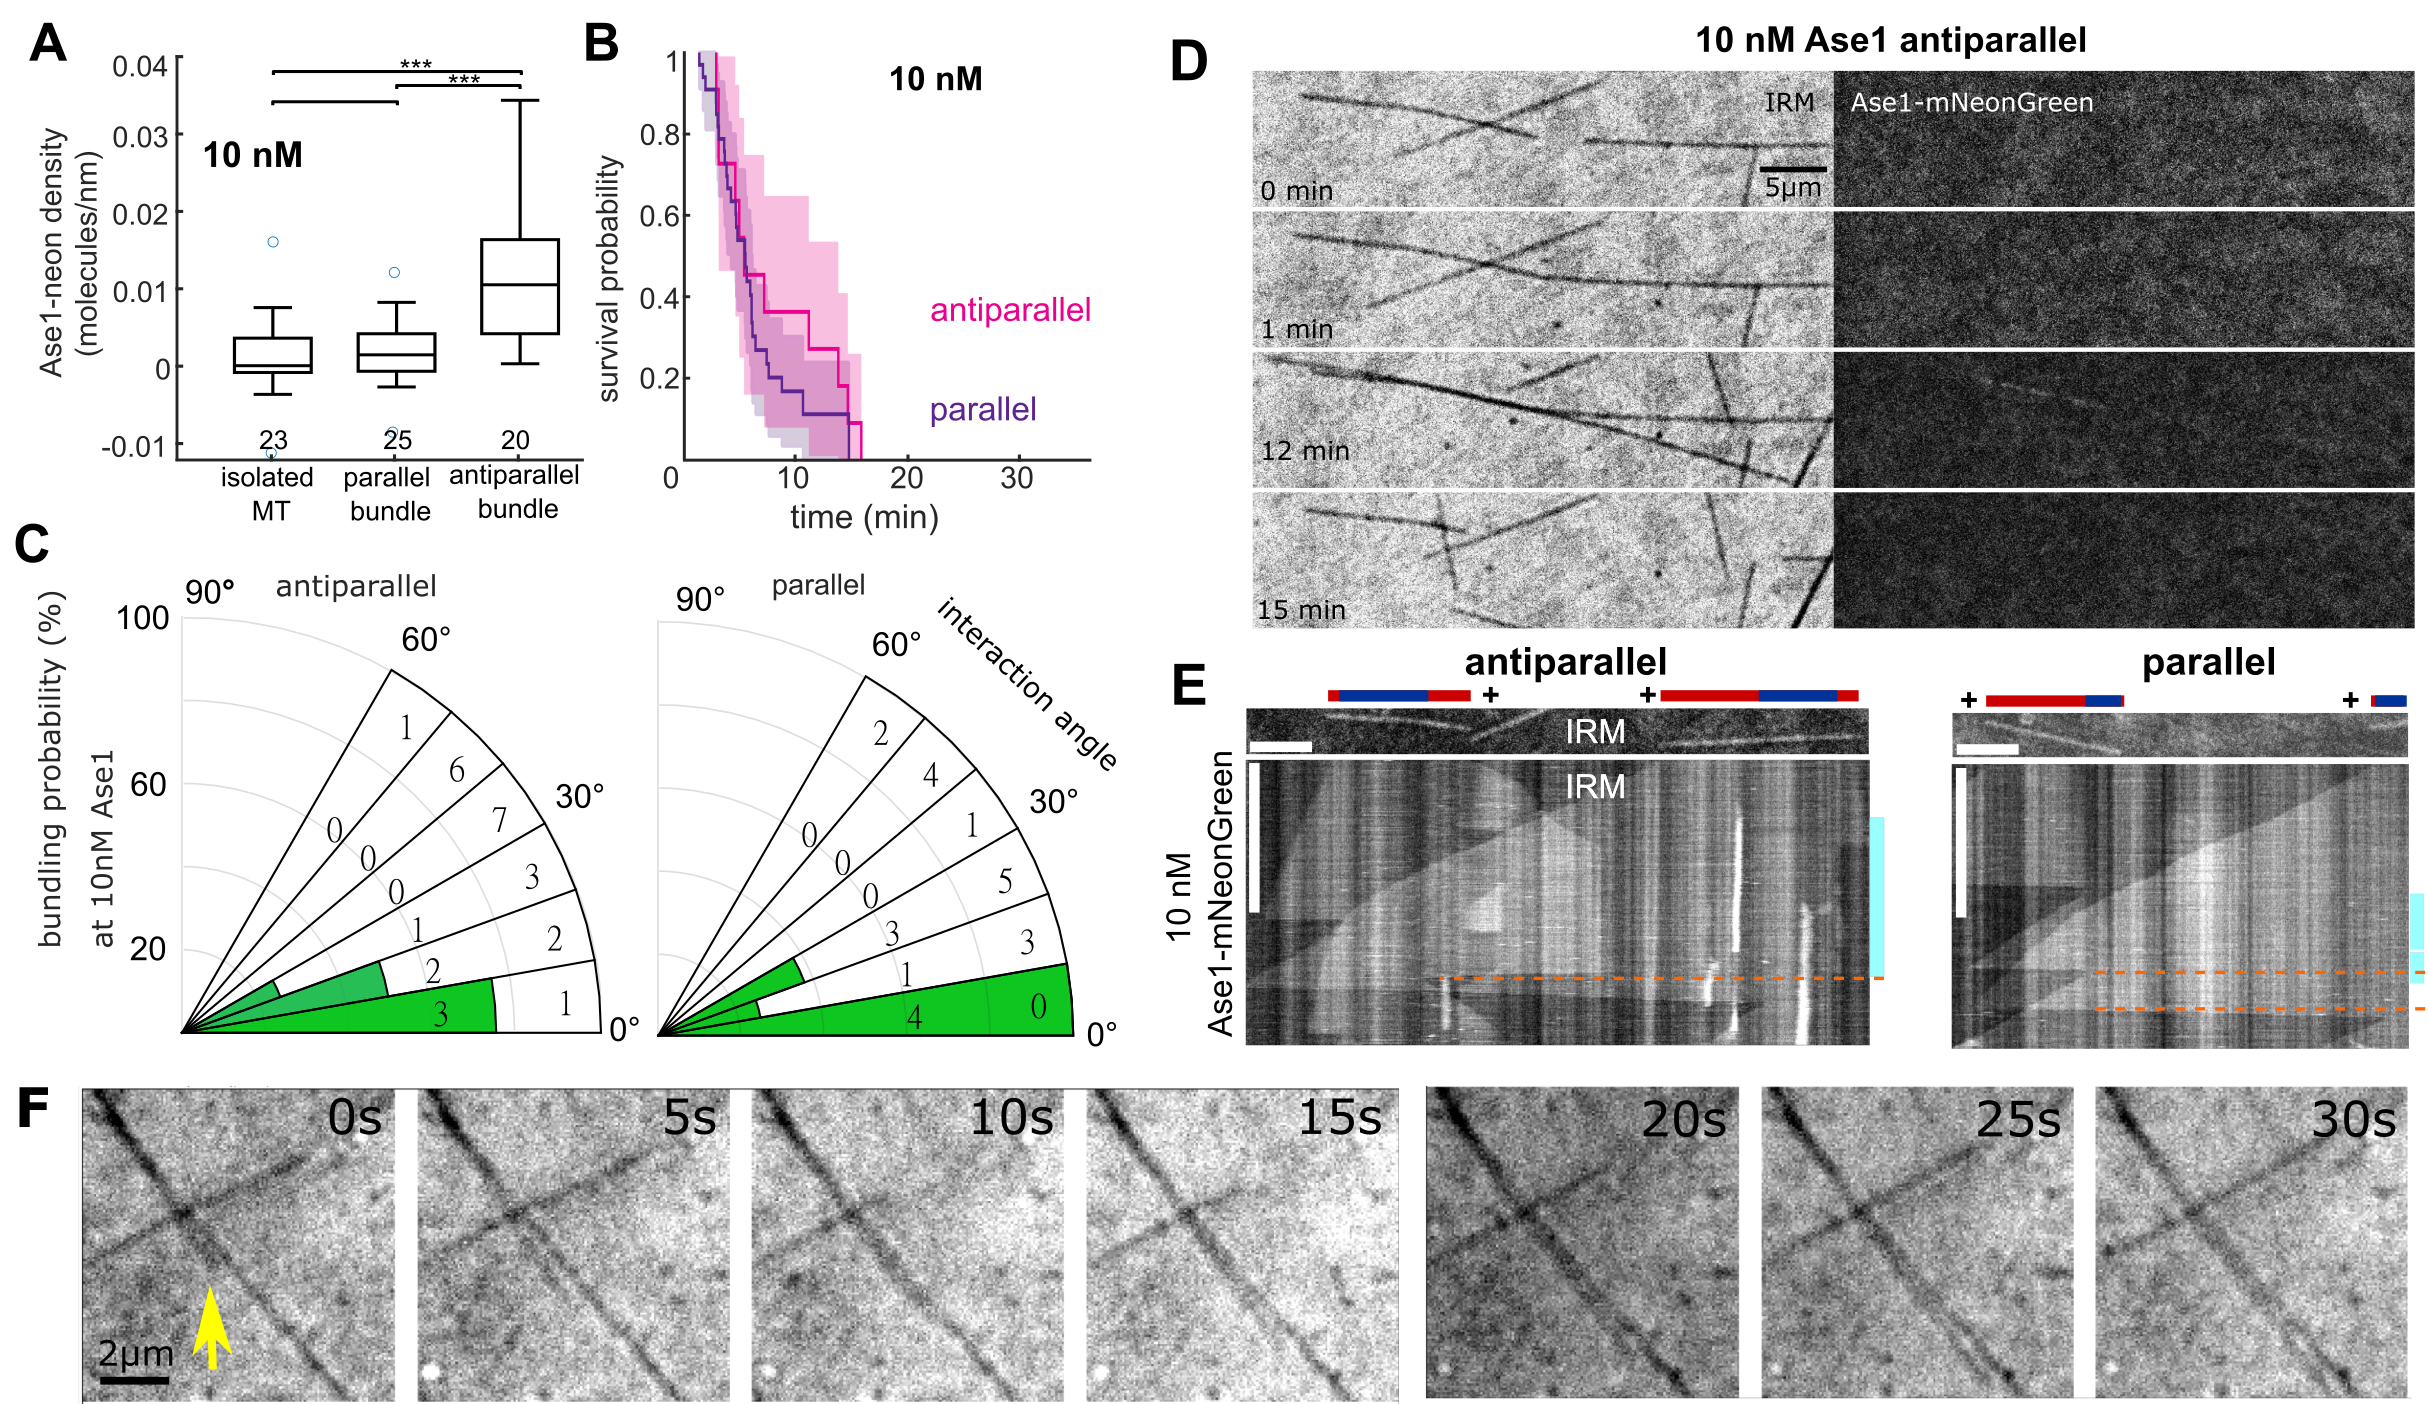
\includegraphics[width=1\linewidth]{Figures/ase1_1c.png}
    \caption[Antiparallel overlaps are not significantly stabilized at low Ase1 concentrations.]{
        (A,B) Quantifications of Ase1 densities and lifetimes for the 10nM Ase1 condition analogous to panels in \autoref{ase1b}. (C) Quantifications of bundling probabilities for the 10nM Ase1 condition analogous to \autoref{ase1a}D. (D) Snapshots of an antiparallel overlap at 10nM Ase1. (E) Kymographs for the 10nM Ase1 condition, representation analogous to \autoref{ase1a}A. The left panel shows the same event as D. (F) A microtubule polymerizing close to another, parallel microtubule at 0nM Ase1 (imaged with IRM). The tip of microtubule in question is indicated by a yellow arrow. As can be seen, no bundling is occurring despite the fact that the microtubules are very close to each other. Panels taken from \cite{Krattenmacher2024}.
        }\label{ase1c}
\end{figure}

Indeed, as indicated by the kymographs shown in \pref{ase1d}{A}, we found rescue frequencies to be increased for antiparallelly crosslinked microtubules at the Ase1 concentrations where we had observed increased lifetimes of these overlaps \pref{ase1d}{B}. To test whether Ase1 crosslinking might have other significant effects on MT polymerization, we next quantified the other three parameters of microtubule dynamic instability. We found that catastrophe frequencies were similar across the tested conditions, with no statistically significant difference between the different populations \pref{ase1d}{C}. Polymerization velocities were similar for all microtubule types, either isolated or bundled, across all tested Ase1 concentrations as well \pref{ase1d}{D}. However, at 420nM Ase1, MTs depolymerized markedly slower than at lower Ase1 concentrations. Further, at 42nM and 420nM Ase1, antiparallel MTs displayed a marked decrease in depolymerization velocity compared to isolated and parallel MTs \pref{ase1d}{E}. Thus, we observed Ase1 to only have a measurable effect on MT depolymerization, by reducing the rate of depolymerization and increasing chances for rescue, with no effect on polymerization.\par

If one only considers our results at 42nM, one could speculate that the particularly pronounced stabilization of antiparallel microtubules was due to the increased number of Ase1 molecules on antiparallel MTs as compared to parallel and isolated MTs. However, at 420nM, the number of Ase1 molecules per MT was similar across all types of MTs, while the antiparallel MTs still were more stable, despite indistinguishable Ase1 densities on antiparallel versus parallel MT overlaps \pref{ase1d}{F,G}. Thus, Ase1 engaged in antiparallel crosslinking seems to have a stronger effect on MT depolymerization than Ase1 engaged in parallel crosslinking or Ase1 not engaged in crosslinking. This deduction is supported by the fact that the number of Ase1 molecules engaged in Ase1 crosslinking was the only factor we could identify as influencing the frequency of rescues (note, however, that the number of molecules directly participating in the crosslinking process, i.e. simultaneously bound to both crosslinked microtubules, is not measurable in this assay). Notably, we with a different set of experiments ("Set B experiments," see \autoref{methods}) found the same result \autoref{ase1e}, showing the robustness of this finding: At these conditions, we observed antiparallely linked microtubules to exhibit rescues, at a density of around 0.2 molecules per nm which we at these buffer conditions had established with 1nM Ase1 \pref{ase1e}{B,C} (as a side note, the Ase1 used in these experiments was a slightly different construct, see \autoref{methods}). At these buffer conditions, isolated microtubules did not exhibit any rescues at all, even when we increased the Ase1 concentration from 1 to 6nM such that the Ase1 density on isolated microtubules was comparable to the Ase1 density on antiparallel bundles at 1nM Ase1 \pref{ase1e}{B,C}. The depolymerization velocity similarly decreased with increasing Ase1 concentration \pref{ase1e}{D}. Altogether, these results show that Ase1 can stabilize antiparallel microtubules while only having minor stabilization effects on MTs outside of such overlaps.

\begin{figure}[h]
    \centering
    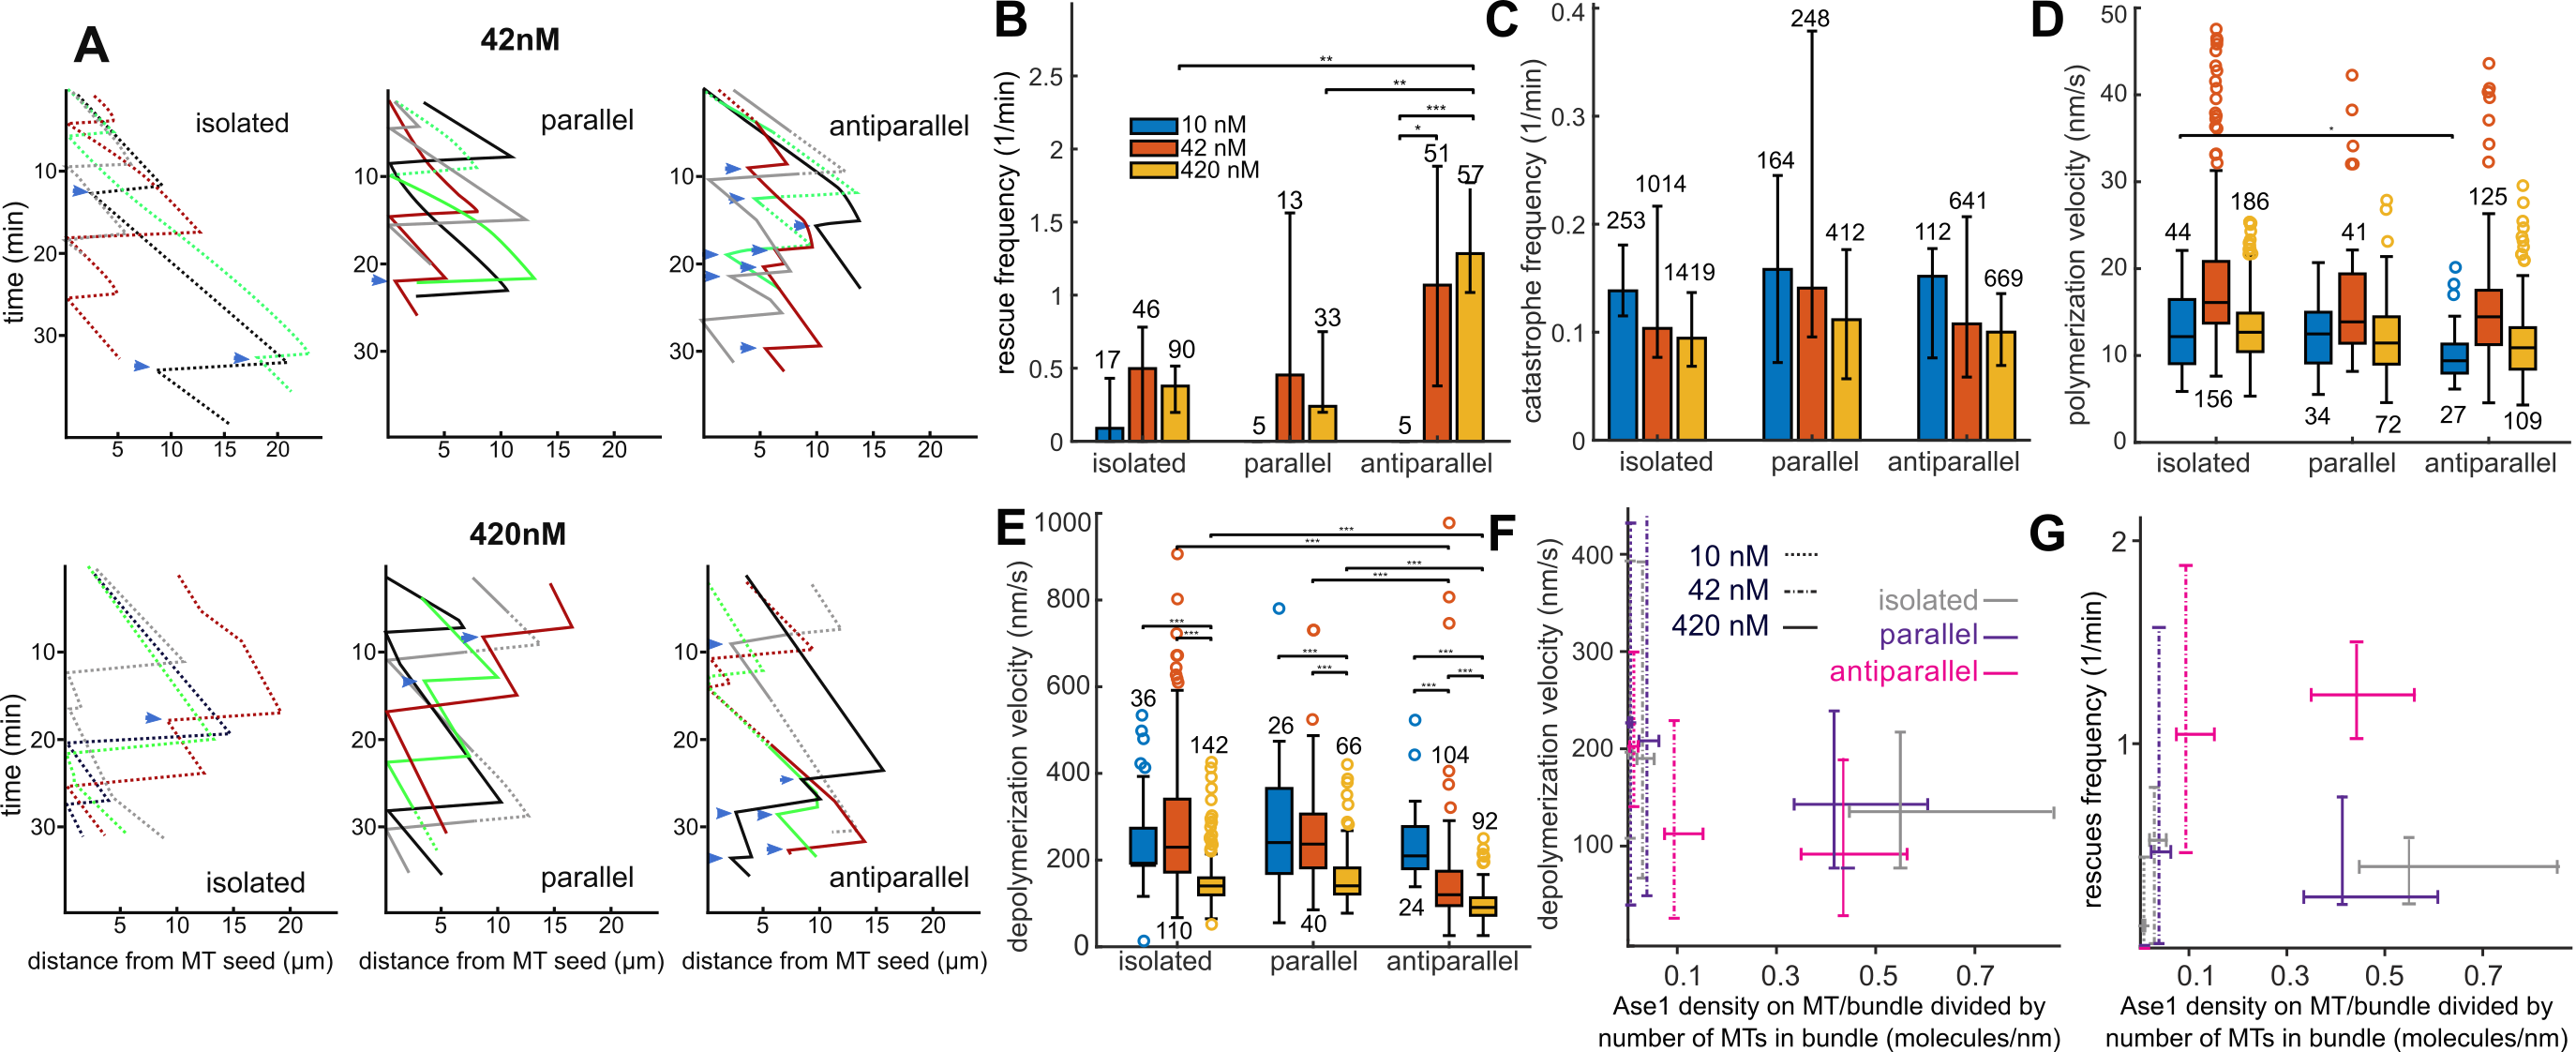
\includegraphics[width=1\linewidth]{Figures/ase1_1d.png}
    \caption[Representative kymograph traces.]{
    (A) Representative kymograph traces of the types of events we observed in our dataset which we present in \autoref{ase1a}, \autoref{ase1b} and \autoref{ase1c}A-E. Blue arrows indicate rescue events. Dotted lines indicate stretches where the MT was isolated. (B) Rescue frequency, (C) catastrophe frequency, (D) polymerization velocity, and (E) depolymerization velocity of dynamic MT plus ends in different configurations and in the presence of varying concentrations of Ase1-mNeonGreen. (F) Depolymerization velocity (see E) versus Ase1-mNeonGreen density on a given MT or bundle divided by number of MTs in that bundle (i.e., the density as shown in \autoref{ase1b}B is divided by 2 in the case of parallel and antiparallel MTs).  (G) Rescue frequency (see B) versus Ase1-mNeonGreen density (see \autoref{ase1b}B). All plots show results for the same experiments as shown in \autoref{ase1a} and \autoref{ase1b}. * p<0.05, ** p<0.01, *** p<0.001 (Tukey's test; only significance levels are visualized that share either the same MT type or the same concentration. No visual link between two populations sharing one such characteristic signifies  p>0.05. In B and C a given population comprises the frequencies recorded for the respective experiments, in D and E the velocities recorded for respective sampled periods). Boxplots are weighted by the length of a sampled period of polymerization or depolymerization. In boxplots, the numbers indicate the number of recorded events, in bar plots, the numbers indicate the sum of the length of all sampled periods of polymerization or depolymerization (in minutes). In bar plots, the height of the bar indicates the catastrophe/rescue frequency as determined from all time lapses (number of total events divided by total duration of depolymerization), while the error bars indicate the lowest and highest rates as determined from each isolated time lapse; velocities are normalized to the median velocity of isolated MTs (Methods). Panels taken from \cite{Krattenmacher2024}.
        }\label{ase1d}
\end{figure}

\begin{figure}[h]
    \centering
    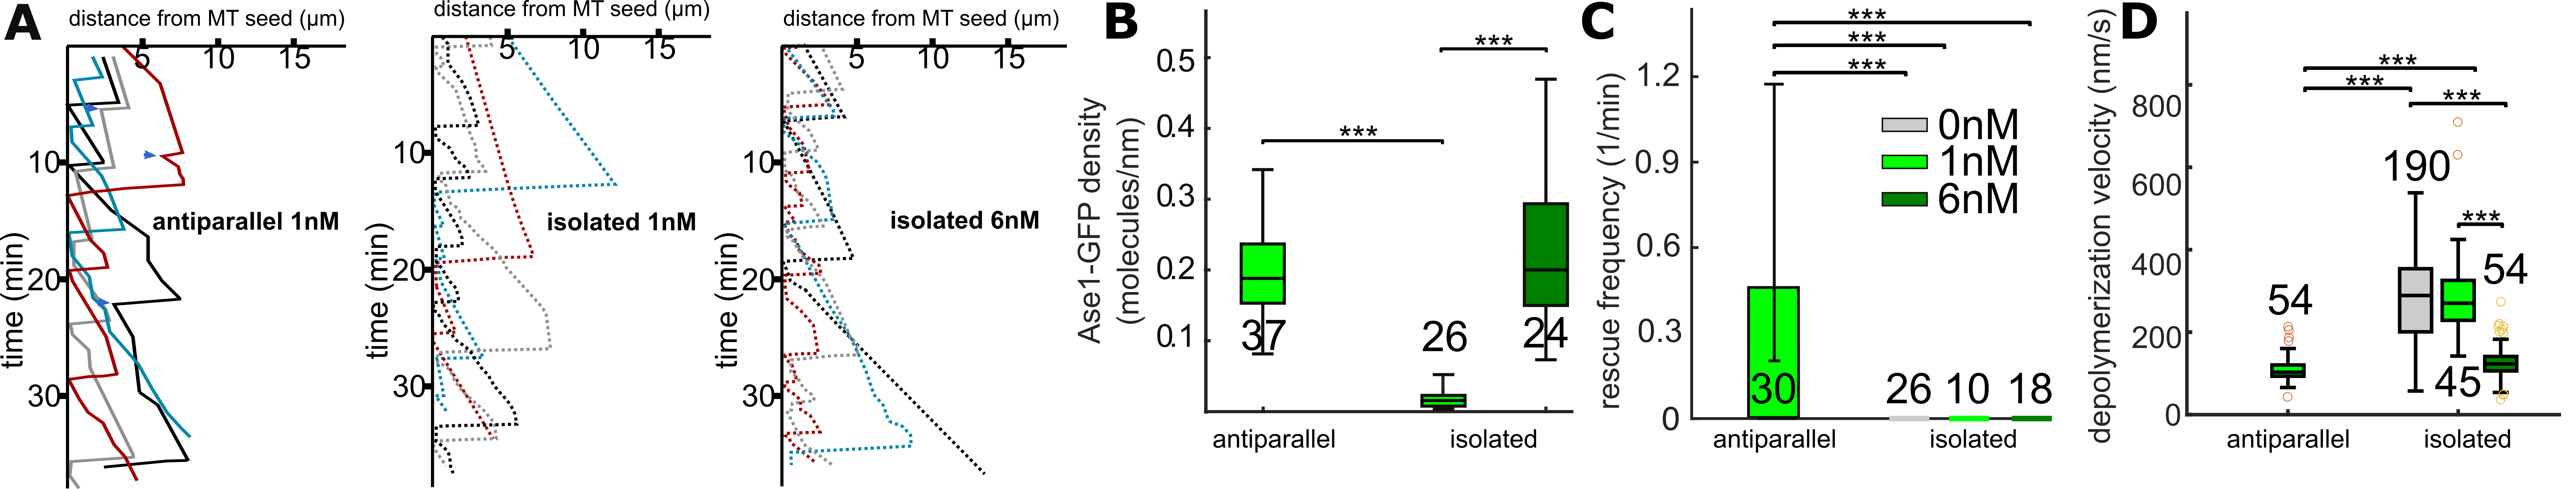
\includegraphics[width=1\linewidth]{Figures/ase1_1e.png}
    \caption[Set B experiments microtubule dynamics.]{
    Data obtained from a second set of experiments ("Set B experiments", see \autoref{methods}) with different experimental parameters than the data from the set of experiments shown thus far ("Set A experiments"). (A) Representative kymograph traces, representation analogous to \aref{ase1d}{A}. (B) Quantification of the density of Ase1-GFP(Methods). The numbers below the boxes denote the number of analyzed microtubule bundles. (C) Rescue frequency and (D) depolymerization velocity, representations analogous to \aref{ase1d}{B,E}. Legend for B-D in C, showing the concentration of Ase1-GFP in each set of experiments. Panels taken from \cite{Krattenmacher2024}, except panels C and D, which I created only for this thesis.
        }\label{ase1e}
\end{figure}

\FloatBarrier
\subsection{Interactions between Ase1 and the depolymerizing microtubule end}
\begin{figure}[h]
    \centering
    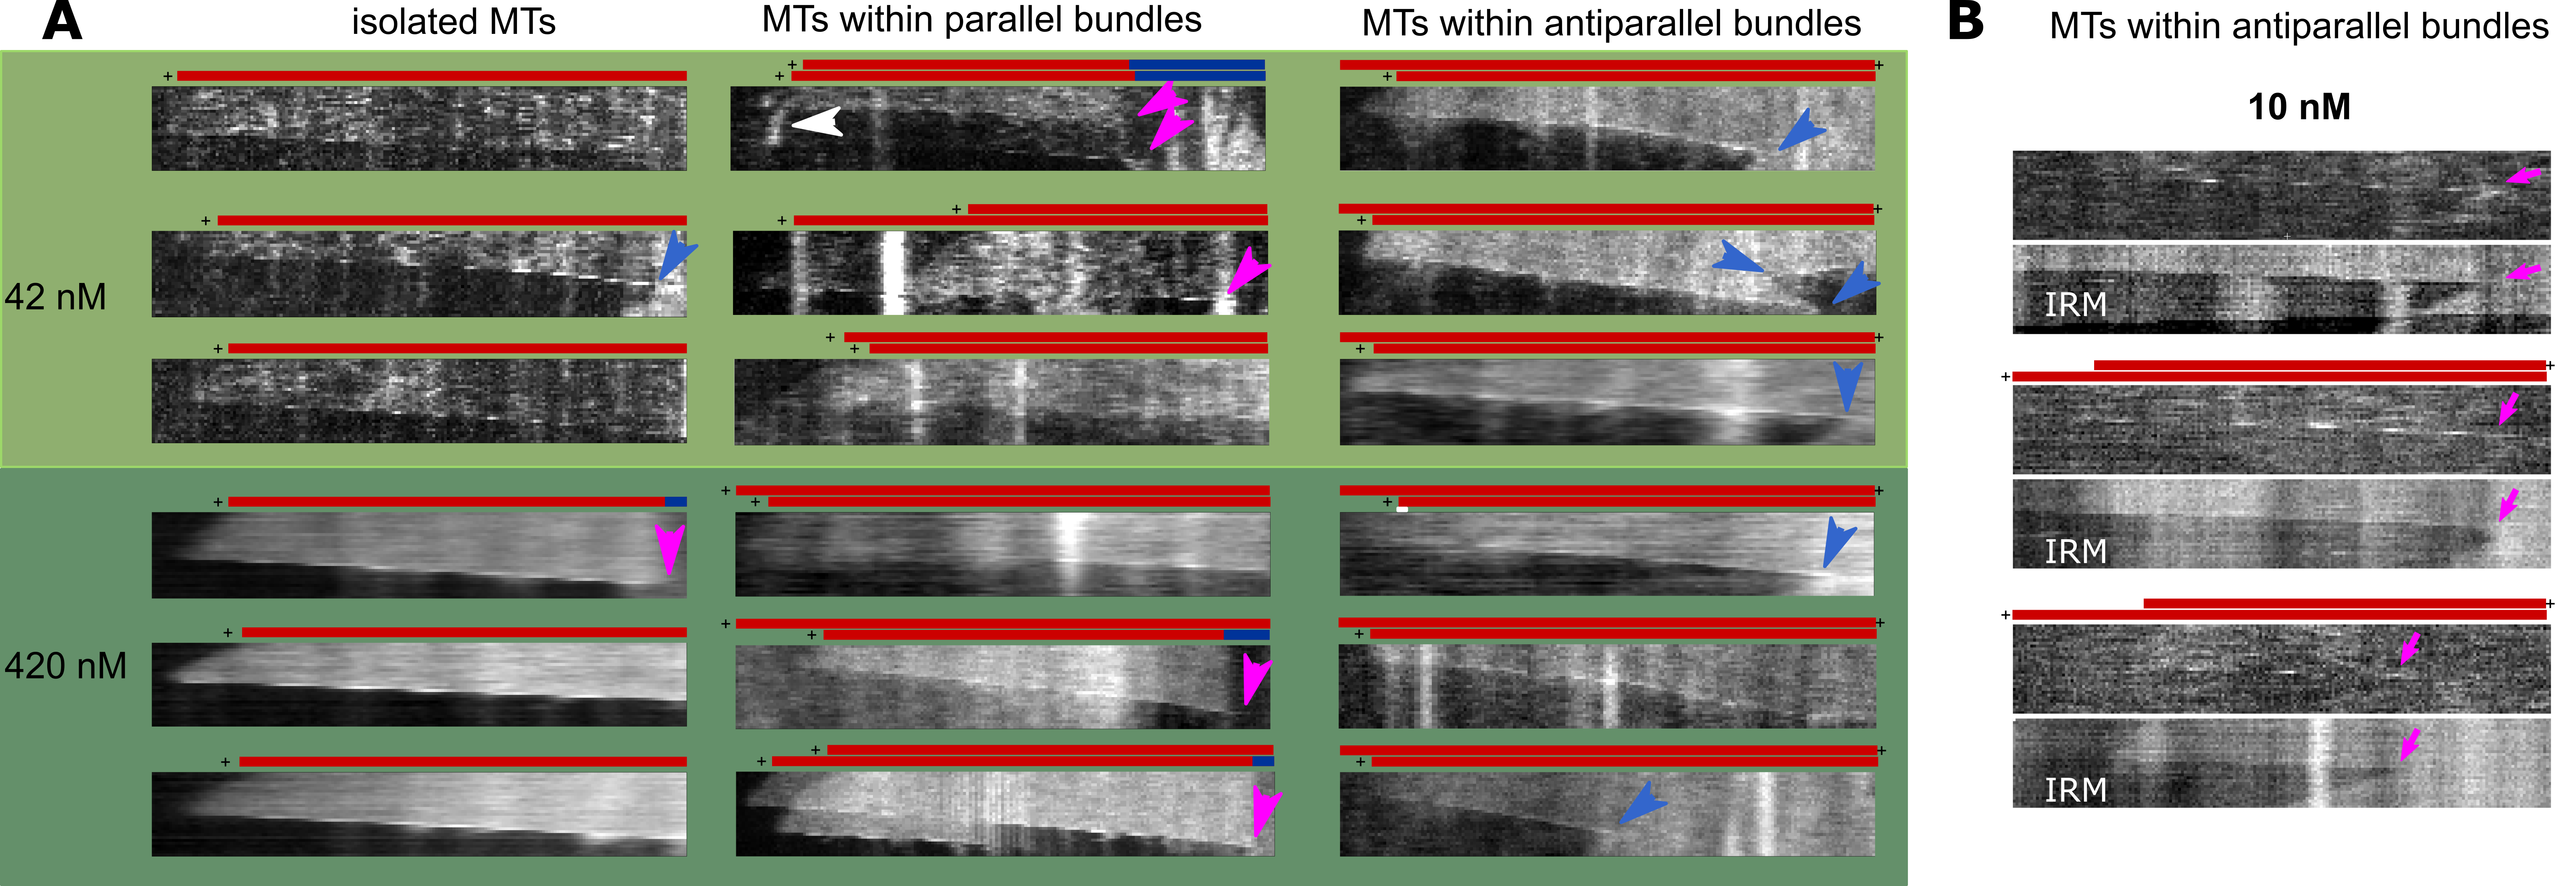
\includegraphics[width=1\linewidth]{Figures/ase2a.png}
    \caption[Set A experiments kymographs showing Ase1 herding.]{Kymographs of depolymerization events (Set A experiments as shown in \aref{ase1d}{A}). (A) Kymographs of all examined microtubule configurations at 42nM and 420nM Ase1. (B) Kymographs of events observed at 10nM Ase1 (antiparallel overlaps only since at this concentration there was no Ase1-mNeonGreen signal at the ends of parallel overlaps and isolated MTs). Each kymograph is 12 µm in width and 150 seconds in height, contrast and balance varies from panel to panel (each kymograph shows a different MT). To facilitate understanding of the kymographs, rescues are pointed out with blue arrows. Pink arrows indicate a MT tip reaching its GMPCPP seed. The white arrow indicates where one of the parallel MTs, before catastrophing, had briefly engaged in antiparallel crosslinking with another isolated MT. Where no arrows are shown, the MT continues to depolymerize toward the right. Panels taken from \cite{Krattenmacher2024}.
        }\label{ase2a}
\end{figure}
Given that we had shown that Ase1 can stabilize depolymerizing microtubules, we suspected that Ase1 molecules very likely interact directly with depolymerizing MT ends. This is indeed what we found when examining the distribution of Ase1. While Ase1 did show no preference for binding to polymerizing MT ends, the kymographs which we had generated showed that Ase1 accumulated at depolymerizing MT ends, for Set A experiments \pref{ase2a}{A,B} as well as Set B experiments \pref{ase2b}{A}. We now set out to quantify this effect. Because the data for Set B experiments allowed for a more fine-grained analysis due to a higher framerate and a more pronounced accumulation effect, we in the following limited our analysis to the Set B experimental data. Given that isolated and parallel MTs behaved very similarly in our assays (though only in Set A experiments we observed a sufficiently high number of parallel overlaps for a thorough analysis), we also chose to focus on comparing isolated and antiparallel MTs.\par
\begin{figure}[h!]
    \centering
    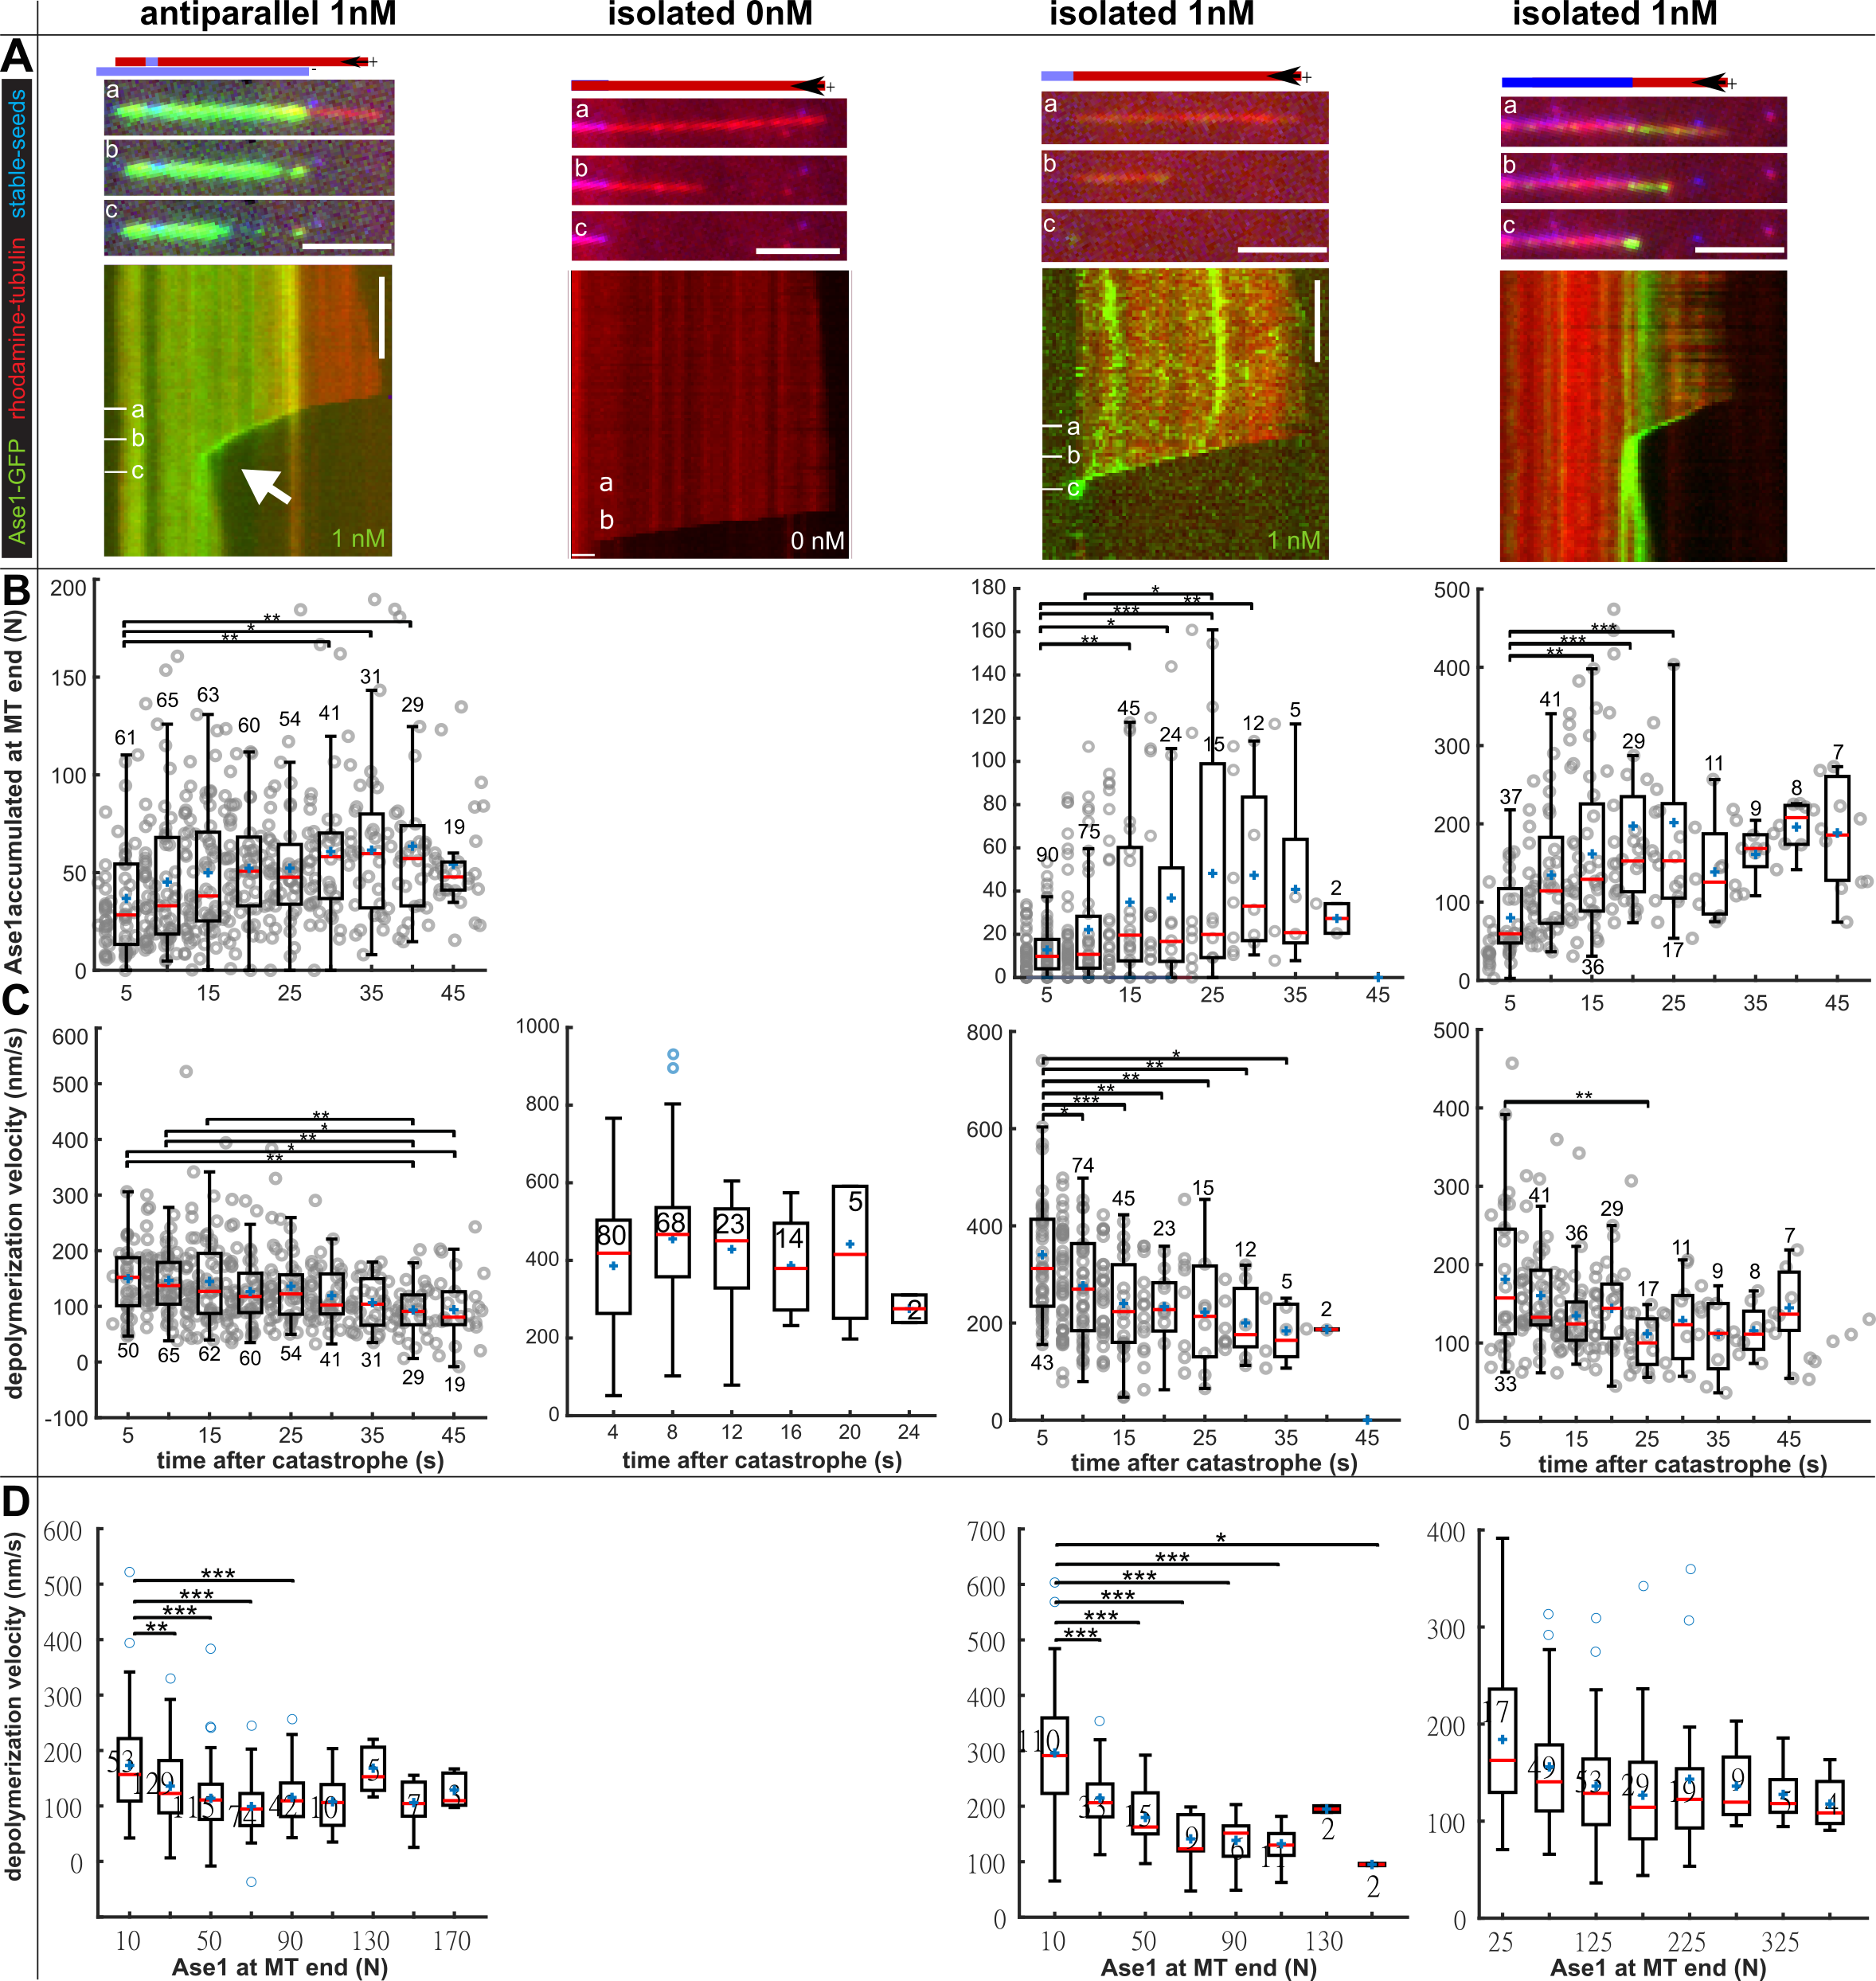
\includegraphics[width=1\linewidth]{Figures/ase2b.png}
    \caption[Ase1 accumulates at depolymerizing MT ends.]{Experimental data on herding of Ase1 (Set B experiments as shown in \aref{ase1e}{A}). (A) Kymographs of depolymerizing MTs. The stabilized GMPCPP-MT seeds were labelled with 15\% rhodamine and 15\% Alexa647 (or, alternatively, with 2\% Alexa647), while the free tubulin in solution was labelled with 7\% rhodamine. In sketches, dynamic extensions with GDP lattices are colored red, and stabilized GMPCPP seeds are colored blue or light blue (in case of the weakly-labelled seeds). The scale bars are 5 micron and 1 minute, contrast and balance vary from panel to panel (each kymograph shows a different MT). White arrows highlight rescue events. (B) The number of additional Ase1 molecules at the end of depolymerizing MTs, plotted over the time passed since the catastrophe. Each data point represents data extracted from one line scan. (C) The frame-to-frame depolymerization velocity of MTs over time (analogous to B). Because the exact time of catastrophe is unknown due to limits in temporal resolution, the velocity measurement right after catastrophe underestimates the actual velocity. (D) Instantaneous depolymerization velocity plotted over number of additional Ase1 molecules at the MT end. Panels taken from \cite{Krattenmacher2024}.
        }\label{ase2b}
\end{figure}

Our quantitative analysis of Ase1 accumulation at depolymerizing microtubule ends confirmed the visual impression given by the kymographs - Ase1 was indeed accumulating at depolymerizing MT ends, for both isolated and antiparallel MTs \pref{ase2b}{B}. In addition, the quantitative analysis also revealed that the Ase1 accumulates were growing the quickest during the early stages of depolymerization \pref{ase2b}{B}. Intuitively, one may expect that this accumulation is related to the stabilization of microtubules during depolymerization. Indeed, Ase1 accumulation correlated with a decrease in depolymerization speed \pref{ase2b}{B-D}. While this correlation does not imply a causal relationship, it does lend support to the existence of such a relationship. An alternative explanation could be a possible hidden third factor, most notably the natural slowdown of depolymerization velocity after catastrophe which has been observed by others \parencite{Luchniak2023}. In other words, it is conceivable that depolymerizing MTs accumulate Ase1 and slow down over time, and that these two phenomena are not causally related. However, in the absence of Ase1 we had not observed any slowdown in MT depolymerization comparable to what we observed in the presence of Ase1 \pref{ase2b}{C}. \par

\begin{figure}[h]
    \centering
    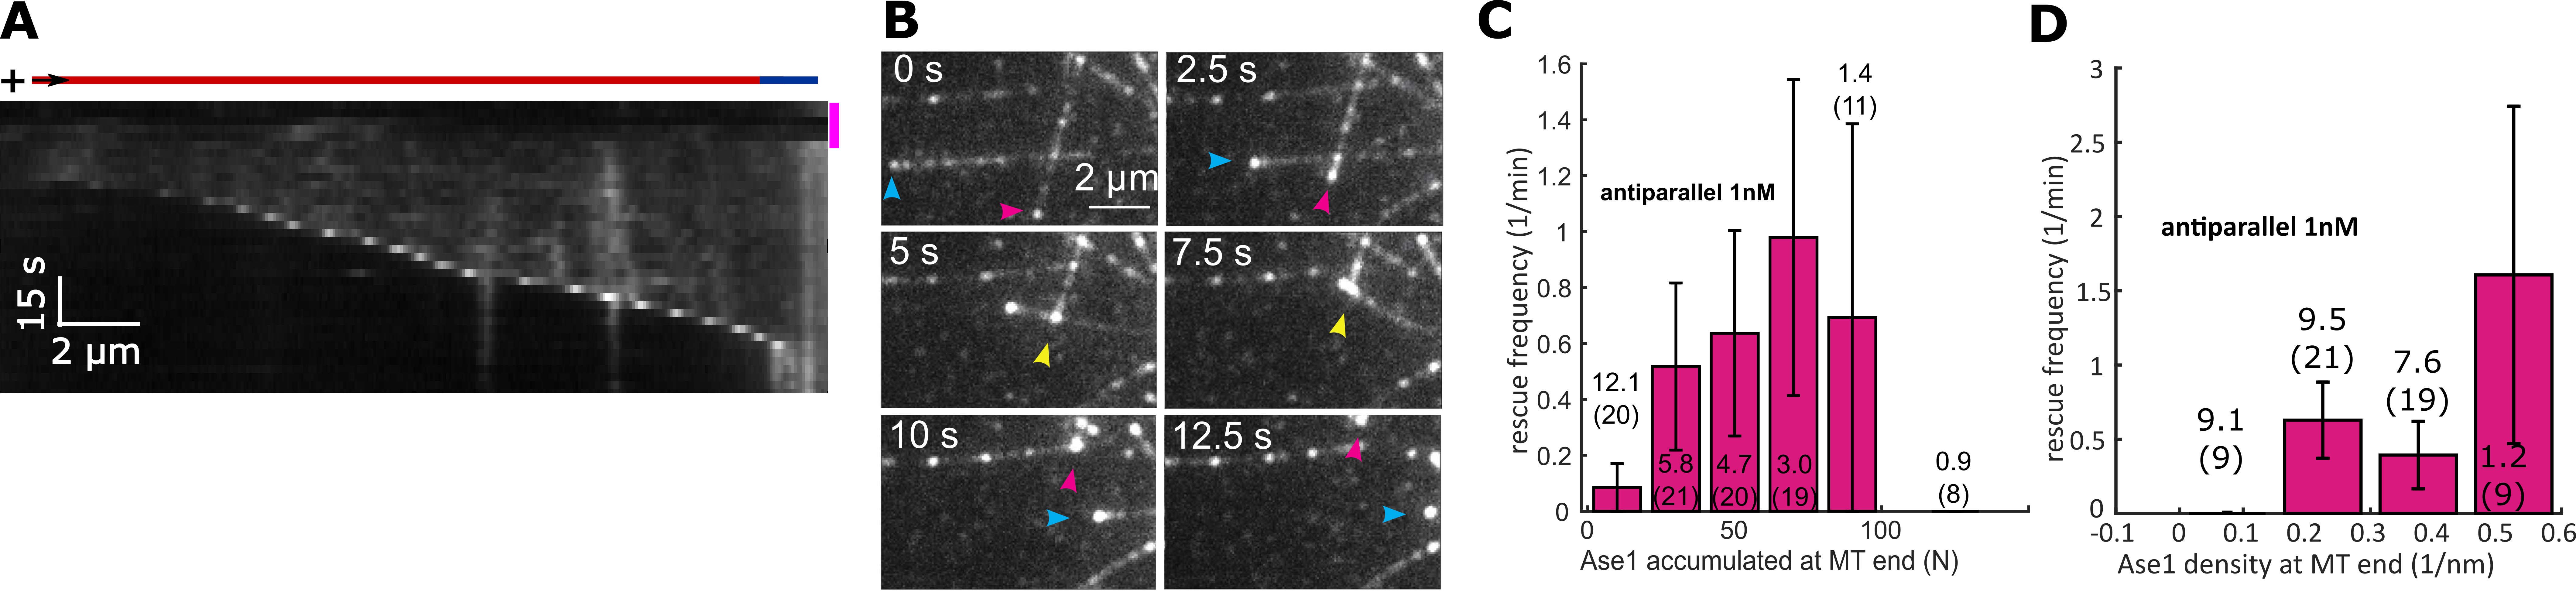
\includegraphics[width=1\linewidth]{Figures/ase2c.png}
    \caption[Ase1 is herded by depolymerizing MTs.]{
    (A) Kymograph (Ase1-mNeonGreen channel) of depolymerizing MT. In this experiment, Ase1 and tubulin had been removed from the assay buffer during the time frame indicated by the pink bar next to the kymograph, prompting subsequent MT depolymerization and concomitant Ase1 accumulation at the end. (B) Time series of micrographs (Ase1-GFP channel) showing an event where the accumulated Ase1 at one depolymerizing MT end (indicated by red arrows) causes the end to “drag” a MT it crosses with it, thereby bending it (yellow arrows). The blue arrows indicate the (depolymerizing) end of the MT before and after it got bent. (C) Rescue frequency plotted over number of additional Ase1 molecules at the MT end. The duration depolymerized at a respective x-value was added to the respective bin. The number of rescues observed in the same bin (N) was then divided by the sum of depolymerization durations (shown in min, the number in parentheses refers to the number of MTs) to estimate the rescue frequency. The correlation coefficient (weighted \parencite{Pelletier2024} by sums of depolymerization durations) is 0.67. The total length of a given error bar equals two times the square root of the number of the rescues in the corresponding bin divided by the sum of the time depolymerized in the corresponding bin. (D) Rescue frequency plotted over the height of the peak of the Ase1 density at the MT end (the weighted correlation coefficient is 0.76). Representation analogous to C. C and D show data from Set B experiments. Panels taken from \cite{Krattenmacher2024}.
        }\label{ase2c}
\end{figure}

Our findings so far suggested that we observed "herding" of Ase1 by the depolymerizing MT end, a phenomenon which has recently been reported for a synthetic MT crosslinker \parencite{Drechsler2019}. To confirm this, we needed to exclude the possibility that Ase1 specifically tracks depolymerizing MT ends by having a higher affinity for depolymerizing MT regions. We thus performed an experiment where we removed both Ase1 and tubulin from solution after first having polymerized Ase1-decorated MTs. We found Ase1 to still accumulate at the ends of depolymerizing MT \pref{ase2c}{A}, indicating that the accumulates are indeed comprised of Ase1 molecules that were already bound to the MT lattice before catastrophe had occurred. As reported for the synthetic polymer \parencite{Drechsler2019}, we also observed instances of depolymerizing MT ends which herded Ase1 molecules pulling on other MTs \pref{ase2c}{B}. This indicates that substantial forces can be transmitted via Ase1 herding.\par

What is the impact of Ase1 herding on microtubule depolymerization for isolated versus antiparallel MTs? Again, we found that the impact of single Ase1 molecules on the depolymerization of antiparallel MTs is stronger than in the case of isolated microtubules: While isolated microtubules at 6nM Ase1 herded more Ase1 than antiparallel microtubules at 1nM Ase1, they did not depolymerize more slowly than antiparallel MTs \pref{ase2b}{B,C}. For antiparallel MTs, we also observed the number of herded Ase1 molecules to positively correlate with the probability of a rescue occuring \pref{ase1c}{C} (a phenomenon we could not test for isolated MTs since they did not exhibit any rescues in this dataset; furthermore, the rescue frequency of isolated MTs appears independent from Ase1 density, see \aref{ase1d}{B}). Moreover, the Ase1 density at the microtubule end, which is a measure for not only accumulated Ase1 but the total number of Ase1 molecules present at the end, also shows a positive correlation with rescue frequency \pref{ase1c}{D}.\par

\begin{figure}[h!]
    \centering
    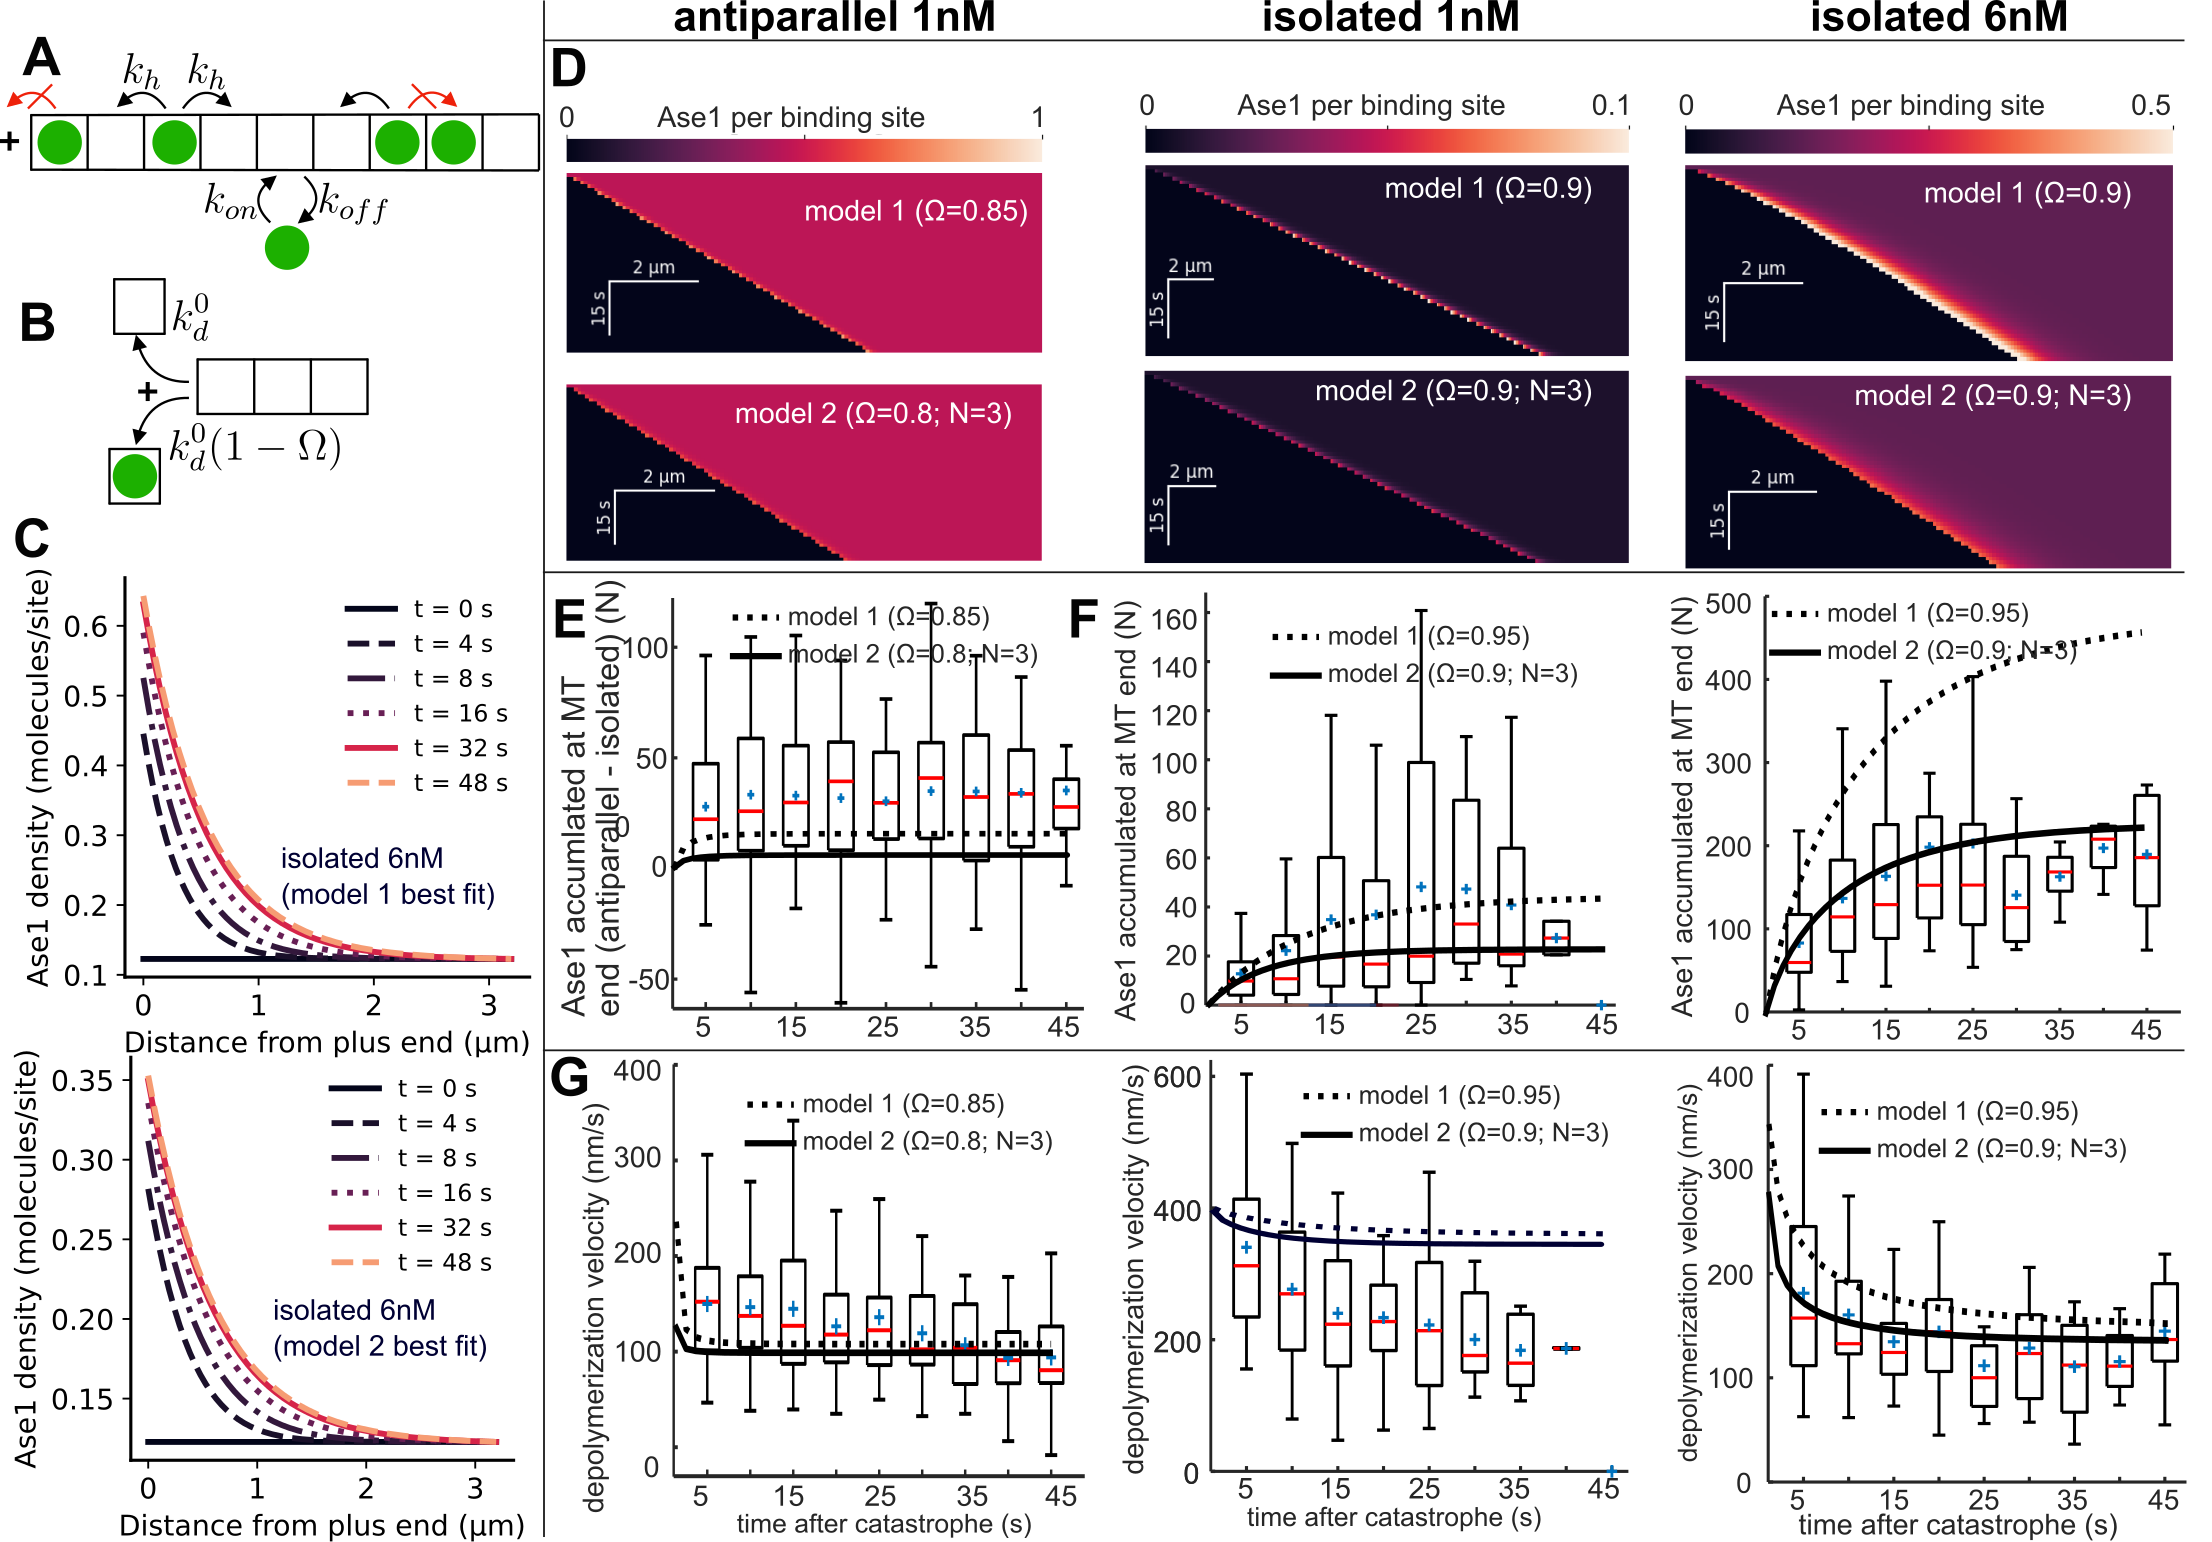
\includegraphics[width=1\linewidth]{Figures/ase2d.png}
    \caption[Modeling of Ase1 herding - results.]{
    (A,B) Cartoons representing model assumptions (see Methods): (A) Ase1 binding, unbind, and hopping to neighboring sites are stochastic events with constant rates $k_{on},k_{off},k_h$. Only one Ase1 molecule can be attached to any one tubulin heterodimer, so moving or binding to an occupied binding site is not allowed (red crossed arrow on the right). Ase1 does not fall off from the MT by hopping at its plus ends (red crossed arrow on the left). (B) In Model 1, we assume that the detachment rate of the tubulin terminal subunit is $k_d^0$ when the first tubulin subunit is free of Ase1, and $k_d=(1-\Omega)k_d^0$ if Ase1 is bound at the terminal site (for Model 2, see Main Text and Methods). (C) Distribution of Ase1 density on terminal sites in time for the indicated timepoints (see legend) as predicted by Model 1 (A) and 2 (B) with model parameters as in F (right panel). (D-G) Modelling results for Model 1 and Model 2 with N=3 (for both models, 3 PFs had been assumed to be engaged in crosslinking in the case of antiparallel MTs, see Methods). Experimental data is presented in the form of boxplots. (D) Distribution of Ase1 density in time represented as a simulated kymograph (see scalebars; in the case of antiparallel MTs, values are for the PFs engaged in crosslinking, the other PFs are assumed to have 0 coverage). (E) Number of crosslinked Ase1 molecules plotted versus time after catastrophe. As an estimate of the number of crosslinked Ase1 molecules, the plot shows the following on the y-axis: The number of additional Ase1 molecules at the end of a depolymerizing antiparallel MT at a given time \pref{ase2b}{B, left panel} minus the median number of additional Ase1 molecules at the ends of isolated MTs in the same experiment as a given antiparallel MT (at the same time after catastrophe) \pref{ase2b}{B, mid panel}. (F,G) Values of Ase1 accumulation and depolymerization velocity at steady state derived from experiments (boxplots) or predicted by Model 1 and 2 (lines). The boxplots in F and G are the same as in the corresponding plots in \aref{ase2b}{}. Panels taken from \cite{Krattenmacher2024}.
        }\label{ase2d}
\end{figure}

\begin{wrapfigure}{l}{0.3\textwidth}
    \centering
    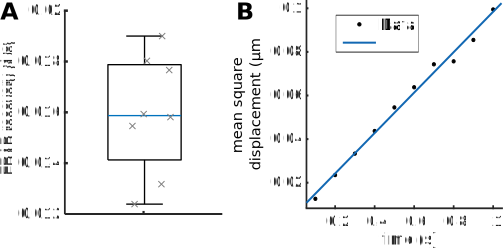
\includegraphics[width=1\linewidth]{Figures/ase2FRAP.png}
    \caption[Experimental determination of the diffusion coefficient and off-rate of Ase1.]{
    (A) Recorded FRAP recovery times on isolated MTs (see Methods) – the median value was used as $k_{off}$ for modelling. (B) Mean square displacement of single Ase1 molecules diffusing on isolated MTs during the first second of their interaction with the MT (see Methods) and fitted line – the slope of the fitted line $D$ was used for modeling ($kh = Da^2$, with $a$ being the tubulin dimer length) (number of molecules = 2008). Panels taken from \cite{Krattenmacher2024}.
        }\label{ase2FRAP}
\end{wrapfigure}

Our experiments thus demonstrate that lattice-bound Ase1 molecules are herded by the depolymerizing MT ends and that the number of swept Ase1 molecules correlates with reduced depolymerization velocity, and, for antiparallel overlaps, with an increased probability of rescue. Yet how do these effects relate to each other? We set out to tackle this question by mathematically modeling Ase1 herding, focusing on the relation between depolymerization velocity and Ase1 accumulation. We thus developed a simple mathematical model that considers a one-dimensional MT made of lattice sites corresponding to tubulin heterodimers, starting at the plus end (see Methods). The model neglects the interaction between protofilaments, and for simplicity focuses on the effect of Ase1 on the depolymerization velocity of isolated MTs. Events such as Ase1 binding, unbinding, and hopping to neighboring sites are stochastic with constant rates $k_{on},k_{off},k_h$ \pref{ase1d}{A} that were determined experimentally (\aref{ase2FRAP}{}, \aref{ase2t1}{}). Importantly, only one Ase1 molecule can be attached to any one tubulin heterodimer, and Ase1 can thus only hop to unoccupied neighboring sites. We also assume that Ase1 does not fall off from the MT by hopping at its plus ends, as shown experimentally \parencite{Braun2011}. MT depolymerization is modelled stochastically by detachment of the terminal subunit, at a rate that is affected by Ase1 \pref{ase1d}{B}. Specifically, this rate is $k_d^0$ when the first tubulin subunit is free of Ase1, and $k_d=(1-\Omega)k_d^0$, if Ase1 is bound at the terminal site. The value of $k_d^0$ is set by the MT depolymerization velocity in the absence of Ase1, measured experimentally \pref{aset1}{}. The parameter $\Omega\in[0,1]$ specifies the effect of Ase1 on depolymerization. If $\Omega=0$, Ase1 has no effect, while if $\Omega=1$, the terminal subunit cannot unbind if Ase1 is bound. For any value $\Omega>0$, this simple model leads to an exponentially-declining accumulation of Ase1 near the depolymerizing end \pref{ase1d}{C}. The accumulation occurs because subunits without Ase1 are more likely to be lost at the plus-end, so depolymerization increases the density of Ase1 at the depolymerizing end. At steady state, the system can be characterized by the probability $P_1$ of the terminal site to be occupied, and the rate of subunits loss is $k_d=k_d^0 (1-\Omega P_1)$.\par

\begin{table}[!ht]
    \centering
    \begin{tabular}{|l|l|l|l|}
    \hline
    \makecell{Parameter} & \multicolumn{2}{l|}{Value(s)} & Source \\ \hline
    \makecell{MT depolymerization\\ rate at 0 Ase1} & \multicolumn{2}{l|}{rate equivalent of 400 nm/s} & \aref{ase2b}{C, mid panel} \\ \hline
        Ase1 off-rate ($k_{off}$) & \multicolumn{2}{l|}{0.016 s$^{-1}$} & \aref{ase2FRAP}{A} \\ \hline
        \makecell{Ase1 diffusion\\ coefficient,\\ isolated MTs} & \multicolumn{2}{l|}{0.09 µm$^2$/s} & \aref{ase2FRAP}{B} \\ \hline
        \makecell{Ase1 diffusion\\ coefficient,\\ antiparallel MTs} & \multicolumn{2}{l|}{0.011 µm$^2$/s} & \makecell{8 times lower than isolated MTs\\ \parencite{lanskydiffusible2015}} \\ \hline
        \multirow{3}*{Ase1 on-rate ($k_{on}$)} & Isolated 1nM & 0.00012 $s^{-1}$ & \multirow{2}*{\makecell{Calculated from experimentally\\ measured $k_{off}$ and equilibrium\\ density on MT body\pref{ase1e}{B}}} \\ \cline{2-3}
         & Isolated 6nM & 0.00224 s$^{-1}$ &  \\ \cline{2-3}
         & Antiparallel (3 protofilaments) & 0.01369 s$^{-1}$ &  \\ \hline
         \makecell{Tubulin\\ dimer/binding site\\ length ($a$)} & \multicolumn{2}{l|}{8nm} & \cite{Song1995} \\ \hline
    \end{tabular}
    \caption[Model parameters that are experimentally constrained.]{Model parameters that are experimentally constrained.}\label{ase2t1}
\end{table}

\begin{table}[!ht]
    \centering
    \begin{tabular}{|l|l|l|l|}
    \hline
        Measurement & \multicolumn{2}{l|}{Value and 95\% confidence interval} & Source \\ \hline
        \multirow{3}*{\makecell{Timescale of\\ accumulation ($\tau$)}} & Isolated 1nM & 6.1 s [3.5 s, 11.4 s] & \multirow{6}*{\makecell{Fit of data shown\\ in \aref{ase2d}{E,F}\\ to\\ $A_{end}(1-e^{-t/\tau})$}} \\ \cline{2-3}
         & Isolated 6nM & 7.2 s [5.5 s, 11.4 s] &  \\ \cline{2-3}
         & Antiparallel & 2.4 s [1.2 s, 4.9 s] &  \\ \cline{1-3}
        \multirow{3}*{\makecell{Molecules accumulated\\ at steady state,\\ per MT ($A_{end}$)}}  & Isolated 1nM & 22 [17, 29] &  \\ \cline{2-3}
         & Isolated 6nM & 185 [160, 247] &  \\ \cline{2-3}
         & Antiparallel & 31 [24, 41] &  \\ \cline{1-4}
        \multirow{3}*{\makecell{Depolymerization\\ velocity at\\ steady state}} & Isolated 1nM & 226 nm/s [194 nms/s, 254 nm/s] & \multirow{3}*{\makecell{Average value after\\ 20 seconds of\\ depolymerization}} \\ \cline{2-3}
         & Isolated 6nM & 137 nm/s [122 nm/s, 151 nm/s] &  \\ \cline{2-3}
         & Antiparallel & 117 nm/s [108 nm/s, 125 nm/s] &  \\ \hline
    \end{tabular}
    \caption[Experimental measurements that are compared with model predictions.]{Experimental measurements that are compared with model predictions. Confidence intervals (95\%) are calculated with the bootstrap method (see Methods).}\label{ase2t2}
\end{table}

All parameters of this model (Model 1) were set from experimental measurements except for $\Omega$. Therefore, we tested whether any value of $\Omega$ could quantitatively recapitulate the experimental behavior of isolated MTs with 6nM of Ase1. Specifically, we aimed to reproduce the timescale of accumulation of Ase1, and the total amount of Ase1 accumulated and depolymerizing velocity reached at steady state \pref{aset2}{}. For $\Omega=0.95$, the model predicted depolymerization velocities comparable to the ones observed experimentally \pref{ase1d}{G, right panel}, but the timescale and number of Ase1 molecules accumulated at steady state were respectively two and three times higher than experimentally observed \pref{ase1d}{F, right panel}. Therefore, despite recapitulating the experimental phenomenology qualitatively \pref{ase1d}{D, right panel}, this first model was insufficient to quantitatively reproduce our experimental results.\par

The failure of Model 1 indicated that Ase1 should affect MT depolymerization at lower density. We thus hypothesized that Ase1 molecules located at lattice sites other than the terminal one could affect depolymerization. Therefore, we tested the possibility that the rate of tubulin subunits loss at the plus end would be reduced by a factor $(1-\Omega)$ if any of the N terminal sites were occupied. This rate at steady state would then be $k_d=k_0^d [1-\Omega{1-\Pi_(i=1)^(i=N)(1-P_i)}]$, where $P_i$ is the probability of site i being occupied by Ase1. N is not experimentally constrained, but the range of possible values is small, since it is unlikely that distant tubulin subunits could affect the detachment of the terminal subunit. For $N=3$ and $\Omega=0.9$ this model (Model 2) reproduced MT depolymerization velocity and Ase1 accumulation at steady state and Ase1 accumulation timescale (Figure 5E-F), and recapitulated the dynamics of the system (Figure 5G, H). The model predicts that at steady state Ase1 density should decay exponentially from the plus end with a length scale of around 600nm (Figure S5B). Experimentally, we observed a decay of Ase1 signal from the plus end with length scale of around 200 nm (Figure S5G). However, this signal is hardly comparable with our isolated-protofilament model, not only because it comes from multiple protofilaments that may not be in register, but also because shrinking protofilaments are likely curved outwards (McIntosh et al., 2008).\par

Using Model 2 with the same value of $\Omega=0.9$, we could recapitulate the Ase1 accumulation timescale and steady state accumulation in isolated MTs with 1nM of Ase1 (Figure S5D), but the model predicted a ~15\% decrease with respect to the maximum velocity while the experimentally observed decrease was between 27\% and 36\% (Figure S5C, \aref{aset2}{}). The reason for this disagreement is likely the low density of Ase1 molecules at 1nM concentration (<1\% of tubulin dimers bound to Ase1 in the body of isolated MTs vs. ~12\% at 6nM of Ase1). At this very low density, the stochasticity of the system may not be well captured by our mean field approach (see Methods). The model also fails to reproduce the behavior of antiparallel overlaps (Figure S4E-F). This is not surprising given that overlaps are not symmetric, and some protofilaments have almost no Ase1, while others have extremely high Ase1 density (76\% tubulin dimers bound to Ase1 in the MT body assuming 2 protofilaments crosslinked, 50\% assuming 3, see “Mathematical modelling” in Methods). A more complex model accounting for protofilament interactions would be needed for overlaps, but it would need to be informed by experimental measurements of such interactions. However, it is also possible that we simply are overestimating the number of Ase1 molecules herded by antiparallel MTs, because part of the Ase1 which is lost at the depolymerizing MT end presumably remains bound to the template MT, an effect which we do not account for in our estimation. A likely expression of this effect is our observation that while at the ends of isolated MTs, we observed a (blurred) right-sided exponential decay of additional Ase1 density as predicted by our model, the additional Ase1 density at the ends of antiparallel MTs were more reminiscent of a gaussian (Figure S5J).\par
In summary, our simple model shows that the necessary assumption that Ase1 prevents depolymerization at plus ends is sufficient to explain sweeping at shrinking microtubule ends without further assumptions. Subunits without Ase1 are more likely to be lost at the plus-end, so depolymerization increases the density of Ase1 at the depolymerizing end. The model recapitulated quantitatively the behaviour of the system for 6nM of Ase1, and within an order of magnitude for 1nM of Ase1. However, a more complicated model may be required to explain the behaviour of MT overlaps.



\begin{figure}[h]
    \centering
    
\includegraphics[width=1\linewidth]{Figures/ase2e.png}
    \caption[Difference between the distribution of Ase1 on antiparallel and isolated MTs.]{
    (A) Fitting results for the lengthscale of the exponential decay $\lambda$ for all fitted density profiles $D_A $(as described in the methods). *** p<0.001 (Tukey's test). (B) An example Ase1 density profile $D_A$ and visualized fitting results for an antiparallel overlap midway during depolymerization. The microtubule seed is on the left, and depolymerization proceeds toward the left. The yellow region shows the fitted region between $X_{Dsleft}$ and $X_{Dsright}$ (Methods). (C) An example Ase1 density profile $D_A$ visualized fitting results for an isolated MT midway during depolymerization (representation analogous to B). (D) The number of accumulated Ase1 molecules as determined by the exponential (plus error function) fit divided by the number of accumulated Ase1 molecules as determined by the gaussian (plus error function) fit (numbers as determined for each respective density profile). Panel A taken from \cite{Krattenmacher2024}, the others I created only for this thesis.
        }\label{ase2e}
\end{figure}

Within a few hundred nanometers at the depolymerizing ends of antiparallel overlaps and isolated MTs, we observed accumulation of Ase1 molecules (Figure 3A,B, Figure S3D).
	\chapter{Discussion}
\section{Tau}
\input{Content/Tau_discussion}
\section{Ase1}
In this study, we examined how the diffusible MT crosslinker Ase1 affects MT depolymerization, both when connecting MTs and on individual MTs. Our findings indicate that Ase1 reduces MT depolymerizing speeds and selectively enhances rescue frequencies of MTs in antiparallel configurations, thereby stabilizing antiparallel overlaps while having minimal impact on parallel overlaps or isolated MTs. In bipolar MT arrays like the mitotic spindle, this attribute of Ase1 could enable a selective stabilization of the array's central regions, while keeping the rest of the array dynamic and pliable.\par


An earlier study on a plant Ase1 analogue, MAP65-1, found increased rescue rates of MTs within bundles compared to isolated MTs \parencite{Stoppin-Mellet2013}. This study, however, did not experimentally distinguish between parallel and antiparallel bundles. Our methods allowed us to directly distinguish between different bundling orientations, and our findings in fact support the modeling-based findings by \parencite{Stoppin-Mellet2013}. However, our results do not rule out that under different experimental conditions, Ase1 may also stabilize parallel bundles to some degree.\par

We observed Ase1 sweeping, the accumulation of lattice-bound, diffusible Ase1 at the retracting ends of depolymerizing MTs, and found that accumulated Ase1 can transduce forces to other MTs. This phenomenon, also known as "protein sweeping" or "herding," is analogous to the in vitro behavior of the MT-severing enzyme spastin and the kinetochore-associated Ndc80 and Dam1 complexes, which crosslink chromosomes to depolymerizing MT ends \parencite{Franck2007, umbreit2012ndc80, grishchuk2017biophysics}, indicate that, analogously to Dam1- and Ndc80- complexes, Ase1 accumulation at depolymerizing MT ends, antagonizes the dissociation of tubulin subunits from these MT ends. While on isolated MTs this effect may be neutralized, either by Ase1 dissociation or translocation along the MT lattice, both of these processes happen less readily within overlaps, where Ase1 diffusion constant and unbinding rates are greatly reduced \parencite{Kapitein2008, lanskydiffusible2015}, due to protein avidity resulting from the multivalent interactions of Ase1 with the MTs \parencite{braun2020cytoskeletal, erlendsson2021binding}. Additionally, in overlaps, individual protofilaments of a depolymerizing MT are coupled to the other MT by the Ase1 crosslinkers and in order to bend into the ram's horn formations associated with depolymerization \pref{sec:instability}{}, likely have to work against the lattice of the other MT, which might lead to further stabilization. This effect is analogous to Dam1- and Ndc80- complexes whose rescue-promoting propensity can be enhanced by exerting load on the complexes \parencite{Franck2007, volkov2018multivalency}. Importantly, this scenario applies only to antiparallel MT overlaps, as for parallel overlaps no stabilizing effect additional to the one observed on isolated MTs arises, indicating that there the force-coupling is weak. This is consistent with the fact that Ase1 binds with lower affinity to parallel, compared to antiparallel MTs. Nevertheless, the mere presence of Ase1 on the lattice of isolated MTs is sufficient to reduce depolymerization velocities. Our modeling suggests that Ase1 may stabilize adjacent protofilaments, which could be due to two non-mutually-exclusive potential mechanisms:
\begin{itemize}
    \item Stabilization of the neighbouring protofilament via Ase1's intrinsically disordered N-terminus directly binding to the adjacent protofilament \parencite{Subramanian2010}.
    \item Stabilization of the neighbouring protofilament indirectly through the tubulin lattice, similar to what has been observed in \textit{in vitro} assays where kinesin-1 bound to the microtubule on one side also indirectly slowed depolymerization of the protofilaments on the other side \parencite{Peet2018}.
\end{itemize}

Our modelling further suggests that the ability of Ase1 to both diffuse and reduce tubulin subunit detachment at depolymerizing plus ends confers interesting biological properties. Not only can Ase1 reduce the depolymerization speed of MTs, but this makes Ase1 capable of tracking depolymerizing ends, since subunits without Ase1 are more likely to be lost. This may have relevance for the localization of the MAPs which Ase1 recruits to the microtubule \pref{sec:Ase1_intro}{}. Our findings moreover thus suggest that any diffusing molecule that prevents tubulin unbinding will track depolymerizing ends, and therefore may exert forces on objects that the molecule has affinity for on accessible regions as the MT shrinks. Conversely, these forces will drag the molecule in the opposite direction of MT depolymerization, making it more likely to be at the terminal subunits, amplifying its braking effect on depolymerization speed. It may be interesting to measure the forces which Ase1 sweeping is capable of transducing, which would also shed light on the question on whether protofilament powerstrokes are an important component of Ase1 sweeping. Interestingly, starPEG-(KA7)4, a synthetic MT crosslinker with multivalent MT-binding interfaces has recently been shown to also drag MTs when being swept by depolymerizing MTs \parencite{Drechsler2019}, even though it did not hinder MT depolymerization of isolated MTs. It would be interesting to scrutinize the dynamics of bundles crosslinked by starPEG-(KA7)4 in future studies, as well as the depolymerization speed of "pulling" MTs. \par

We produced simple models based on the assumption that Ase1 reduces the detachment of terminal tubulin subunits when bound at the MT tip. This assumption, when allowing for diffusion of Ase1 molecules along the protofilament, leads to both a decrease of MT depolymerization velocity and accumulation of Ase1 at the tip of shrinking MTs. Our model quantitatively recapitulated the behavior of the system for 6 nM Ase1, and within an order of magnitude for 1 nM Ase1. Given the low density of Ase1 molecules at 1 nM concentration (<1\% of tubulin dimers bound to Ase1), the discrepancy may be due to stochasticity of the system. There was one more potential discrepancy between our modeling results and our experimental results for isolated MTs, namely that the model predicted a characteristic length $\lambda$ of the exponential decay of Ase1 at the microtubule end of around 600nm, while we measured only around 200nm. However, this signal is hardly comparable with our isolated-protofilament model, not only because it comes from multiple protofilaments that may not be in register, but also because shrinking protofilaments are likely curved outwards \parencite{McIntosh2008}. What could explain the quantitative disagreement with experimental data for antiparallelly crosslinked MTs? In principle, the fact that a disagreement exists is not surprising, given that overlaps are not symmetric, and some protofilaments have almost no Ase1, while others have extremely high Ase1 density (76\% tubulin dimers bound to Ase1 in the MT body assuming 2 protofilaments crosslinked, 50\% assuming 3, see “Mathematical modelling” in Methods). It is for instance conceivable that the crosslinked protofilements lag behind the non-crosslinked protofilements, similar to what had been observed by \cite{Peet2018} when binding depolymerizing microtubules to the coverslip surface via kinesin-1. Hence, a more complex model accounting for protofilament interactions would be needed for overlaps. Such a model would likely need to be informed by experimental measurements of such interactions. However, it is also possible that we simply are overestimating the number of Ase1 molecules herded by antiparallel MTs, because part of the Ase1 which is lost at the depolymerizing MT end presumably remains bound to the template MT, an effect which we do not account for in our estimation. A likely expression of this effect is our observation that while at the ends of isolated MTs, we observed a (blurred) right-sided exponential decay of additional Ase1 density as predicted by our model, the additional Ase1 density at the ends of antiparallel MTs were more reminiscent of a gaussian \pref{ase2e}{B-D}. In particular, the exponential fits often did not fully capture the additional Ase1 density we observed which "lingered" behind the depolymerizing MT end, an additional density which the gaussian fits did capture (notably, because this additional density is likely due to Ase1 molecules still bound to the template MT after detaching from the depolymerizing MT end, we decided to base our analysis as shown in \aref{ase2d}{} on the results stemming from the exponential fits).
Our model did not include MT rescues; however, if one assumes that each crosslink reached by a depolymerizing MT tip has a chance of inducing rescue, as proposed by \cite{Stoppin-Mellet2013}, we expect a positive correlation between Ase1 density and rescue frequency, consistent with our experimental data. Indeed, the relationship we observed appeared to be a linear one, which would precisely be the relationship proposed by \cite{Stoppin-Mellet2013}.\par 

Why did we not observe Ase1 to promote rescues on isolated MTs? It appears likely that this stems from the conformational constraints introduced by the microtubule the depolymerizing microtubule is crosslinked to. Depolymerizing involves a bending of the tubulin subunits at the microtubule tip. However, precisely this bending might be opposed by the other microtubule, as an outward-bending protofilament has to push against it. Under the absence of Ase1 in solution, this is not an issue (as we had shown in \aref{ase1c}{}), because the other microtubule can easily move away from the tip of the depolymerizing microtubule. However, it seems likely that such a movement would require more energy in the case of a crosslinked microtubule. Not only does it appear likely that the terminal Ase1 would oppose such a separation, but also all the other crosslinking Ase1 molecules in the vicinity of the tip, potentially resulting in a more stable microtubule tip structure allowing for regaining a GTP cap \pref{sec:instability}. Another potential mechanism increasing the stabilizing effect of Ase1 in the case of antiparallel overlaps could be the multimerization of Ase1 within antiparallel overlaps as reported by \cite{Kapitein2008}, a feature recently shown to play a crucial role in slowing motor-driven MT sliding \parencite{alfieri2021two}. This multimerization, particularly when enhanced by Ase1 herding at depolymerizing MT ends, could introduce additional complexity to Ase1-mediated MT dynamics regulation. The possibility of Ase1 molecules acting cooperatively to promote rescues for antiparallel MTs specifically is intriguing and would offer the cell a lever for modulating the rescue-promoting effect of MT crosslinking. \par

% Given that due to a limited number of observations we could not fully ascertain a correlation between the number of swept Ase1 molecules and rescue frequency, one may speculate that crosslinking Ase1 could increase rescue frequency not due to its presence at the depolymerizing tip but by a putative mechanism based on GTP island creation. Here, the crosslinking activity of Ase1 would increase the likelihood of lattice defects being incorporated into the lattice of a microtubule which is crosslinked to another microtubule in antiparallel fashion, which in turn would result in the emergence of GTP islands and hence potential locations where rescues could occur \pref{sec:instability}{}. However, two observations speak against such an explanation for our observation that Ase1 increases the rescue frequency of antiparallelly crosslinked microtubules:
% \begin{itemize}
%     \item One might expect such a mechanism to also affect parallelly crosslinked microtubules at high concentrations of Ase1, given that such a mechanism appears less likely to depend on the particular type of crosslinking activity.
%     \item \i
% \end{itemize} 
 
Our results show that the presence of diffusible MT crosslinkers can suffice to establish enduring antiparallel MT overlaps. Antiparallel Mt overlaps are found in the midzone of mitotic spindles, however, as an important caveat, the biological significance of our findings is unclear. Regarding the mitotic spindle of the fission yeast S. pombe in particular, \cite{Bratman2007b} had reported that the microtubule rescue factor CLASP was necessary to stabilize the antiparallel overlap regions against disassmbly via microtubule depolymerization. When removing the C-terminal of Ase1, Ase1 no longer recruited CLASP but still partitioned into antiparallel overlaps, yet the mitotic spindles of cells expressing this Ase1$\delta$C construct had a similar number of deformed mitotic spindles as the spindles of cells which did not express Ase1 at all. While this may seem to directly contradict our findings, it can be noted that the C-terminal of Ase1 not only is important for recruiting CLASP, but also has other regulatory functions potentially relevant in the given context (it should be noted that \cite{Bratman2007b} did not truncate the whole C-terminal, in particular, their construct retained the residues crucial for nuclear localization). For instance, the C-terminal region has been found to recruit klp9p, a kinesin-6 motor promoting spindle elongation \pcite{fu2009phospho}. Given that the interplay of Ase1 and motor proteins controls spindle positioning \pcite{Braun2011}, it appears possible that the deletion of the C-terminal region may negatively impact spindle structure also via the failure of such positioning mechanisms. Moreover, given that the C-terminal of Ase1 likely bridges protofilaments \pcite{Kellogg2016}, it may be essential for its microtubule-stabilizing character as reported here. Future experiments could thus investigate whether our findings also hold for an Ase1 construct lacking the C-terminal. Lastly, while CLASP is a stronger and more vital microtubule rescue factor than Ase1 in fission yeast, microtubule stabilization by Ase1 may still play a supporting role, and potentially a more important role in other organisms. \par

As with tau, it also in the present case is tempting to speculate that the impact of diffusible crosslinkers on MT dynamics may be tunable by posttranslational modifications of either the crosslinkers or the MT surface. This could give the cell spatial, and more importantly, temporal control of the stability of (mitotic) microtubule arrays, e.g., given that the phosphorylation state of Ase1 changes during mitosis \pcite{Khmelinskii2009}. \par

Beyond the mitotic spindle and other microtubule systems featuring diffusive microtubule crosslinkers of the Ase1/MAP65/PRC1 family, our findings also could hint at a more general principle: For actin filament overlaps, it has been observed that F-actin crosslinkers slow down actin depolymerization \parencite{maul2003eplin,schmoller2011slow}, suggesting that crosslinker-dependent stabilization of filaments may be a fundamental mechanism, widespread across cytoskeletal systems.
	
\printbibliography[heading=bibintoc, title={References}]


\appendix
\addappheadtotoc
\renewcommand{\thefigure}{A.\arabic{figure}}
\setcounter{figure}{0}
\appendixpage
\begin{figure}[h!tb]
\centering
%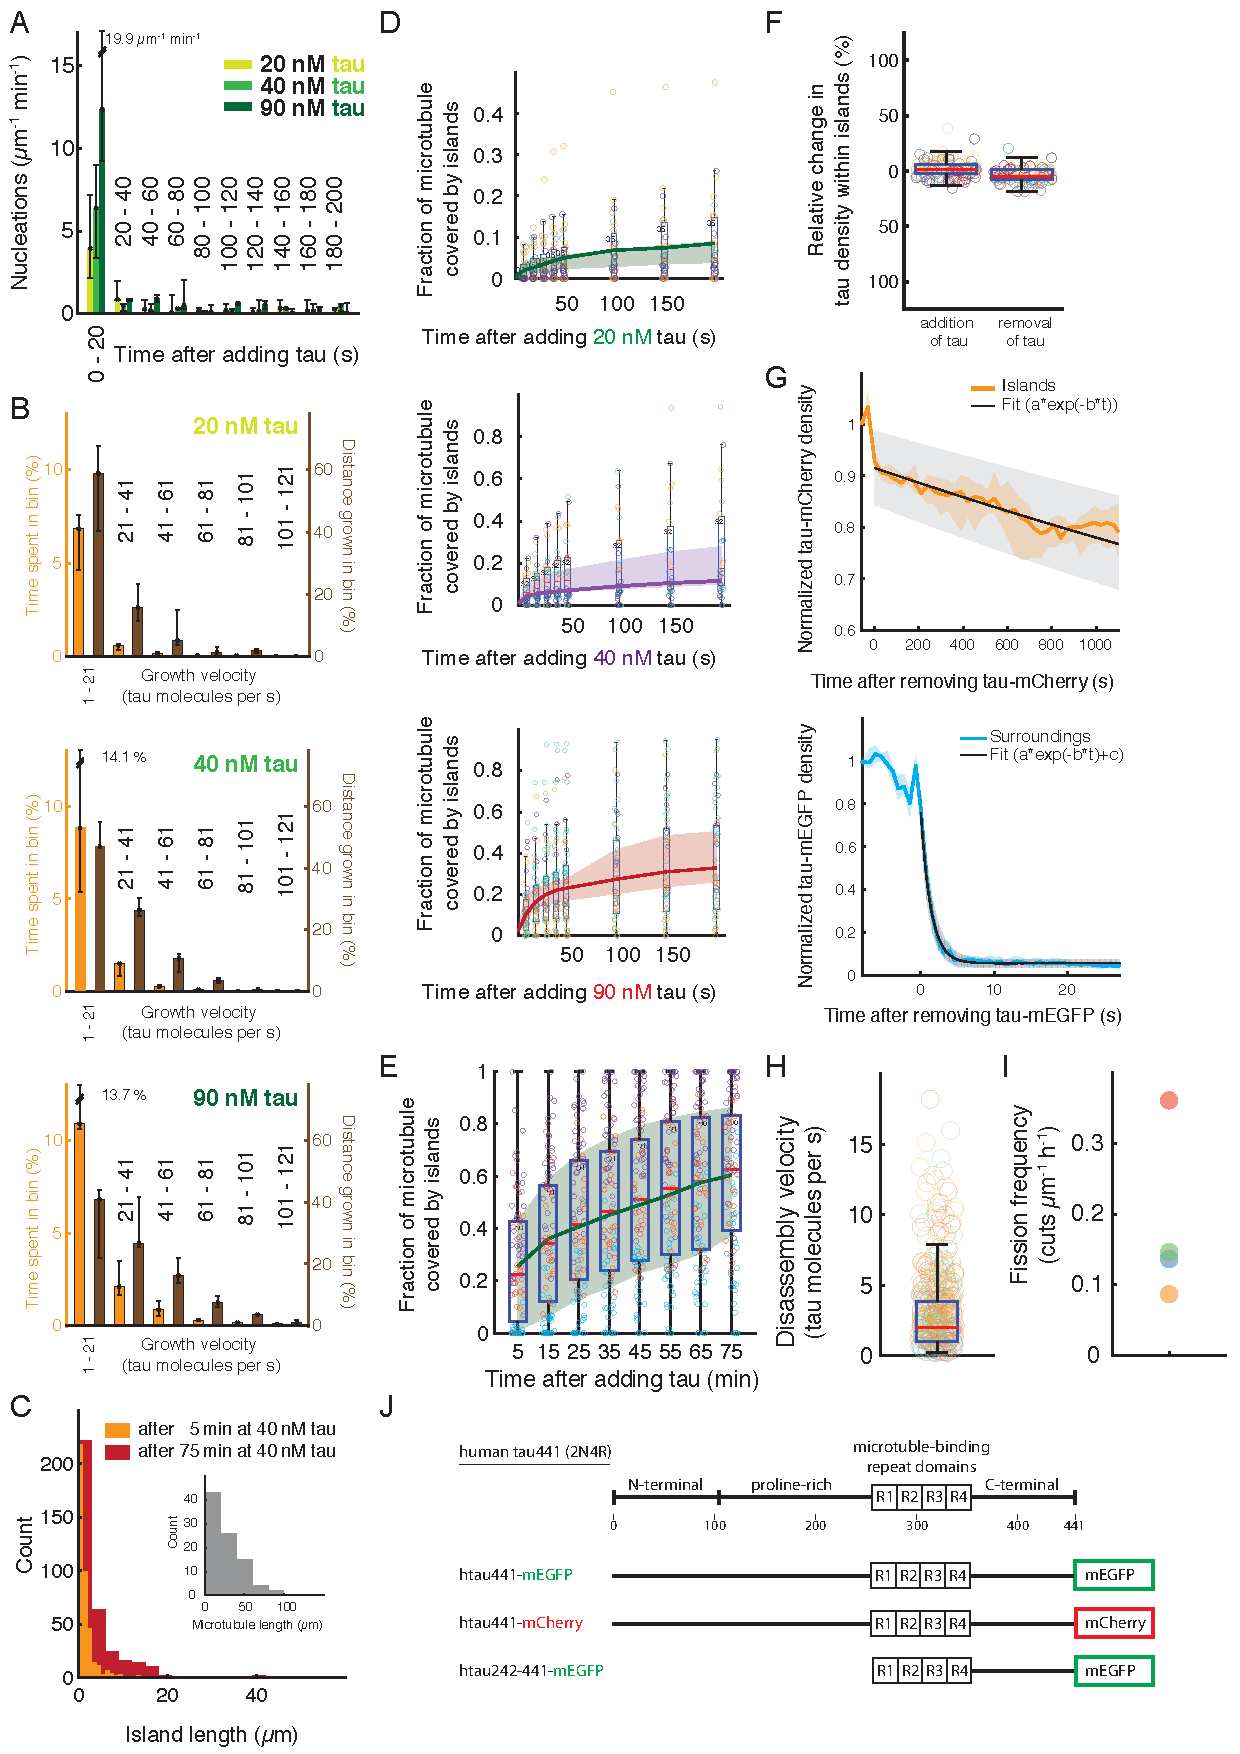
\includegraphics[scale=0.75]{Figures/tau_s1.pdf}
\caption[Supplementary figure for: Tau on microtubules separates into two kinetically distinct phases.]{
Caption on next page.
	}\label{tau_s1}
\end{figure}
\begin{figure}[t]
  \caption{
 (A) Distribution of time between the addition of tau-mEGFP and the formation of the islands (3 experiments per condition, n = 610 nucleation events). Bars show the median; error bars show the minimum and the maximum value. Same experiments as presented in (B) and (D). (B) Histograms of island growth velocities at different tau concentrations in solution (Methods, n = 2131 velocity traces). Same experiments and data representation as in (A). (C) Distribution of the lengths of islands 5 and 75 minutes after the addition of 40 nM tau-mEGFP, n = 91 microtubules in 3 experiments. Distribution of microtubule lengths is shown in the inset. Same experiments as presented in (E). (D) Fraction of microtubule length covered by tau islands at different concentrations of tau-mEGFP in solution. Solid lines and shaded areas (shown also in Figure 1E) represent the median and first and third quartiles values calculated over the whole fields of view (n = 3 experiments). Boxplots represent the same statistics calculated over individual microtubules (n = 40 microtubules for 20 nM tau, n = 32 microtubules for 40 nM tau and n = 59 microtubules for 100 nM tau). The same data as presented in Figure 1E, same experiments as presented in (A). (E) Island assembly does not cease even 75 minutes after the addition of 20 nM tau. The same data representation as in (D), same experiments as presented in (C). (F) Relative difference in tau density within islands i) just after the island nucleation upon the addition of tau and 30 seconds later and ii) just after the removal of tau and 30 seconds later (n = 91 microtubules in 16 experiments). Bleaching was not negligible in the case where tau was absent from solution – for a precise estimation of tau unbinding see (G). (G) Exemplary time-trace of tau-mCherry density inside and tau-mEGFP density outside the islands after removal of tau (mCherry- or mEGFP-labeled, respectively) from solution, analogous to the results presented in Figure 1H (n = 6 microtubules). Single exponential fits are indicated by solid lines. This experiment had been repeated 4 and 3 times for islands and surroundings, respectively, with similar results. Time constants derived from fits for all experiments are shown in Figures 2B and S2D. (H) Distribution of island disassembly velocities upon removal of tau from solution yielding the average velocity of 6.6 ± 5.2 nm/s (average ± SD, corresponding to 2.9 ± 2.3 tau molecules unbinding per second, Methods). Colors encode experiments (n = 335 velocity traces on 90 islands in 4 experiments). For a description of all boxplot elements see Methods. (I) Frequency of fissions occurring within islands upon removal of tau from solution yielding the average 0.20 ± 0.14 fissions per micron of island length per hour (average ± SD). Colors encode n = 4 experiments - same as in (H). (J) Schematics showing the tau constructs used in this study.
  }
\end{figure}
\begin{figure}[h!tb]
\centering
%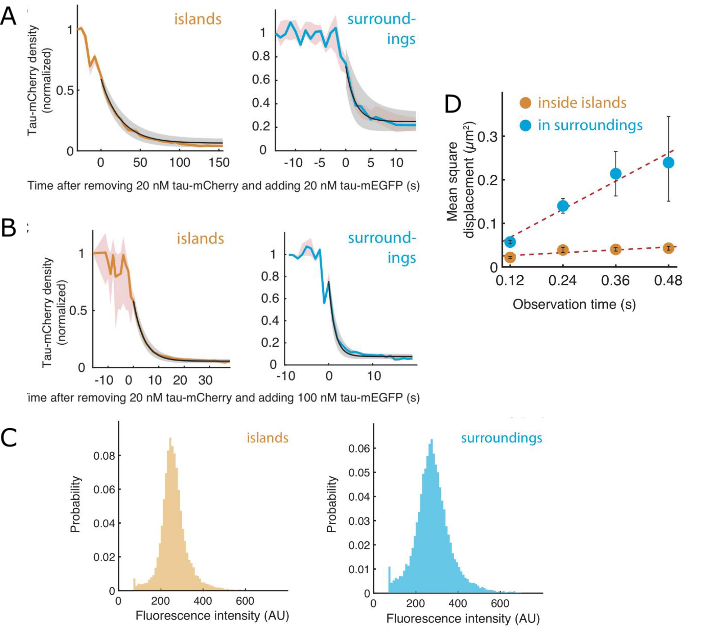
\includegraphics[scale=0.75]{Figures/tau_s2.png}
\caption[Supplementary figure for: Tau molecules in the islands are stationary but exchange with tau in solution.]{
(A) Exemplary time-trace and fit of tau-mCherry density inside and outside the islands after exchange of 20 nM tau-mCherry for 20 nM tau-mEGFP (n = 5 respectively 7 microtubules). Photo-bleaching during these experiments was negligible (Methods). This experiment had been repeated 5 and 2 times for islands and surroundings, respectively, with similar results. Time constants derived from fits for all experiments are shown in Figures \ref{tau2}C and D. (B) Analogous estimation of tau residence times as in (A) for an exemplary experiment in which 20 nM tau-mCherry was exchanged for 100 nM tau-mEGFP (n = 5 microtubules). The photo-bleaching during this experiment was negligible (Methods). This experiment had been repeated 4 and 2 times for islands and surroundings, respectively, with similar results. Time constants derived from fits for all experiments are shown in Figures \ref{tau2}C and D. (C) Histogram of fluorescence intensities of single tau-mEGFP particles bound to microtubules in experiments as presented in Figure \ref{tau2}E, showing that tau-mEGFP is associated with the microtubule in monomeric form (n = 1861 molecules inside the islands, n = 2210 molecules outside the islands, 1 experiment). (D) Mean square displacement over time of single tau-EGFP molecules inside and outside the islands yielding tau diffusion constants of 0.27 ± 0.15 µm2s-1 (95\% confidence bounds, n = 3660 molecules) outside the islands and 0.027  ± 0.016 µm2s-1 (95\% confidence bounds, n = 2558 molecules, 3 experiments) inside the islands. For comparison, the analogously estimated diffusion constant of non-motile kinesin-1 molecules tightly bound to the microtubule in the presence of AMP-PNP (in the absence of ATP) was 0.014 ± 0.016 µm2s-1 (95\% confidence bounds, n = 126 molecules, 1 experiment).
	}\label{tau_s2}
\end{figure}
\begin{figure}[h!tb]
\centering
%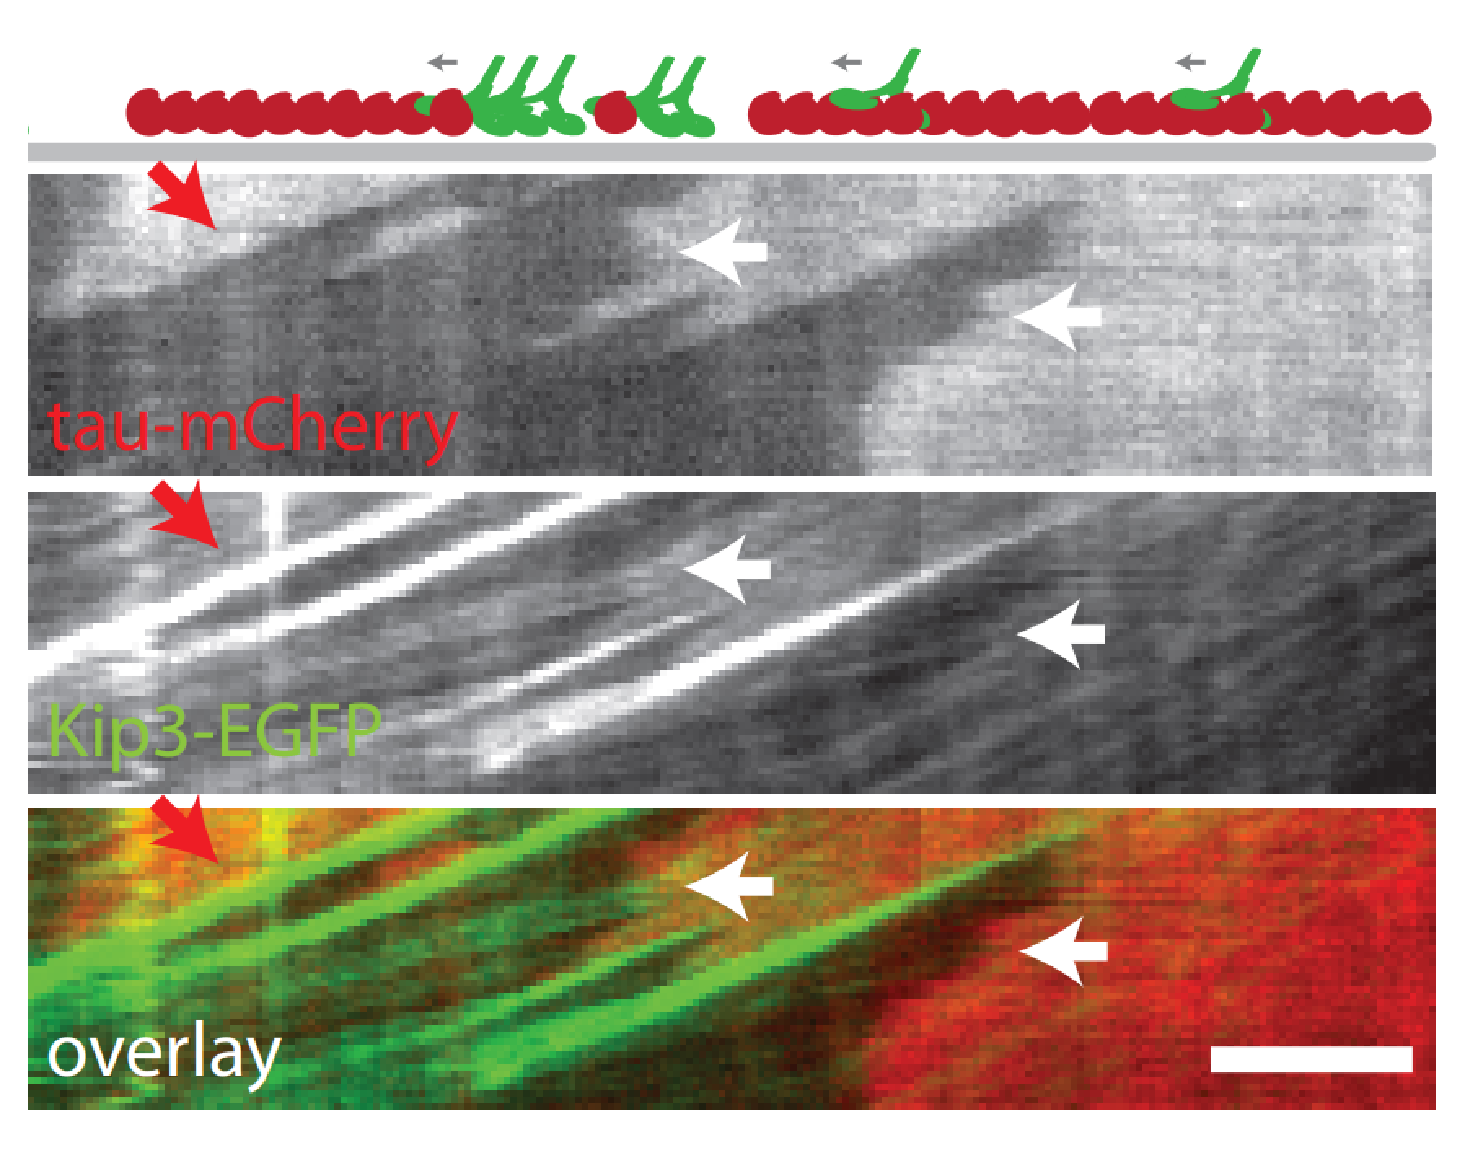
\includegraphics[scale=0.9]{Figures/tau_s4.png}
\caption[Supplementary figure for: Tau islands are distinguished by tau cohesion.]{ (A) Multichannel fluorescence kymograph showing the motion of kip3-GFP (green) inside and outside the tau islands (red). Red arrow indicates the accumulation of kip3-GFP in front of the island. White arrows indicate kip3-GFP molecules speeding up as they leave the island. Scale bar 2 µm. This experiment had been repeated 7 times with similar results. 
	}\label{tau_s4}
\end{figure}
\begin{figure}[h!tb]
\centering
%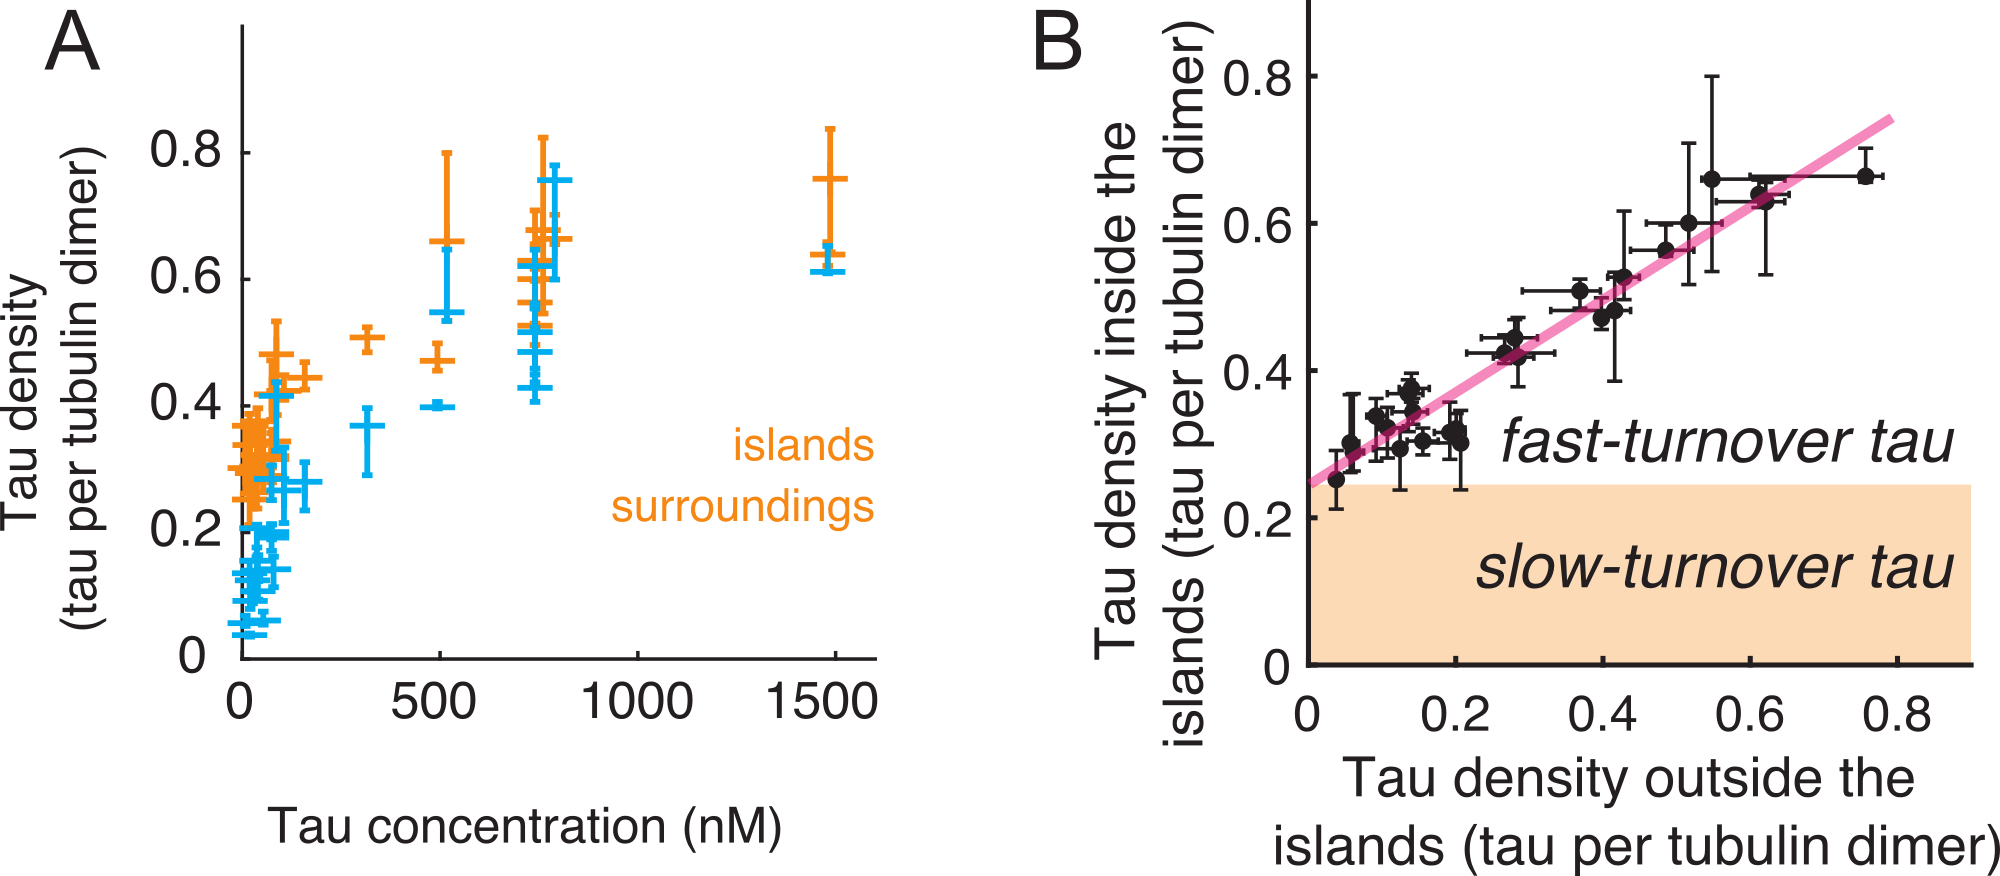
\includegraphics[scale=0.9]{Figures/tau_s5.png}
\caption[Supplementary figure for: Tau islands are distinguished by tau cohesion.]{
(A) The density of tau-mEGFP on the microtubules saturates at high (µM) tau-mEGFP concentrations (total of 29 and 27 experiments for islands and surroundings, respectively). Horizontal lines indicate the three quartiles. (B) At tau-mEGFP concentrations in the range of 20 nM to approximately 1 µM, the tau-mEGFP density inside the islands scales linearly with the tau-mEGFP density outside the islands. Points indicate medians, error bars indicate the first and third quartiles (both axes). Data from the experiments presented in (A).
	}\label{tau_s5}
\end{figure}

\begin{figure}[h!tb]
\centering
%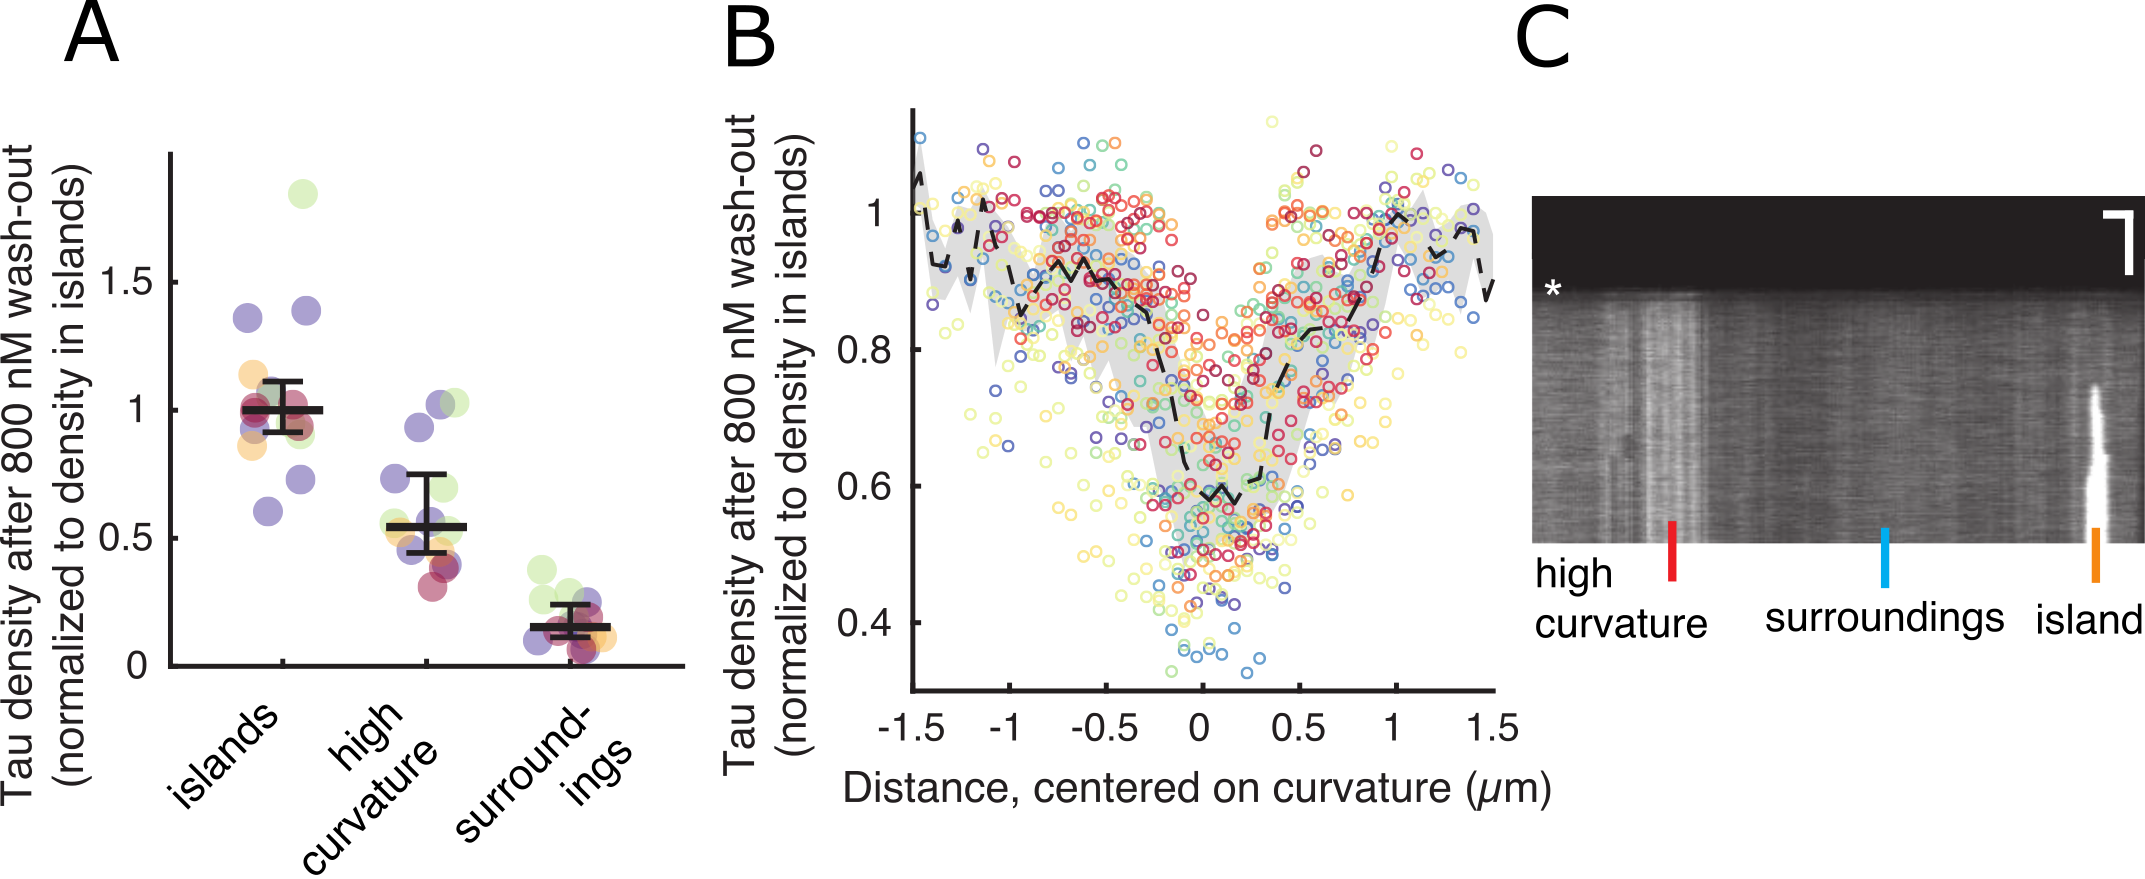
\includegraphics[scale=0.82]{Figures/tau_s7.png}
\caption[Tau islands do not form at regions of high microtubule curvature.]{
\textbf{Supplementary figure for: Tau islands do not form at regions of high microtubule curvature.} 
(A) Densities of tau-mCherry outside the islands, inside the islands and in the regions of high curvature (after the removal of 0.8 µM tau from solution). Points are color-coded by experiments, horizontal lines indicate the three quartiles, weighted such that each experiment has equal weight. 
(B) Tau density profile along the microtubule after removing 800 nM tau from solution. X-axis is centered on the point of highest curvature. Data are color-coded by microtubule and the density is normalized to the 90th percentile of the density-values of the respective microtubule. The red line represents the median of n = 30 microtubules (7 experiments), the first and third quartile are indicated by the shaded area. At 800 nM tau, there always were islands adjacent to microtubule bends, which is why the tau density to the left and right of the curved microtubule region is high even though tau has been removed from solution. A clear decrease in the tau density is apparent at the point of highest curvature.
(C) Kymograph showing the uniform increase of tau-mEGFP density along the whole region of the microtubule curve upon the addition of tau-mEGFP in solution. This is in strong contrast to islands localized on straight microtubules, which grew at their boundaries. Scale bars, vertical 10 min, horizontal 2 µm.
	}\label{tau_s7}
\end{figure}




\end{document}  